\documentclass[12pt,a4paper]{book}


\input{Files/Packages}

\input{Files/Macros}


\title{High Level Synthesis}
\author{Ranim Tom}


%******** Abbreviations **********

% to change the name of Nomenclature to list of abbreviation
\renewcommand{\nomname}{List of Abbreviations}

% for list of abbreviations and acronyms
\makenomenclature



\begin{document}


\maketitle

\tableofcontents

\listoffigures

\listoftables


% to make the list of abbreviations and acronyms appear 
% in first pages of the report
\printnomenclature


% to make the todo list appear as a table of content
\listoftodos

% To adjust the header in the report/book

\pagestyle{fancy}
\fancyhf{} % Clear header and footer
\rhead{\rightmark}
\lhead{Chapter \thechapter}
\rfoot{Page \thepage}

\part{Fundamental of HLS and Combinational Circuit}
\label{part:fundamentals}

\input{content/intro_hls}



\chapter{Input Output}



\section{LED program}

Our $\mathrm{1}^\mathrm{st}$ program to HLS will be driving some LED on.

Now we will proceede in each section for a specific step from programming until bitstream file used in the fpga.\\

\todo{LED Controller} \uti{LED Controller:}

\begin{itemize}

\item \textit{To re-write the statment properly with some images}

\item \textit{To illustrate again the concept of:}

	\begin{itemize}
	\item \textit{interfaces}
	
	\item \textit{Port and pins conncetion}
	
	\item \textit{Role of pragma directive}
	\end{itemize}

\end{itemize}


\subsection{Resource for the Vitis IDE}

Refer to \url{https://docs.amd.com/r/en-US/ug1399-vitis-hls/Building-and-Running-an-HLS-Component} to see:

\begin{itemize}

\item Vitis IDE structure

\item Different Steps when building and desiging an HLS component

\end{itemize}

\todo{Vitis IDE} \uti{Vitis IDE:}

\begin{itemize}

\item \textit{To illustrate and make some introduction about the content of the url}

\item \textit{Mainly about:}

	\begin{itemize}
	
	\item \textit{The steps and the process}	
	
	\item \textit{The options in Vitis IDE with some images}
		
	\end{itemize}


\end{itemize}


\subsection{Generating IP Package}

After running successfully the \verb|C| simulation step, we need to generate an IP pacakge. This package can be used in \verb|Vivado| software so we can generate the bitstream file which will be used to program the FPGA.\\

\underline{Generating the IP Pacakge:} under the flow navigator, run the \verb|Package| command, and we should specify the 


\subsection{Vivado}

Now we are ready to generate the bitstream file. For that, open \verb|Vivado|, and create a project.\\

Then \verb|Create IP block diagram|.

Under \verb|Settings|, search for the \verb|IP| workspace, and \verb|Vivado| will search for any \verb|IP| in the selected workspace.



We can search for our \verb|IP| name (\verb|basic_output|), then using the search bar select the \verb|IP| name we want, and the block will be imported to \verb|Vivado| as shown in \autoref{fig:input_output:ip_block}.

\begin{figure}[h]
\centering
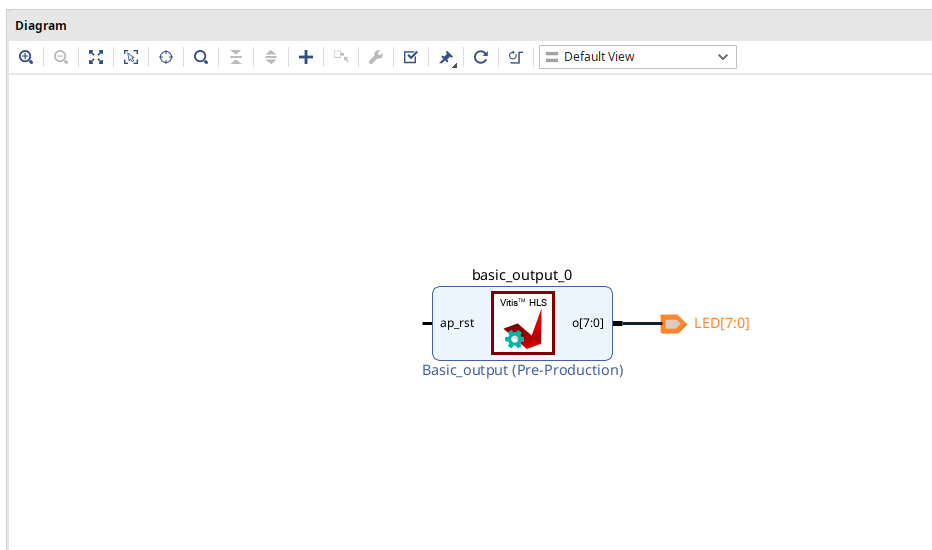
\includegraphics[scale=0.5,frame]{Figures/input_output/ip_block}
\caption{IP Block for LED controller}
\label{fig:input_output:ip_block}
\end{figure}


\underline{Port to FPGA Pins: Constrains}\\

Now to make connections form the port of the \verb|IP| to the FPGA pins, we need to some constraints. To add these constraints, go \verb|Sources|, right click on \verb|Constraints| folder and select \verb|Add Sources|.\\

After that we select \verb|Create Constraint| option, and then choose a file name.\\

We copy paste the constraint file forom \verb|digilent| gihtub for basys3 board (\url{https://github.com/Digilent/Basys3/tree/master}). under \verb|Resources| folder.\\

Finally we uncomment the $\mathrm{1}^\mathrm{st}$ 8 LED in the LED sections.












\chapter{Combinational Circuit}


\section{Review of Combinational Circuit}

In this section, we review fundamental concepts on digital circuit and logic desing, and mainly the one encountered in \verb|HLS|. \\


\subsection{Combinational Circuit}

$\mathrm{1}^\mathrm{st}$, recall that a combinational circuit are circuit in which \tbi{outputs depends only in current states of the input}, therefore any change in input affect the output after some delay.

Also, a combinational circuit doesn't have or use any memory or storage device. \autoref{fig:combinational_circuit:app_comb_circuit} presents applications of combinational circuit.


\subsection{Logic Gates}

\todo{Logic Gates} \uti{Logic Gates}

\begin{itemize}

\item \textit{Source: Section 6 video 39}

\item \textit{Contains some nice picture, maybe to insert them later in my summary report}

\end{itemize}


\newpage
\begin{figure}[h]
\centering
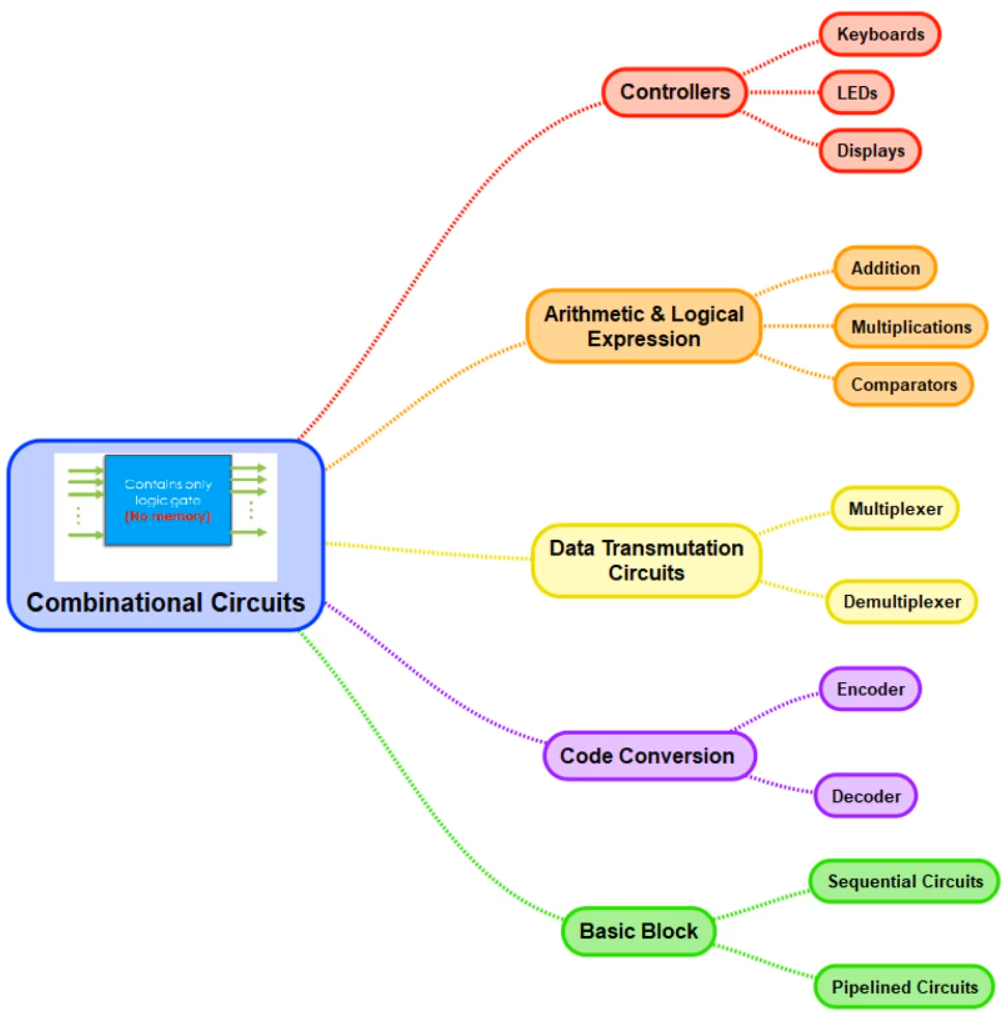
\includegraphics[scale=0.45,frame]{Figures/combinational_circuit/app_comb_circuit}
\caption{Combinatial Circuit Applications}
\label{fig:combinational_circuit:app_comb_circuit}
\end{figure}

\newpage
\section{Propagation Delay}
\label{sec:prop_delay}

Logic gates doesn't react to input instantly, it takes some time in order correct output is computed. In \autoref{fig:combinational_circuit:delay_gate_example}, an example of NAND gate delay is shown.


\begin{figure}[h]
\centering
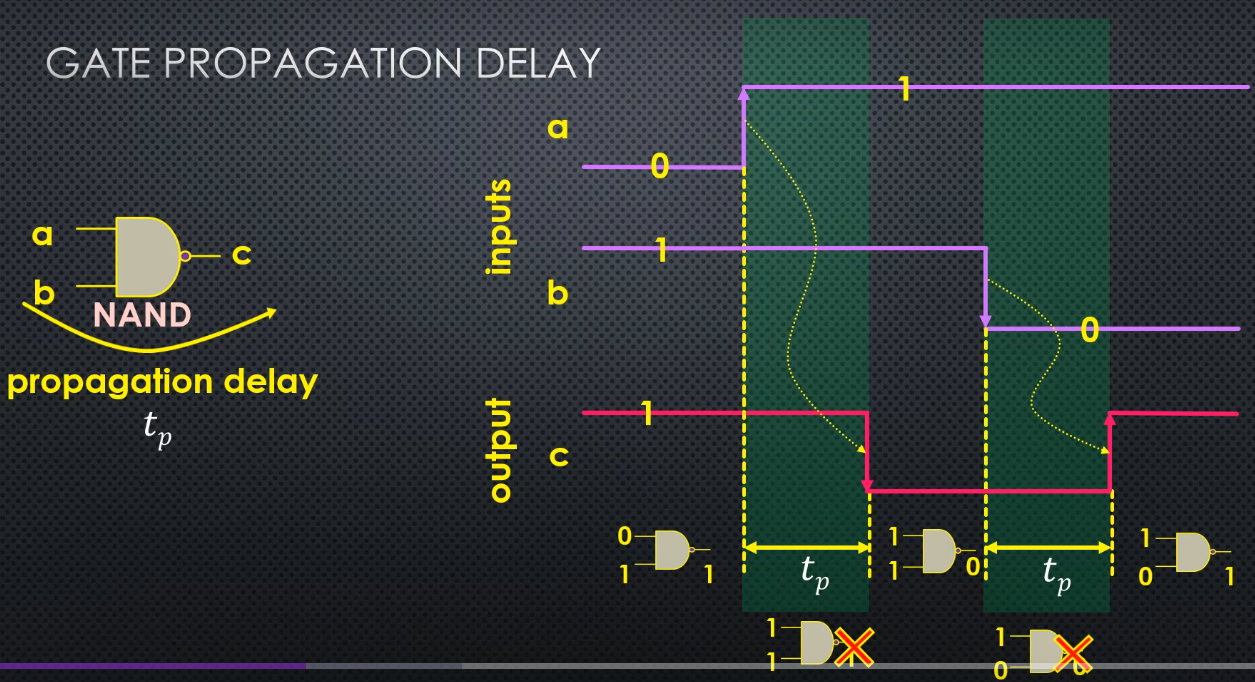
\includegraphics[scale=0.40,frame]{Figures/combinational_circuit/delay_gate_example}
\caption{Propagation Delay Example using NAND gate}
\label{fig:combinational_circuit:delay_gate_example}
\end{figure}

\begin{itemize}

\item When state of $a$ changes from 0 $\rightarrow$ 1, the output didn't appear instantly, it appears after some delay $t_p$

	\begin{itemize}
	\item During this period $t_p$, the output of the NAND gate in invalid and it shouldn't take into accounts
	\end{itemize}

\item Same thing when state of $b$ changes from 1 $\rightarrow$ 0

\end{itemize}

\newpage
The concept of delay also apply to combinational circuit, as it shown in \autoref{fig:combinational_circuit:delay_comb_circuit_example}.

\begin{figure}[h]
\centering
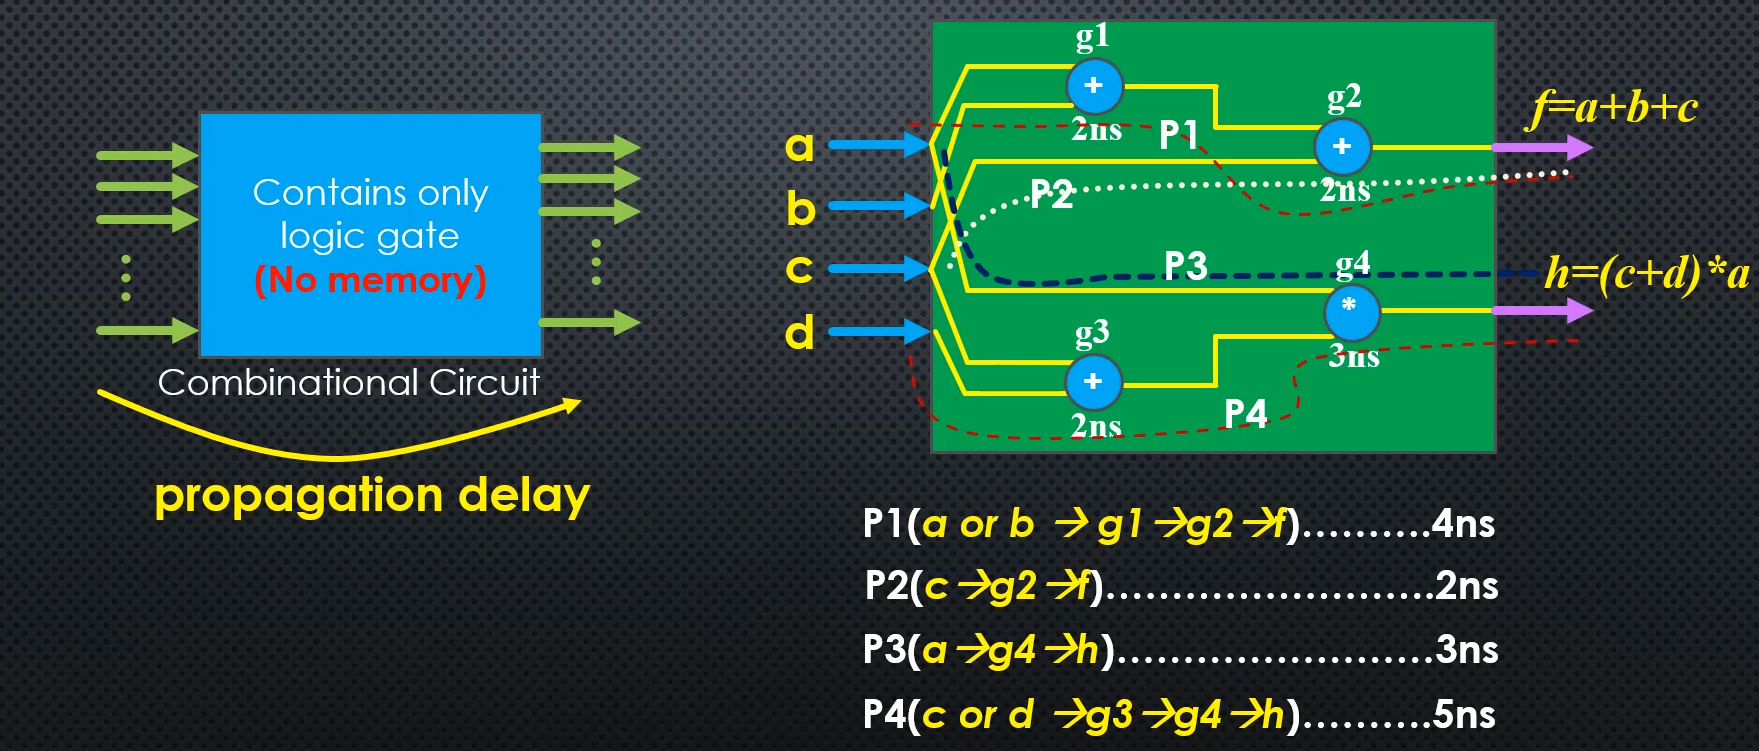
\includegraphics[scale=0.27,frame]{Figures/combinational_circuit/delay_comb_circuit_example}
\caption{Propagation Delay Example in a combinational circuit}
\label{fig:combinational_circuit:delay_comb_circuit_example}
\end{figure}

\begin{itemize}

\item A combinaotional circuit consists of many path, and each path has a certain delay

\item The path with maximum delay is called the \tbi{critical path}

\item we have 4 path $P_i$ and 4 operators $g_i$

\item $P_4$ is the critical path since it has the longest propagation delay

\end{itemize}


In \verb|HLS| desing, \tbi{the goal is to minimize this propagation delay as possible}

\subsection{N Bit Binary Adder}

Let't take an example of computing delay for full binary adder. Its circuit is shown in \autoref{fig:combinational_circuit:full_adder}.

\begin{figure}[h]
\centering
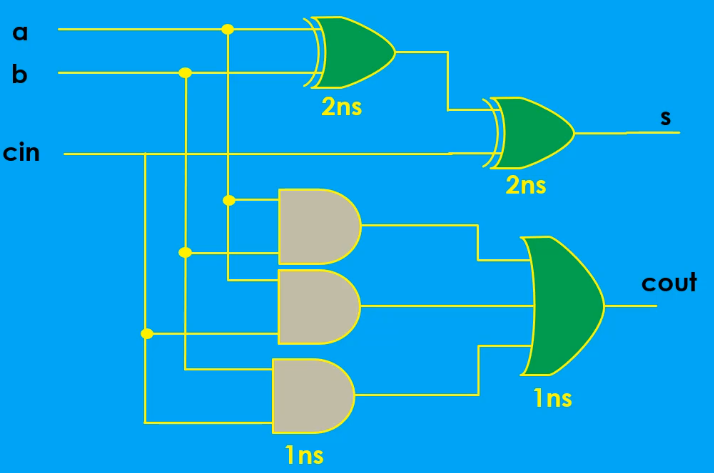
\includegraphics[scale=0.30,frame]{Figures/combinational_circuit/full_adder}
\caption{Full adder circuit}
\label{fig:combinational_circuit:full_adder}
\end{figure}

\newpage
All the path with there delays are shown in \autoref{fig:combinational_circuit:full_adder}.

\begin{figure}[h]
\centering
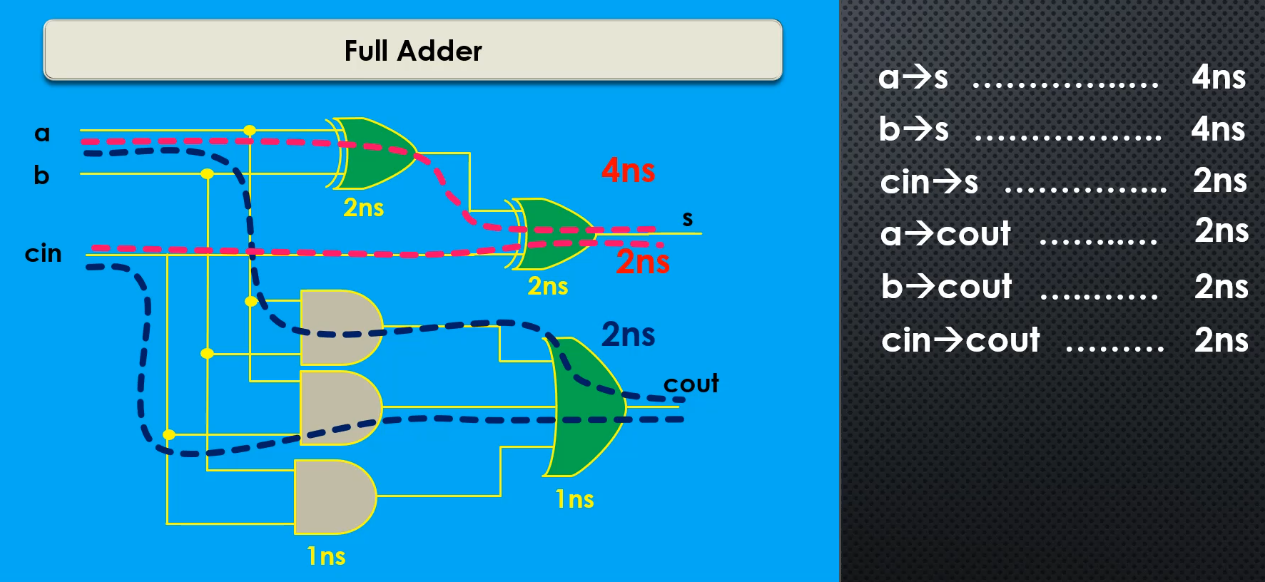
\includegraphics[scale=0.30,frame]{Figures/combinational_circuit/full_adder_delay}
\caption{Delay path for full adder}
\label{fig:combinational_circuit:full_adder_delay}
\end{figure}

So it appears that a full adder output can be used of 4 ns, and any change of the input is not valid till this 4 ns eplases.\\

Now a $N$ bit binary adder can be designed using the \textit{ripple design} shown in \autoref{fig:combinational_circuit:ripple_desing_adder}, where the output carry bit $C_{\text{out}_n}$ is connected to the next adder carry input $C_{\text{in}_{n+1}}$


\begin{figure}[h]
\centering
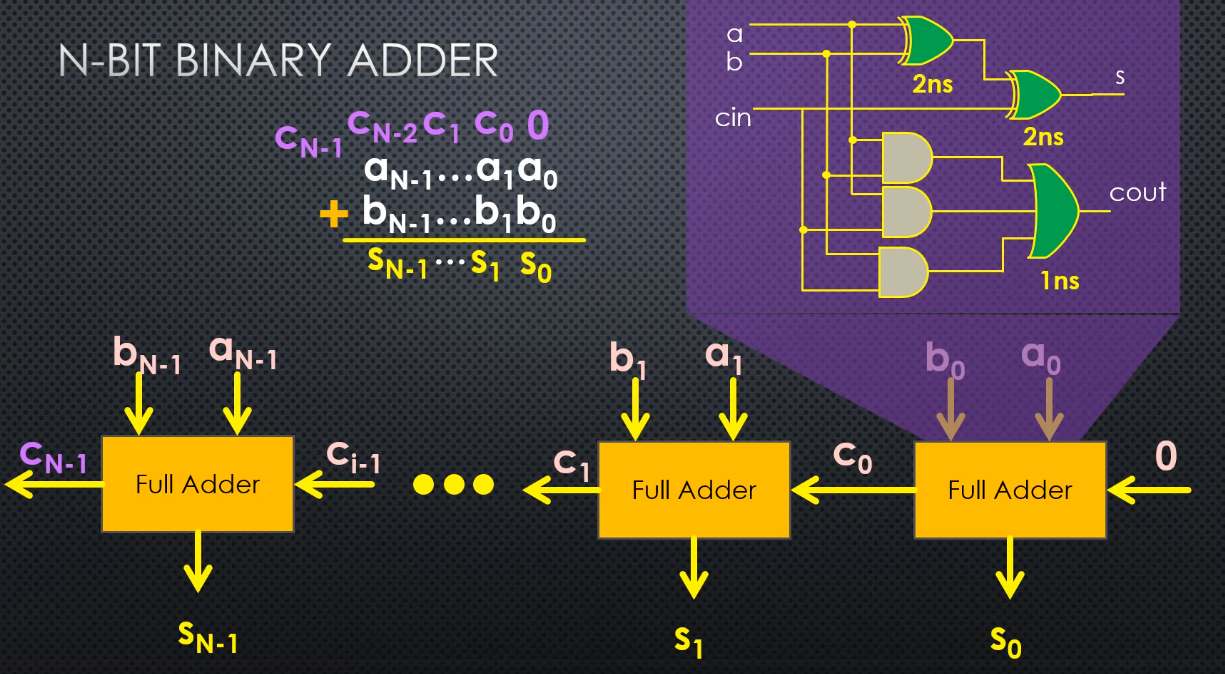
\includegraphics[scale=0.30,frame]{Figures/combinational_circuit/ripple_desing_adder}
\caption{N bit binary adder}
\label{fig:combinational_circuit:ripple_desing_adder}
\end{figure}

\newpage
Each full adder circuit in the $N$ bi adder has 3 path delay shown in  \autoref{fig:combinational_circuit:N_adder_path}

\begin{figure}[h]
\centering
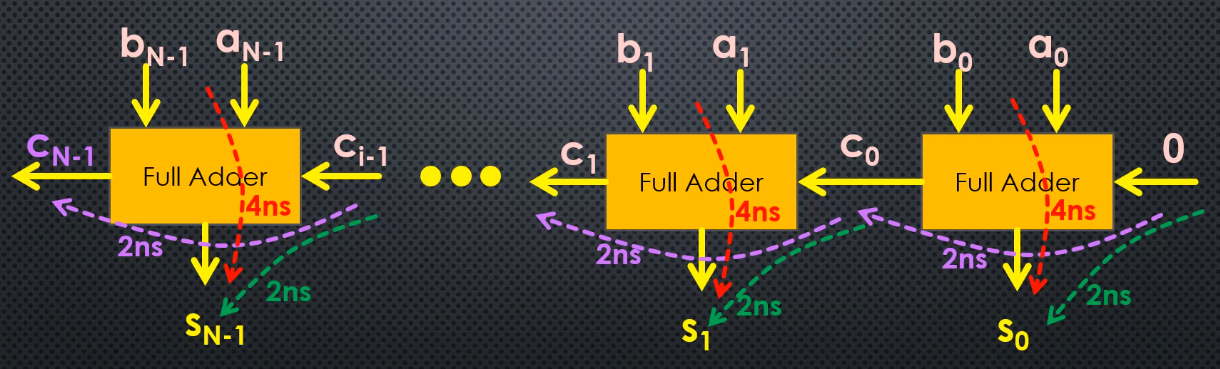
\includegraphics[scale=0.30,frame]{Figures/combinational_circuit/N_adder_path}
\caption{N bit binary adder delay path}
\label{fig:combinational_circuit:N_adder_path}
\end{figure}

\begin{itemize}

\item from $a_n$ and $b_n$ input to $s_n$ output

\item from carry input to sum: $c_{\text{in}_n} \, \longrightarrow \,  s_n$

\item from carry input to carry output: $c_{\text{in}_n} \,  \longrightarrow \,  c_{\text{out}_n}$


\end{itemize}

Now if we want to trace the delay of the $N$ bit adder circuit, we are interested in carry bit and sum bit. Referring back to \autoref{fig:combinational_circuit:full_adder}, the delay from carry input bit to sum bit is 2 ns. The tracing for $N$ bit binary adder is shown in \autoref{fig:combinational_circuit:N_adder_trace_delay}.

\begin{figure}[h]
\centering
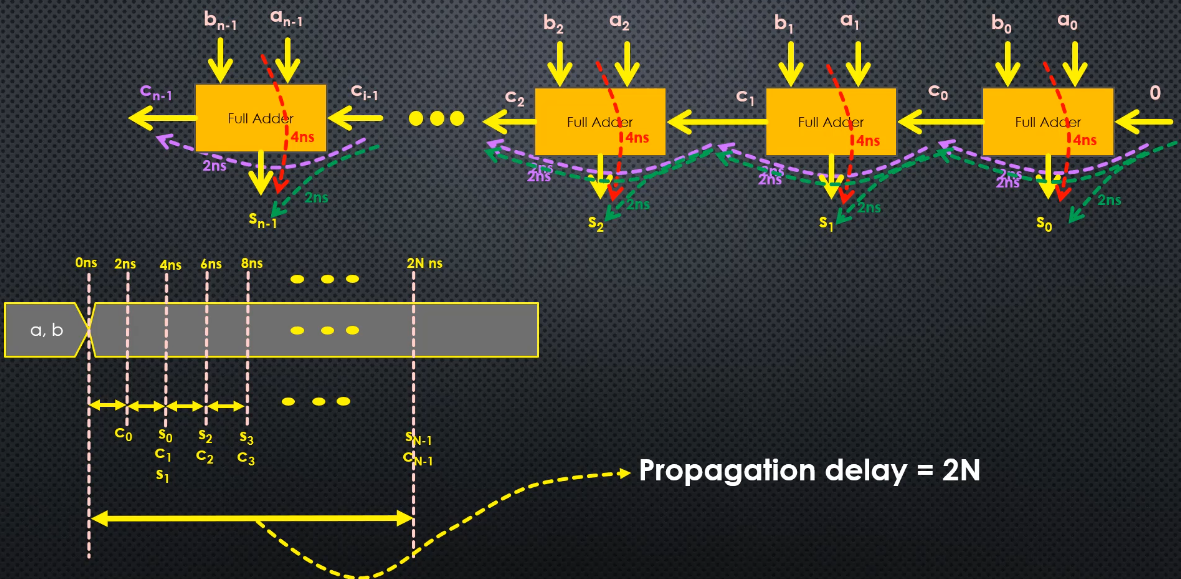
\includegraphics[scale=0.30,frame]{Figures/combinational_circuit/N_adder_trace_delay}
\caption{N bit binary adder: tracing delay}
\label{fig:combinational_circuit:N_adder_trace_delay}
\end{figure}

\begin{itemize}

\item We are assuming that input $a_n$ and  $b_n$ are available at 0 ns

\item Each $n-1$ adder needs 2 ns cycle for the sum and carry bit to be ready

\item We have $N$ adder so the total delay is equal to $2\, N$ ns
\end{itemize}

\newpage
\section{Combinational Circruit in HLS}

Now suppose we have some combinational circuit with some function to represent it, how can we immplement or represent it in \verb|HLS|?

An example is shown in \autoref{fig:combinational_circuit:example_comb_circuit}, where we can represent the function $d$ using 2 types of operators:

\begin{itemize}

\item Bitwise Operator

\item Logical Operator

\end{itemize} 

\begin{figure}[h]
\centering
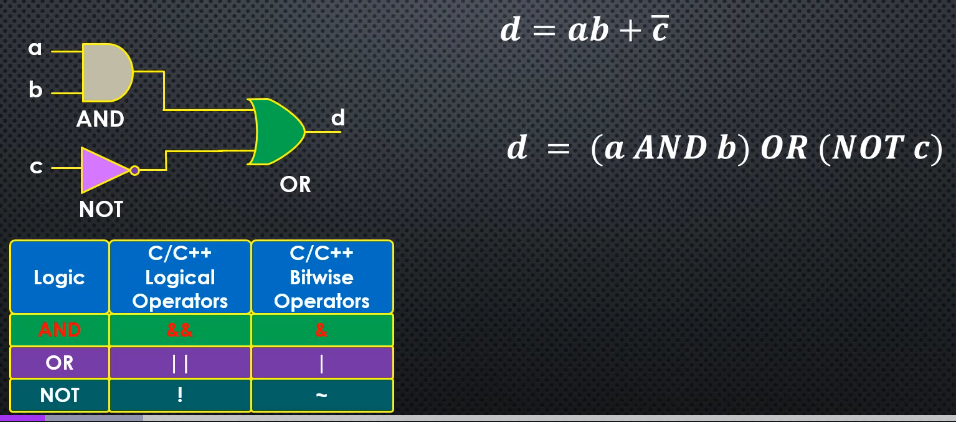
\includegraphics[scale=0.35,frame]{Figures/combinational_circuit/example_comb_circuit}
\caption{Example of a combinational circuit}
\label{fig:combinational_circuit:example_comb_circuit}
\end{figure}

The equivalent \verb|HLS| code is shown in \autoref{fig:combinational_circuit:HLS_comb_circuit}

\begin{figure}[h]
\centering
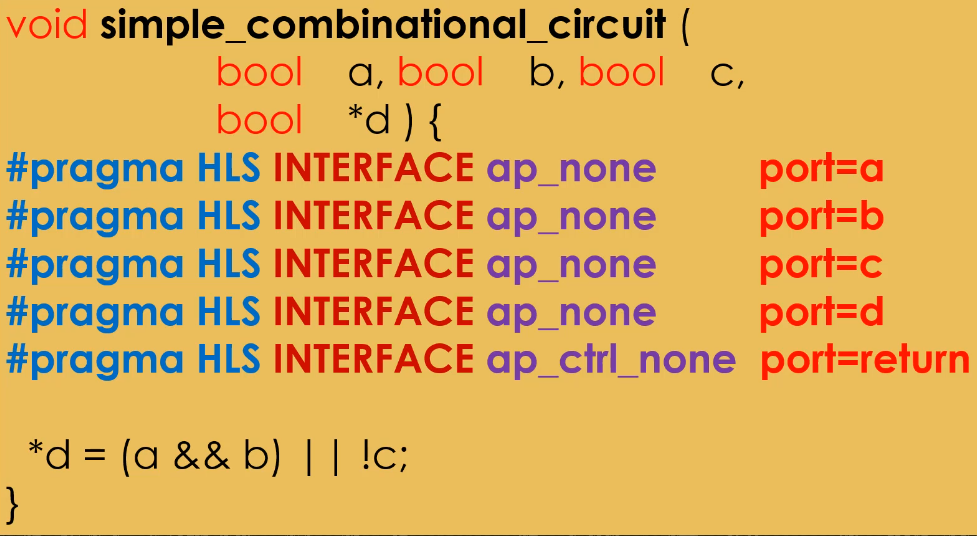
\includegraphics[scale=0.30,frame]{Figures/combinational_circuit/HLS_comb_circuit}
\caption{HLS code for \autoref{fig:combinational_circuit:example_comb_circuit}}
\label{fig:combinational_circuit:HLS_comb_circuit}
\end{figure}

\begin{itemize}

\item Since we are using wires to represent input and output, \verb|ap_none| interface is used for the function arguments

\end{itemize}

\newpage
\subsection{Synthesis Report}

After the function is synthesised using \verb|Vitis|, the report gives us 3 important part, shown in \autoref{fig:combinational_circuit:comb_circuit_report}.


\begin{figure}[h]
\centering
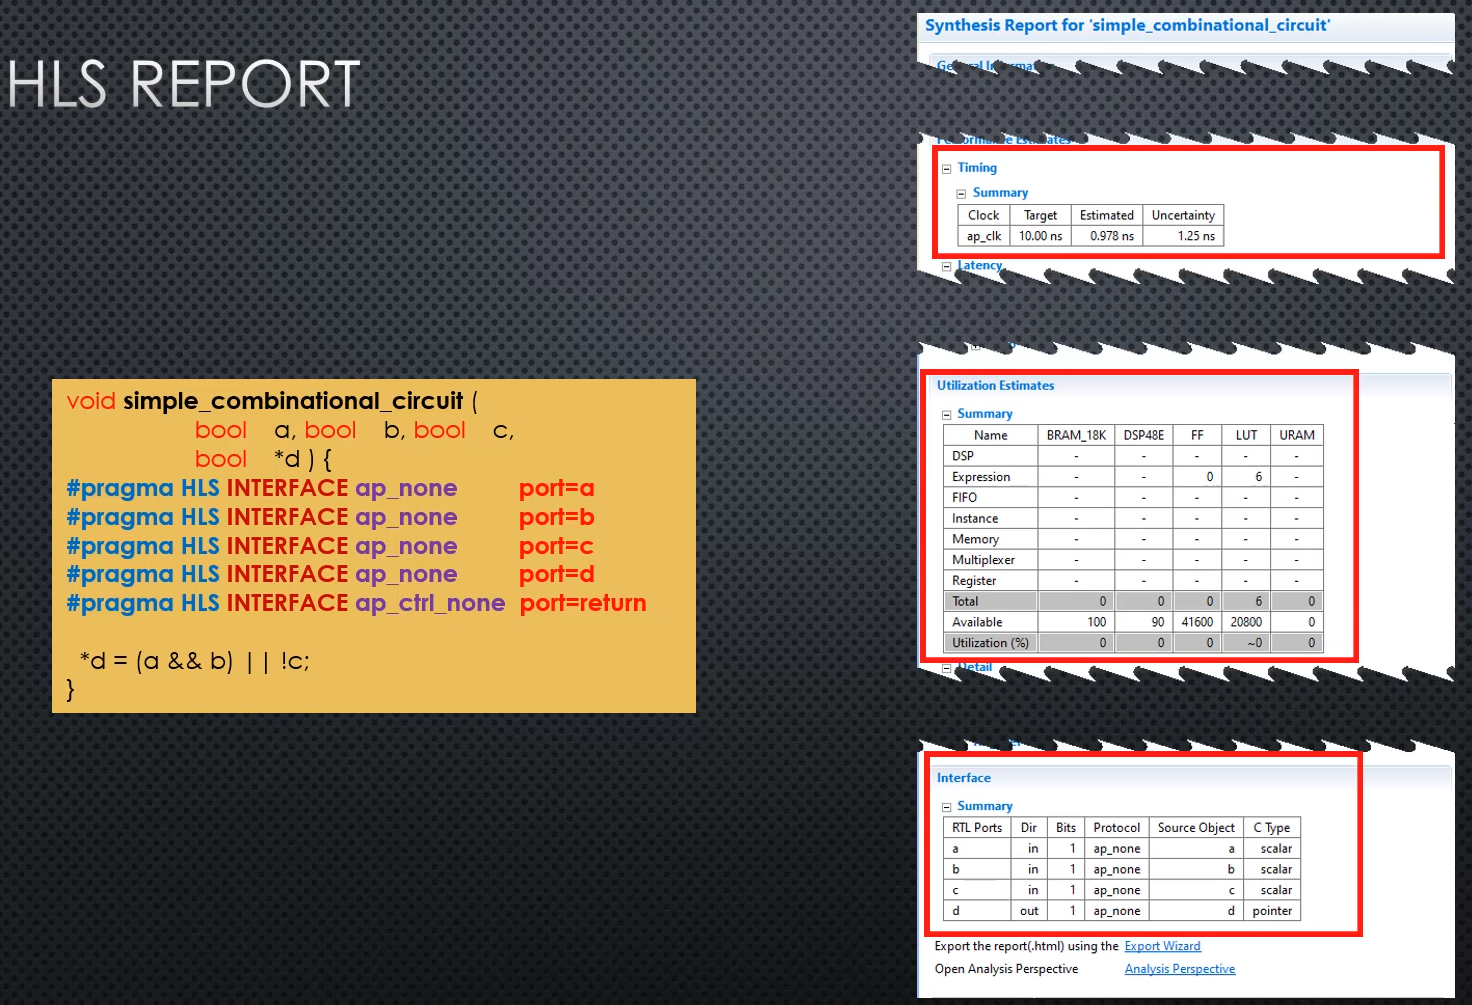
\includegraphics[scale=0.35,frame]{Figures/combinational_circuit/comb_circuit_report}
\caption{Report generation}
\label{fig:combinational_circuit:comb_circuit_report}
\end{figure}

\begin{itemize}

\item Timing part: more for sequential circuit, we skip it for now

	\begin{itemize}
	\item However, we are interested in \textit{estimated} column, where it give us an estimation of $t_p$
	\end{itemize}

\item Resource Utilization: there are the resources we use to synthesize the circuit.

	\begin{itemize}
	\item 3 of the 5 columns are for memory (BRAM,FF,URAM). They should be 0 when dealing with combinational circuit
	
	\item The other 2 are LUT, for logical expression and DSP for mathematical operation, especically for floating point
	\end{itemize}

\item Interface: if for the function arguments part

\end{itemize}


\newpage
\section{Summary}

\begin{itemize}

\item \verb|HLS| desing goal: minimize $t_p$ (\ref{sec:prop_delay})

\item Output of combinational circuit is not valid till $t_p$ elapses

	\begin{itemize}
	\item Also any change of input values, is not valid also till $t_p$ elpases
	\end{itemize}


\end{itemize}






\chapter{Testbench and Simulation}

\section{Introduction}

After writing some code and implementing some project in \verb|HLS|, it is time to explore the concept of \textit{testbench} and \textit{simulation}.\\

Testbench and simulation are techniques in order to validate our \verb|HLS| desing. We can validate 2 things using these concpets:

\begin{itemize}

\item functional features such as the outputs: make sure we have the correct output for some given input

\item Non-functional featrures such as timing, power consumption,$\cdots$

\end{itemize}


\autoref{fig:testbench:testbench_concept} contains the concept of a testbench

\begin{figure}[h]
\centering
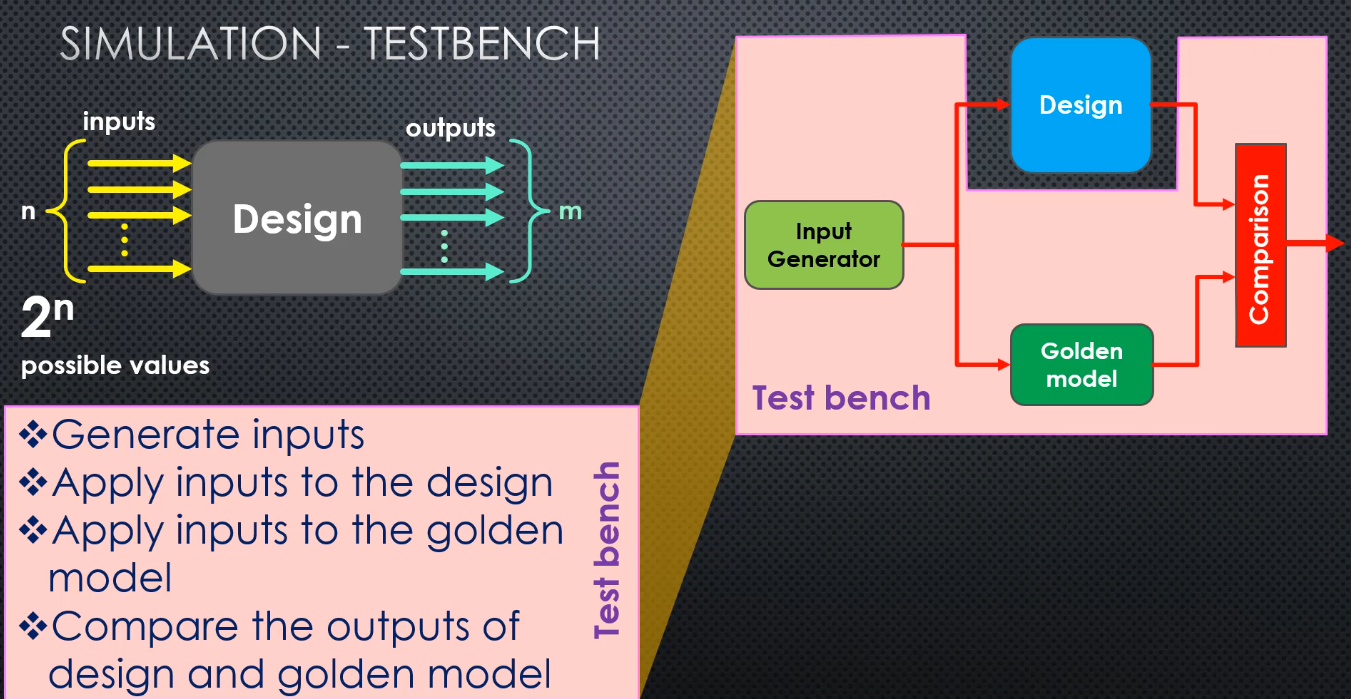
\includegraphics[scale=0.35,frame]{Figures/testbench/testbench_concept}
\caption{Testbench Concept}
\label{fig:testbench:testbench_concept}
\end{figure}

\begin{itemize}

\item Testbench is a \textit{software verification technique}, that is it relies entirely on a software approach to verify the desing

	\begin{itemize}
	\item Some other approach called \textit{emulation} rely on a software and hardware approach, in which we verify the result on the hardware target
	\end{itemize}

\item The job of a tesbench is to compare the results between our model and some state of art model using the same set of inputs, and compare the resutls to see if any differences exist

\end{itemize}

\newpage
\section{Testbench in Vitis}

Now we explore the concep using the \verb|Vitis| tool. In \verb|Vitis|, tesbench are know under the concept of \textit{C-simulation}. To understand the concept in \verb|Vitis|, we first start by recalling the classical known approach done in chapters before, that is without testbench. This approach is shown in \autoref{fig:testbench:hls_normal_flow}

\begin{figure}[h]
\centering
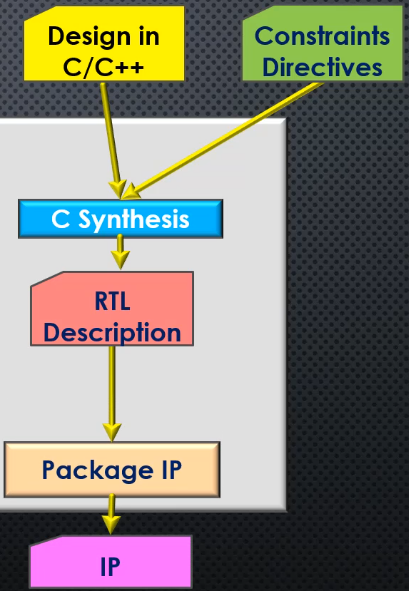
\includegraphics[scale=0.40,frame]{Figures/testbench/hls_normal_flow}
\caption{HLS Normal desing flow}
\label{fig:testbench:hls_normal_flow}
\end{figure}

\begin{itemize}

\item Using constraint file (\verb|.xdc|) and some \verb|C| code file, we generate the \verb|RTL| code (\verb|VHDL| and \verb|Verilog|) using \verb|C Synthesis| step in \verb|Vitis|.

Then in the $\mathrm{2}^\mathrm{nd}$ step, we generate the \verb|IP| so we can use it in \verb|Vivado| and generate the bitstream file to program the FPGA board.

\end{itemize}

Now to start the \textit{simulation flow}, we need 2 things: 

\begin{itemize}

\item testbench file

\item the \verb|C| files which contains the desing

\end{itemize}

\newpage
In simulation, constraint files are not needed. Using only the testbench and design \verb|C| files, we can perform \verb|C Simulation|, to correct all functional errors if any exist, and then \verb|C Sysnthesis| can be redone again to generate the \verb|RTL| code, as shown in \autoref{fig:testbench:hls_simulation}

\begin{figure}[h]
\centering
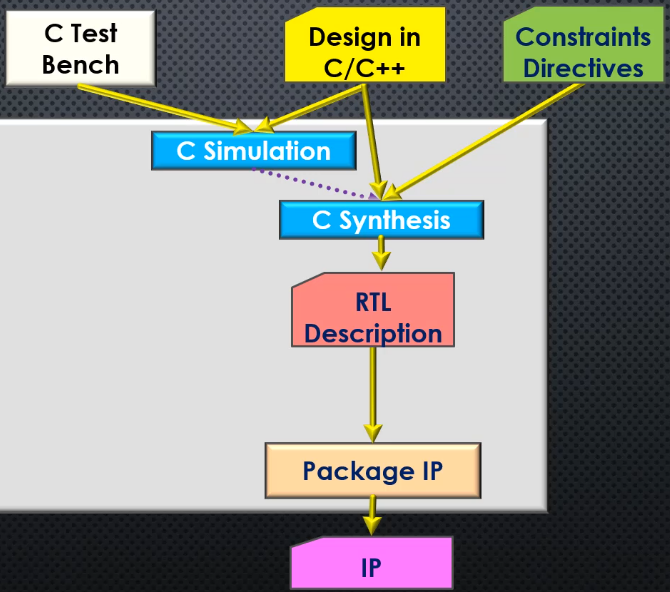
\includegraphics[scale=0.40,frame]{Figures/testbench/hls_simulation}
\caption{HLS Simulation using testbench and desing files}
\label{fig:testbench:hls_simulation}
\end{figure}


The \textit{regenerate RTL code} can also be verified, by a process called \tbi{C- RTL cosimulation}. In this process, \verb|HLS| \textit{re-uses} the testbench, and apply it on the re-gerenrate \verb|RTL|. We can check timing as well as the functinanlity in cycle accurate debug environment. 

After checking the regerenated \verb|RTL| files, the hardware \verb|IP| can be regenerate again. These steps are shown in \autoref{fig:testbench:rtl_rechecking}.


\begin{figure}[h]
\centering
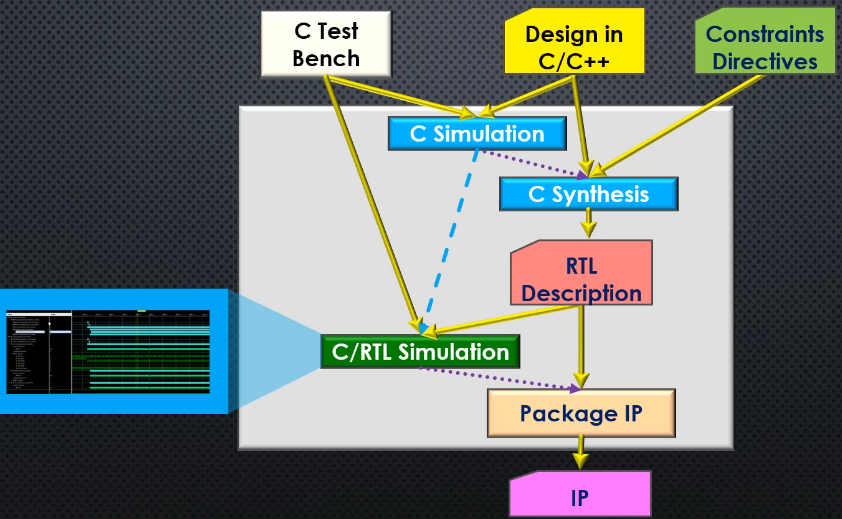
\includegraphics[scale=0.40,frame]{Figures/testbench/rtl_rechecking}
\caption{Rechecking the re-gerenated RTL code}
\label{fig:testbench:rtl_rechecking}
\end{figure}






\chapter{Data Types}
\label{chap:data_types}

\section{Introduction}

Choosing the right data types plays an important role in writing an otpmized code and deploy it to target. This chapter explains the data type options in \verb|HLS| and their related optimisation and development techniques.

\todo{data types intro} \uti{data types intro:}

\begin{itemize}

\item \textit{To adjust the introduction later}

\item \textit{This chapter needs I think a review about data types in C and C++}

	\begin{itemize}
	\item \textit{To see if there exist some differences between the 2 languages}
	
	\item \textit{To make link if possible between data types in a PC, MCU and FPGA}
	\end{itemize}

\end{itemize}

\newpage
\section{Native Data Types}

Programming languages such as \verb|C| and \verb|C++| support some native or builtin data types (\verb|char|,\verb|int|,$\cdots$), which can be modified using \textit{modifiers}, such as \verb|signed|,\verb|short|,$\cdots$

\begin{figure}[h]
\centering
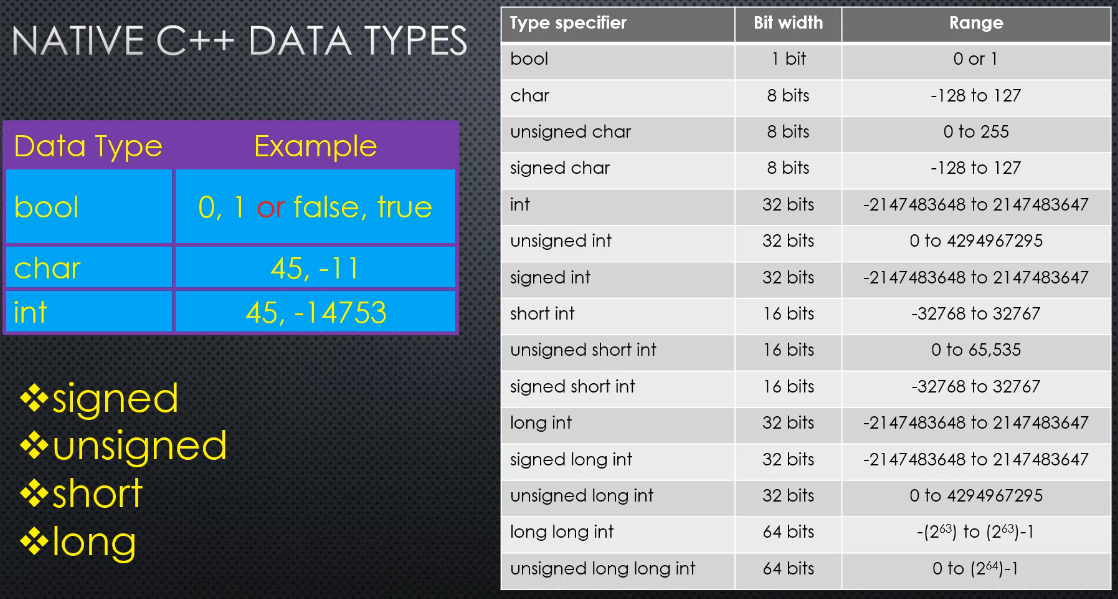
\includegraphics[scale=0.35,frame]{Figures/data_types/data_types_modifiers}
\caption{Data types, modifiers and ranges}
\label{fig:data_types:data_types_modifiers}
\end{figure}

\newpage
\section{Synthesis and Hardware Consideration}

Given some data type, the variables in our code will be mapped to hardware. During this mapping process, some optimization can be made such as eliminating some variables or creating some new intermediate ones.\\ 

Examples are shown in \autoref{fig:data_types:function_example}.

\begin{figure}[h]
\centering
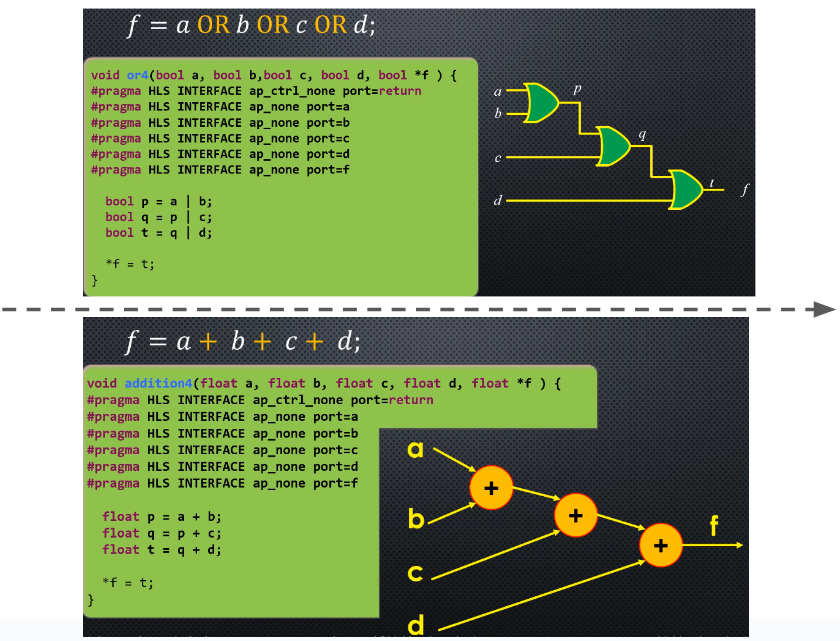
\includegraphics[scale=0.45,frame]{Figures/data_types/function_example}
\caption{Some function example: boolean and arithmetic}
\label{fig:data_types:function_example}
\end{figure}

For the $\mathrm{1}^\mathrm{st}$ system (the boolean function), the circuit can be optimized using the assocaitivity property of \verb|OR| gate, and this result having a system of $t_p \, = \, 3 \delta$ to $t_p \, = \, 2 \delta$ as shown in \autoref{fig:data_types:optim_example}. As for the $\mathrm{2}^\mathrm{nd}$ function (the arithmetic function), the \verb|+| operator will be mapped to adder circuits.

\newpage
\begin{figure}[h]
\centering
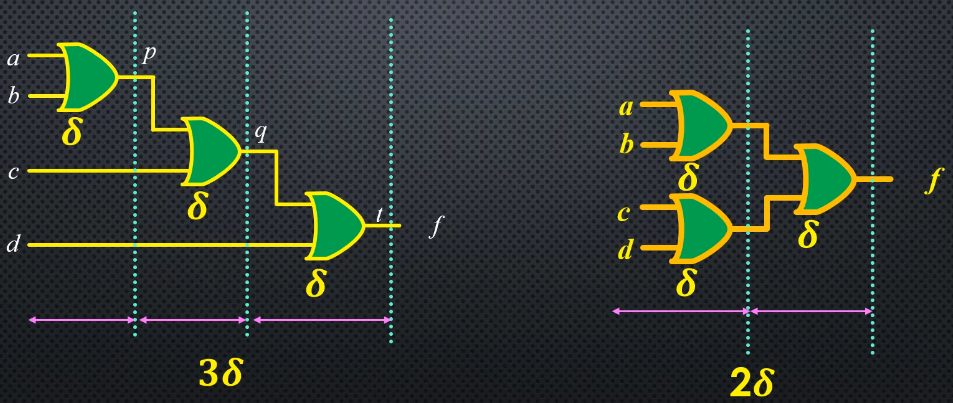
\includegraphics[scale=0.35,frame]{Figures/data_types/optim_example}
\caption{Optimzation of $t_p$}
\label{fig:data_types:optim_example}
\end{figure}


\newpage
\section{Bit Precision}
 
In FPGA programming, it is common to use \textit{arbitrary bit width} with signals, buses,$\cdots$ to have an optimzed solution.
Native \verb|C| data types comes usually with a multiple of 8 (1,8,16,32,$\cdots$), and if we want to implement some circuit let's say a 19 bit multiplier, we can use 32 bit but it's not efficient. That's why the motiviation behind arbitray bit width need.\\

In \verb|HLS|, there exist 2 libraries: 1 for \verb|C| and 1 for \verb|C++|. In this course we focus the one in \verb|C++|. An example is shown in \autoref{fig:data_types:bitwidth_cpp}.

\begin{figure}[h]
\centering
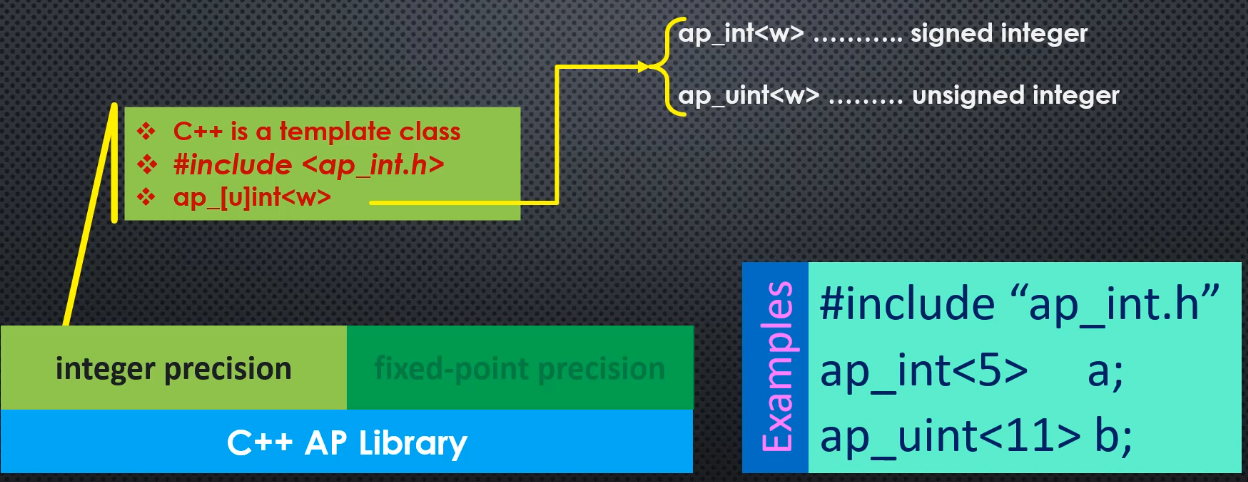
\includegraphics[scale=0.35,frame]{Figures/data_types/bitwidth_cpp}
\caption{Example of C++ library for arbitrary bit width support}
\label{fig:data_types:bitwidth_cpp}
\end{figure}

\todo{Arbitrary width bit in C} \uti{Arbitrary width bit in C:}

\begin{itemize}

\item \textit{To see later the C library, some search about it and some documentation}

\end{itemize}

\newpage
\section{Initialization}

Initialization and assignment is done via class constructor and operator overloading. An example is shown in \autoref{fig:data_types:init_bitwidth_ex}

\begin{figure}[h]
\centering
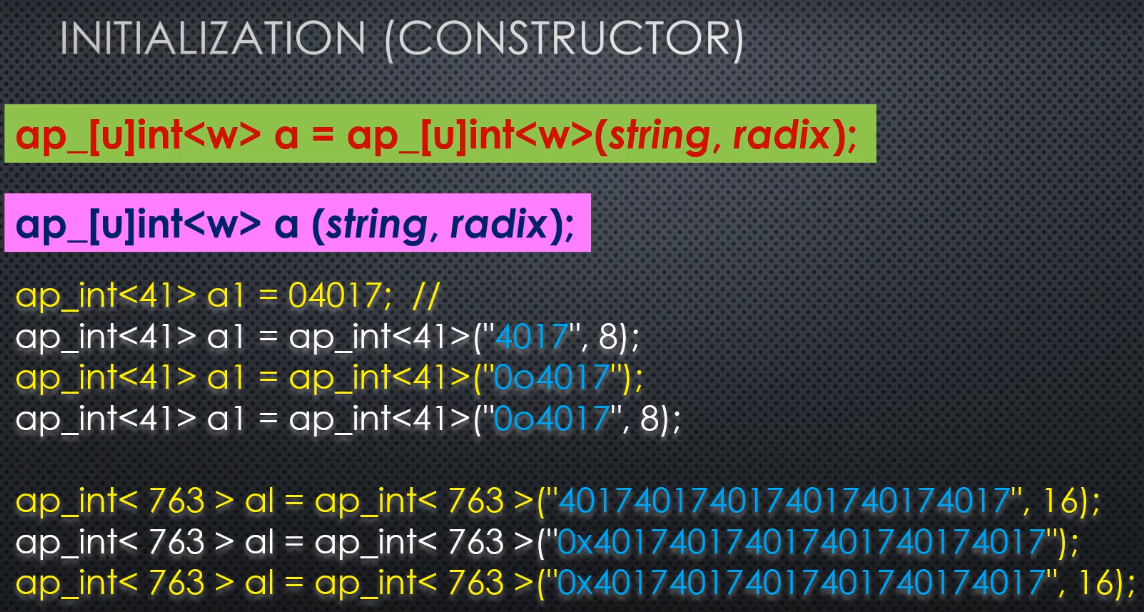
\includegraphics[scale=0.35,frame]{Figures/data_types/init_bitwidth_ex}
\caption{Initialization Example}
\label{fig:data_types:init_bitwidth_ex}
\end{figure}

\begin{itemize}

\item the \verb|ap_int<>| takes 2 argument: a string reprensenting the value and radix (the base), which can be 2,8,10 or 16

	\begin{itemize}
	\item If the $\mathrm{2}^\mathrm{nd}$ argument (the radix) is not provided, the constructor \textit{can infer the base} from the string argument, using prefix \verb|0b| (binary),\verb|0o|(octal), and \verb|0x|(hexadecimal)
	\end{itemize}

\item In $\mathrm{1}^\mathrm{st}$  example in \autoref{fig:data_types:init_bitwidth_ex}, we have 4 different ways of initializing a variable \verb|a1| of width 41 bits with an octal value

	\begin{itemize}
	\item In \verb|C++|, when we intialize a number and put \verb|0| in front, the number is treated as octal (the $\mathrm{1}^\mathrm{st}$ way)
	\end{itemize}

\item In the $\mathrm{2}^\mathrm{nd}$ example in \autoref{fig:data_types:init_bitwidth_ex}, we have 3 ways of initializing variable \verb|al| of width 763 bits with hexadecimal number

\end{itemize}

\newpage
\autoref{fig:data_types:format_printing} presents the ways of printing in the correct base, using \verb|std::oct|,$\cdots$

\begin{figure}[h]
\centering
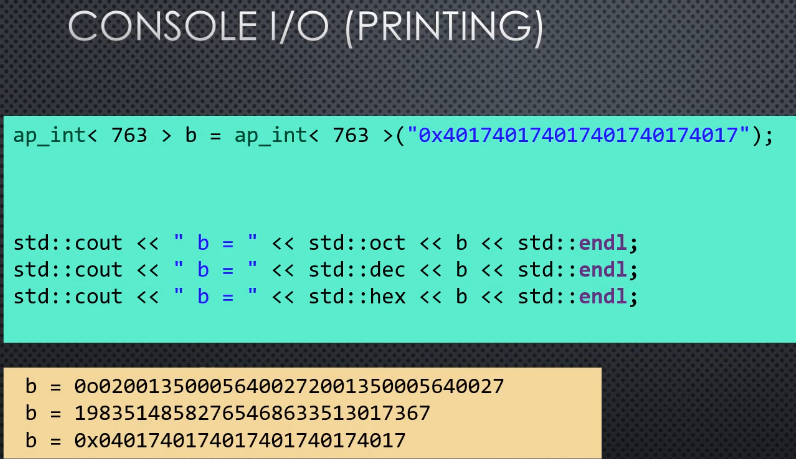
\includegraphics[scale=0.35,frame]{Figures/data_types/format_printing}
\caption{Initialization Example}
\label{fig:data_types:format_printing}
\end{figure}


\newpage
\section{Bit Precision: Assignment}

\autoref{fig:data_types:var_assignment} shows an example of assignment in \verb|HLS| using the \verb|ap_int.h| also.

\begin{figure}[h]
\centering
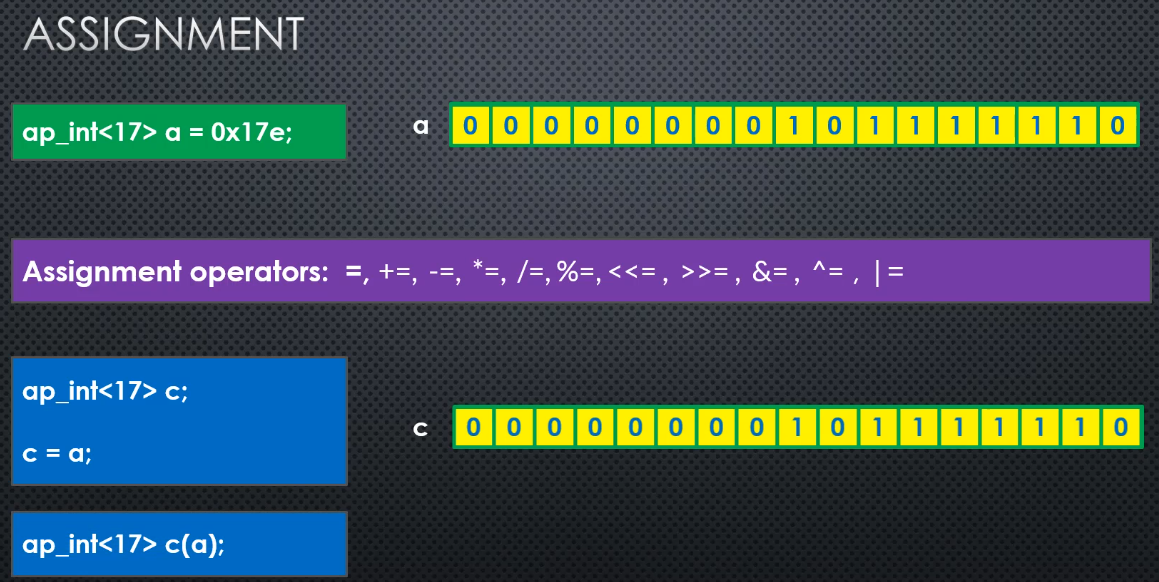
\includegraphics[scale=0.35,frame]{Figures/data_types/var_assignment}
\caption{Assignmnet in HLS}
\label{fig:data_types:var_assignment}
\end{figure}

\begin{itemize}

\item Notice that, a variable can also be assigned to another variable upon its declaration, thanks to the constructors provided by arbitrary precision class template

\end{itemize}

\todo{C++ features and template} \uti{C++ features and template:}

\begin{itemize}

\item \textit{To make a review about C++ programming later , the concept of template, constructor,$\cdots$}

\item \textit{There are many concepts related to constructor and initialization in OOP that I skipped for now in this course}

\item \textit{When I finish my C++ course, I will get back to it later}

\end{itemize}


\newpage
\subsection{Wider and Narrower Assignment}

What happen if we assign some variables having a \textit{different bit width} ? We explore this situation in this section. An example is shown in \autoref{fig:data_types:assignment_types}.


\begin{figure}[h]
\centering
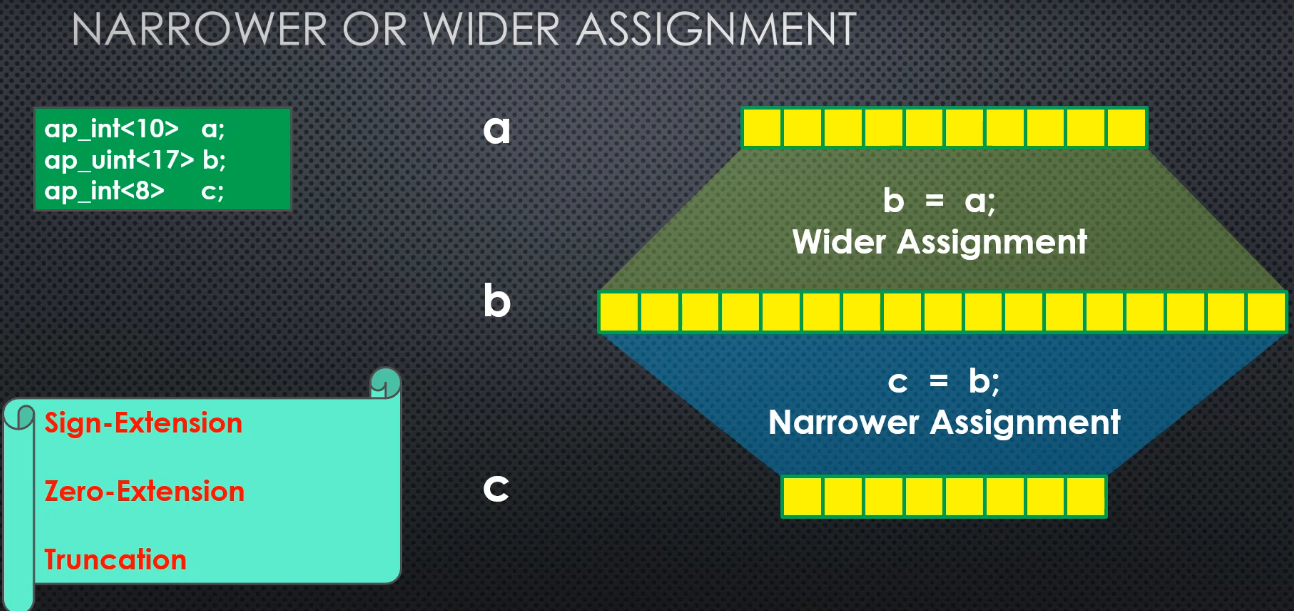
\includegraphics[scale=0.35,frame]{Figures/data_types/assignment_types}
\caption{Assignmnet types: wide and narrow}
\label{fig:data_types:assignment_types}
\end{figure}

\begin{itemize}

\item We have 3 variables: \verb|a|,\verb|b| and \verb|c|

\item \verb|b = a|: we assign \verb|b| to \verb|a|, so the question we need to answer

	\begin{itemize}
	\item this is a \textit{wide assignment} $\leftrightarrow$ what should we do with the extra bits in \verb|b|?
	\end{itemize}

\item \verb|c = b|: we assign \verb|b| to \verb|c|

	\begin{itemize}
	\item This is a \textit{narrow assignment} $\leftrightarrow$ what should we do with missing bits in \verb|b| variable ?
	\end{itemize}

\item The answer to these questions depends on the \textit{signdness}, and we have 3 techniques: sign extension, zero extension, and truncation

\end{itemize}

Let's see how these techniques work.\\

\newpage
\subsection{Sign Extension}

Sign extension is applied when we move from (assing) narrow signed to wider variable.

The value is sign extended to the width of the destination variable, regardless of its its signedness. An example is shown in \autoref{fig:data_types:sign_extension}.


\begin{figure}[h]
\centering
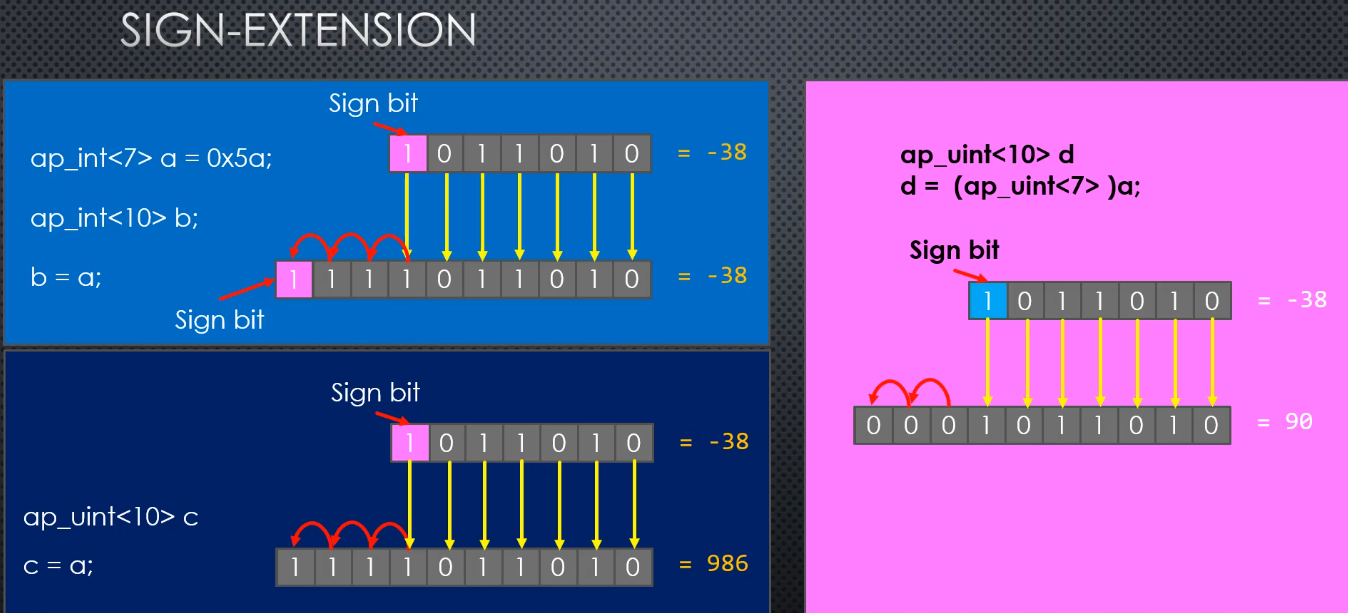
\includegraphics[scale=0.35,frame]{Figures/data_types/sign_extension}
\caption{Sign Extension Example}
\label{fig:data_types:sign_extension}
\end{figure}

\begin{itemize}

\item 2 cases are shown in \autoref{fig:data_types:sign_extension}: \verb|b = a| and \verb|c = a|

	\begin{itemize}
	\item The difference is the type of variable \verb|c| is unsigned integer (\verb|ap_uint()|)
	\end{itemize}

\item In the $\mathrm{1}^\mathrm{st}$ case \verb|b = a|: we fill the extra bits of \verb|b| with the same sign bit of \verb|a|.

\verb|b| holds the same value of \verb|a|

\item In the $\mathrm{2}^\mathrm{nd}$ case \verb|c = a|: also sign bit extension is applied to \verb|c| even though \verb|c| is unisgned integer, and thus \verb|c| will not hold the same value of \verb|a|

\item The $\mathrm{3}^\mathrm{rd}$ example uses the concept of \textit{type casting}: since \verb|a| is a signed integer, we can type caste it to unisgned integer and then assign it to variable \verb|d|

	\begin{itemize}
	\item In this case, signed extension won't happen, and \verb|d| is filled with 0
	\end{itemize}

\end{itemize}

\todo{number representation} \uti{number representation:}

\begin{itemize}

\item \textit{To review number representation and base conversion, because I don't know why c doesn't hold the same value of b or a}	

\end{itemize}

\newpage
\subsection{Zero Extension} 
 
For zero extension, that is filling extra bits with 0, the source variable need to be unsigned. Examples are shown in \autoref{fig:data_types:zero_extension}. 


\begin{figure}[h]
\centering
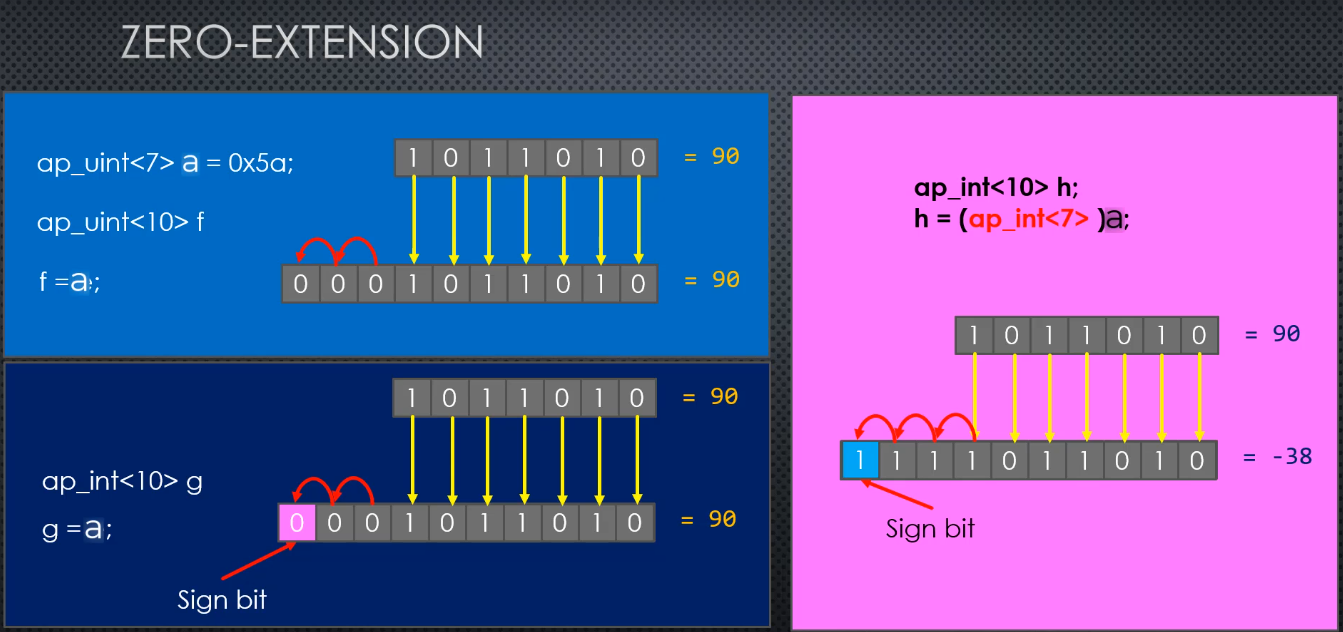
\includegraphics[scale=0.35,frame]{Figures/data_types/zero_extension}
\caption{Zero Extension Example}
\label{fig:data_types:zero_extension}
\end{figure}

\begin{itemize}

\item We have a source variable \verb|a| which is unsigned

\item we have 2 operation: 

	\begin{itemize}
	\item \verb|f = a|, \verb|f| is also unisgned
	
	\item \verb|g = a|. \verb|g| is signed
	\end{itemize}

\item In the $\mathrm{3}^\mathrm{rd}$ operation  where we have variable \verb|h| and type casting is used, the value \verb|a| is changed during assignment from 90 to -38

\end{itemize}

\newpage
\subsection{Truncation}

Now we take the $\mathrm{2}\mathrm{nd}$ case, that is moving from wider to narrow variable, which is known as truncation.

\begin{figure}[h]
\centering
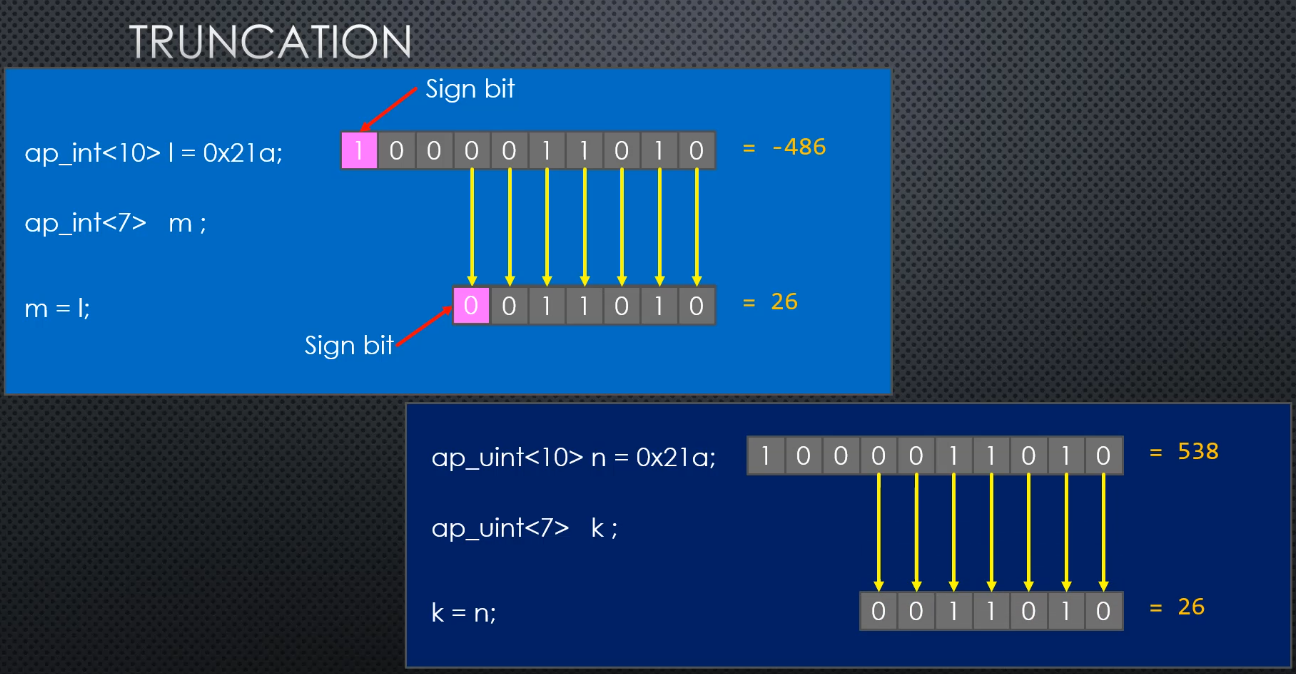
\includegraphics[scale=0.35,frame]{Figures/data_types/truncation}
\caption{Truncation Example}
\label{fig:data_types:truncation}
\end{figure}

\begin{itemize}

\item In truncation, MSB is lost, and no special treatment for signed bit, which may lead to unexpected behavior

\end{itemize}

\newpage
\section{Bit Level Operation} 

Now we introduce several bit level operation. 


\subsection{Concatenation}

\begin{figure}[h]
\centering
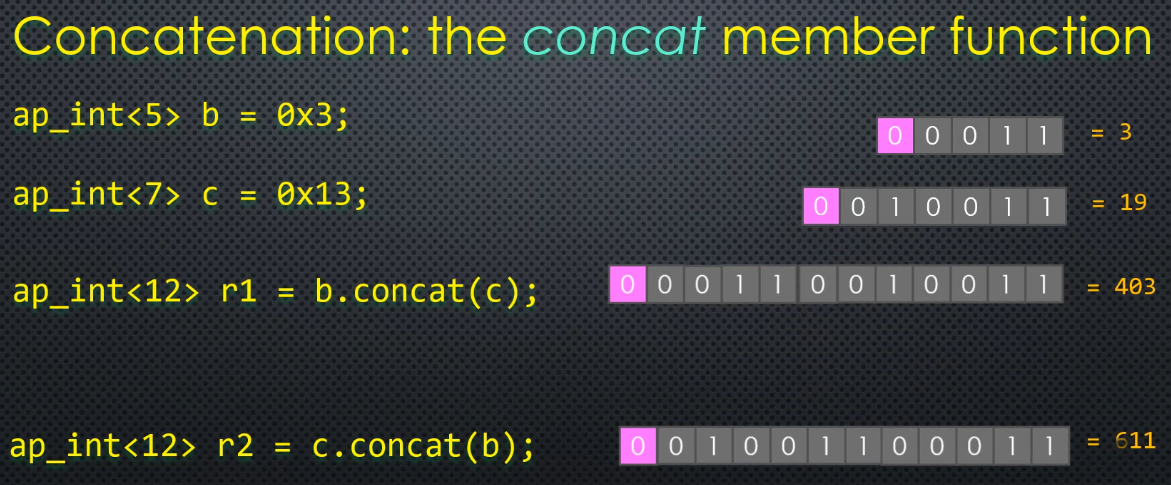
\includegraphics[scale=0.35,frame]{Figures/data_types/concat}
\caption{Concatenation}
\label{fig:data_types:concat}
\end{figure} 
 
\begin{itemize}

\item \verb|b.concat(c)|: \verb|b| will be in the upper part, and \verb|c| is in the lower part

\end{itemize} 
 
Concatenation can also be done using the comma overloaded operator as shown in \autoref{fig:data_types:concat_comma}.
 
\begin{figure}[h]
\centering
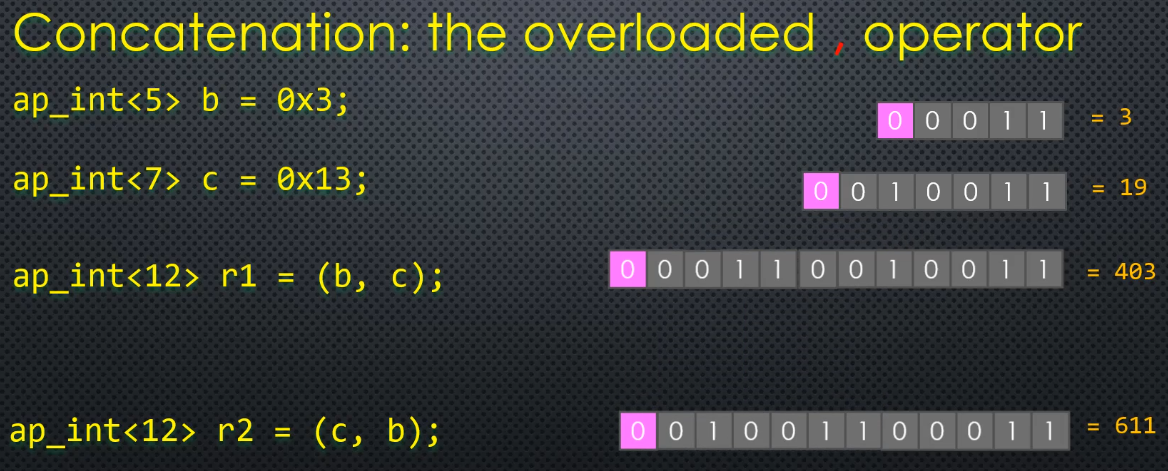
\includegraphics[scale=0.35,frame]{Figures/data_types/concat_comma}
\caption{Concatenation}
\label{fig:data_types:concat_comma}
\end{figure}  
 
\newpage  
\subsection{Bit Selection} 
 
Bit selection can be done using the overlaoded \verb|[]| operator as shown in \autoref{fig:data_types:bit_selection}.

\begin{figure}[h]
\centering
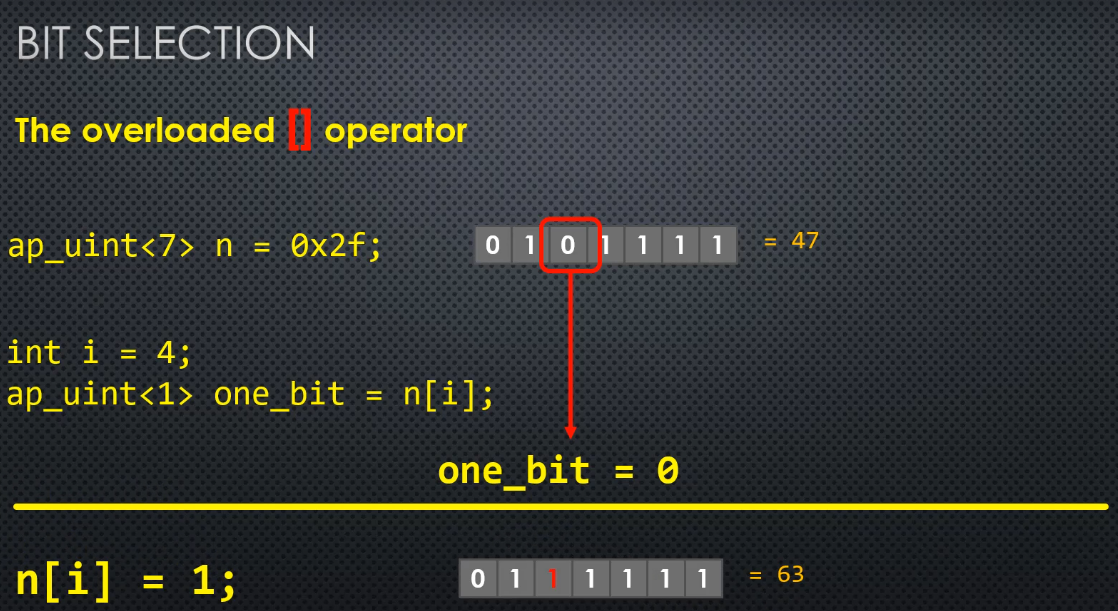
\includegraphics[scale=0.35,frame]{Figures/data_types/bit_selection}
\caption{Bit Selection}
\label{fig:data_types:bit_selection}
\end{figure} 
 
\newpage 
\subsection{Range Selection} 
 
Selecting a range of consecutive bits can be done the \verb|range()| function as shown in \autoref{fig:data_types:range_bits}.

\begin{figure}[h]
\centering
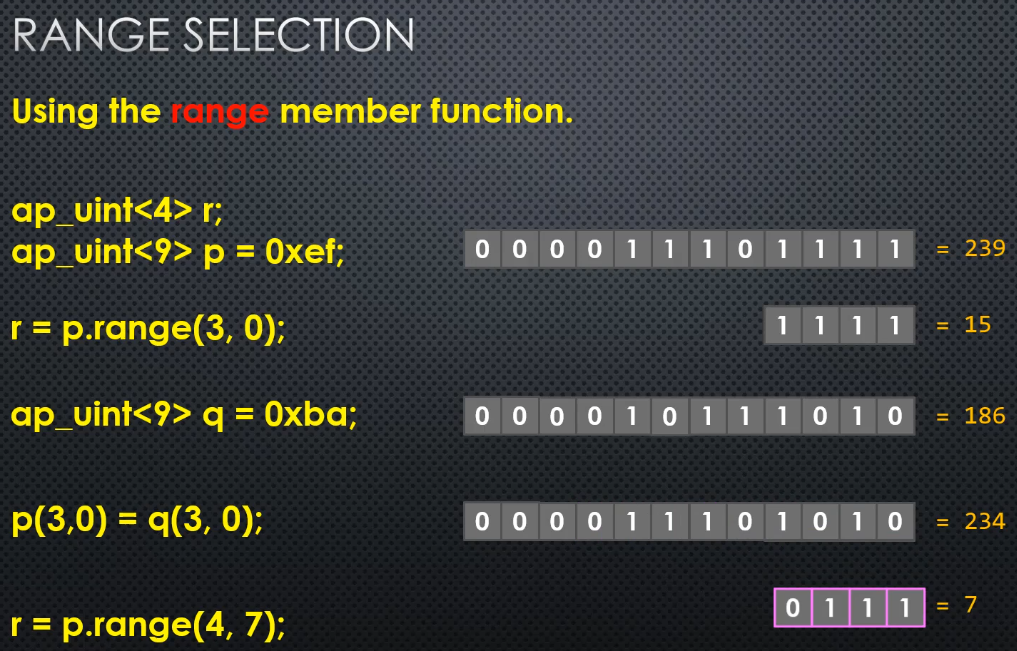
\includegraphics[scale=0.35,frame]{Figures/data_types/range_bits}
\caption{Selecing a range of bits}
\label{fig:data_types:range_bits}
\end{figure}
 
 
 \uti{Range bits:} \todo{Range bits}

\begin{itemize}

\item \textit{There are some mistake int the $\mathrm{2}^\mathrm{nd}$ example of \autoref{fig:data_types:range_bits}}

\item \textit{I will search an example for the correct use of arguments}

\end{itemize}

\newpage
\subsection{Bitwise Logical Operator}

We continue exploring bitwise operations with logical operator on a bitlevel as shown in \autoref{fig:data_types:bitwise_operations}.

\begin{figure}[h]
\centering
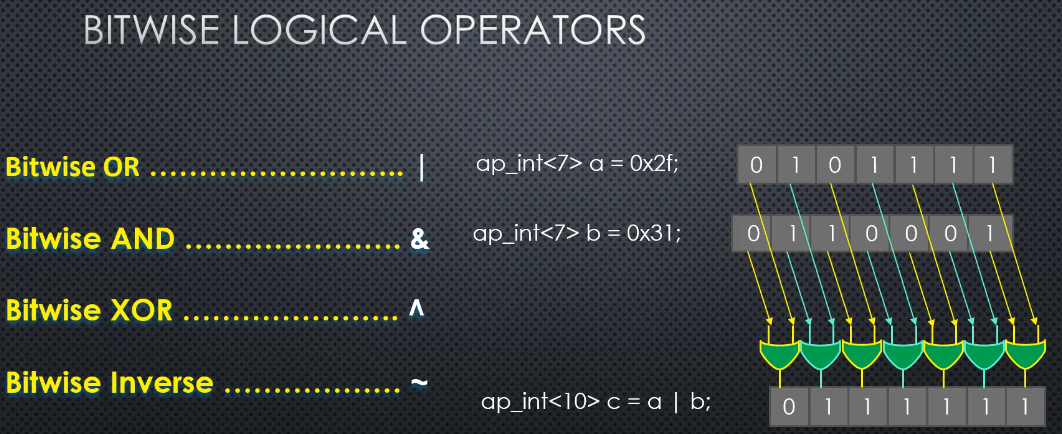
\includegraphics[scale=0.35,frame]{Figures/data_types/bitwise_operations}
\caption{Bitwise Operation Example}
\label{fig:data_types:bitwise_operations}
\end{figure}

\begin{itemize}

\item Bitwise logical operators all return a value with a width
that is the maximum of the widths of the two operands

\item They are treated as unsigned if and only if both operands are unsigned

\item Otherwise, it is of a signed type, sign-extension (or zero-padding) may occur, based on the signedness of the expression, not the destination variable

\end{itemize}

\uti{Bitwise logical operator:} \todo{Bitwise logical operator}

\begin{itemize}

\item \textit{To make sure of this concepts of max width return, and zero extension, because in emebdedded C I don't think I encountered such concepts before}

\end{itemize}

\newpage
\subsection{Reduced Logical Function}

Reduced functions apply a given operator to all bits of an arbitrary precision value and return a one-bit result. An example is shown in \autoref{fig:data_types:reduced_logical_function}.

\begin{figure}[h]
\centering
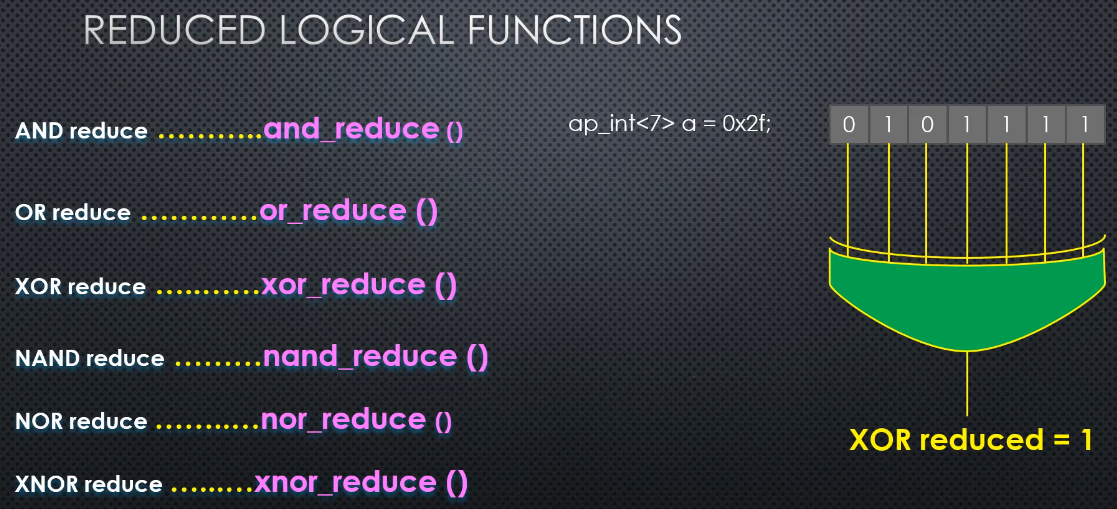
\includegraphics[scale=0.35,frame]{Figures/data_types/reduced_logical_function}
\caption{Reduced Logical Function}
\label{fig:data_types:reduced_logical_function}
\end{figure}

\uti{Reduced Logical Function:} 

\todo{Reduced Logical Function}

\begin{itemize}

\item \textit{There are no mentions for the rules of such operation, to be seen later}

\end{itemize}

\newpage
\subsection{Test,Set Clear}

Set,reset and test function example are shown in \autoref{fig:data_types:set_reset_test}.

\begin{figure}[h]
\centering
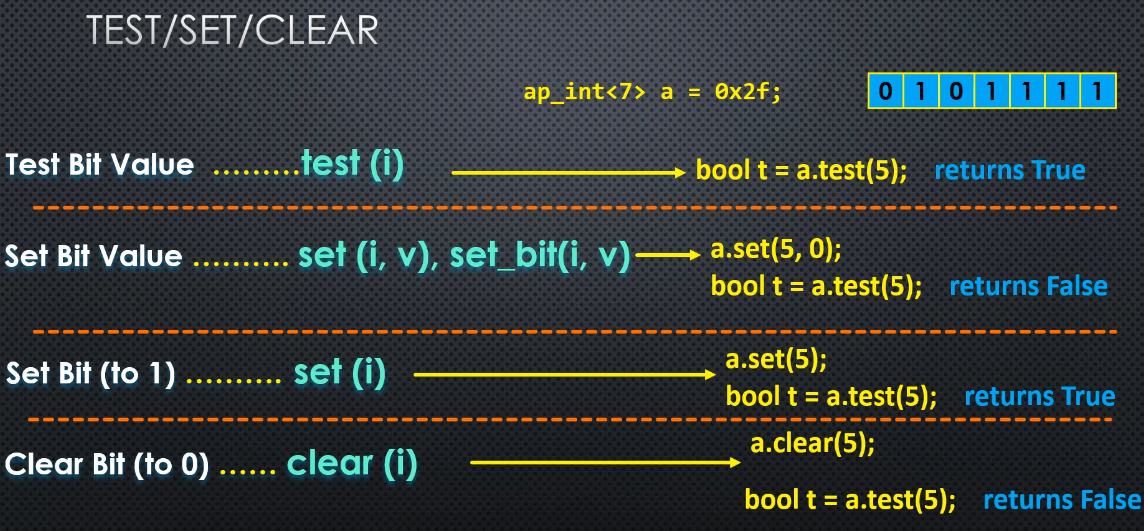
\includegraphics[scale=0.35,frame]{Figures/data_types/set_reset_test}
\caption{Test,Set and Clear}
\label{fig:data_types:set_reset_test}
\end{figure}


\newpage
\subsection{Bit Shift and Rotate}

Now we move to bit shifting operations. Shift operation are performed right and left direction as shown in \autoref{fig:data_types:bit_shift}.

\begin{figure}[h]
\centering
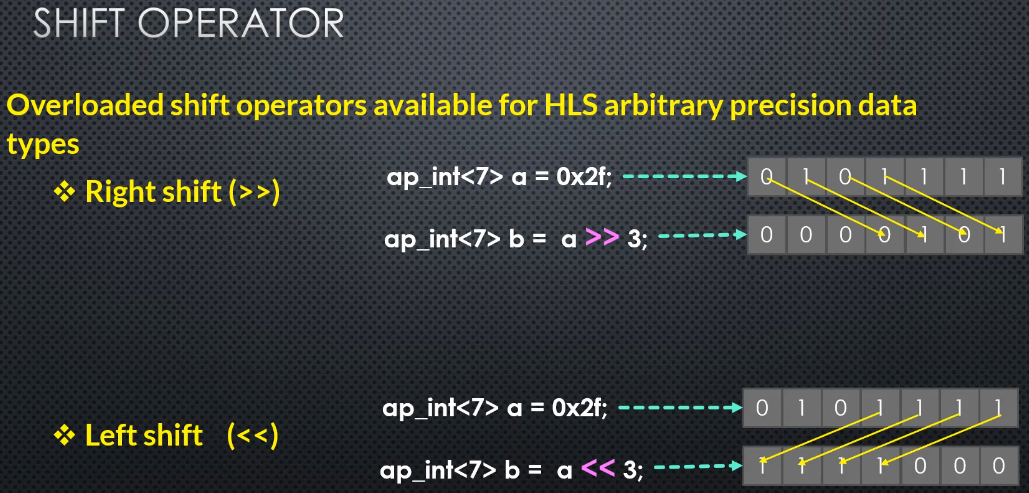
\includegraphics[scale=0.35,frame]{Figures/data_types/bit_shift}
\caption{Bit shift operation}
\label{fig:data_types:bit_shift}
\end{figure}

Also in \verb|HLS| we have some functions to do some rotation to the bits, also in left and right as shown in \autoref{fig:data_types:bit_rotate}.

\begin{figure}[h]
\centering
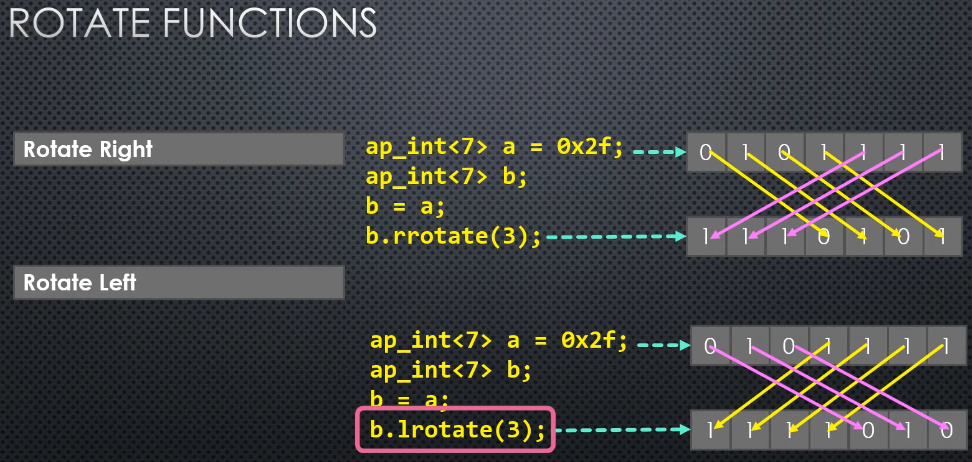
\includegraphics[scale=0.35,frame]{Figures/data_types/bit_rotate}
\caption{Bit rotation}
\label{fig:data_types:bit_rotate}
\end{figure}








\chapter{Decision Making}

\section{Introduction}

Conditional statements and decision making plays an important role in algorithmic design. In this chapter, we see how an condition statment can be implemented, and what is the corresponding hardware for such a task.

\section{Recap}

Recall that a condition is usually implemented in software as \verb|if-else| as shown in \autoref{fig:conditions:condition_soft}.


\begin{figure}[h]
\centering
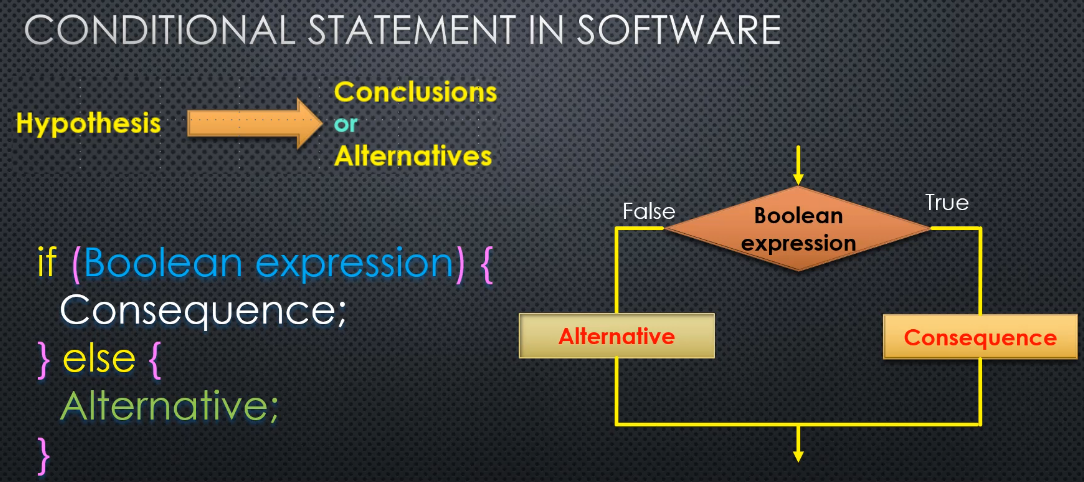
\includegraphics[scale=0.35,frame]{Figures/conditions/condition_soft}
\caption{Condition in software}
\label{fig:conditions:condition_soft}
\end{figure}

\begin{itemize}

\item We have some condition define by some boolean expression

\item if the condition is true consequence is selected else the alternative is selected

\end{itemize}

\newpage
As hardware, and \verb|if-else| statement can be modeled using a switch as shown in 

\begin{figure}[h]
\centering
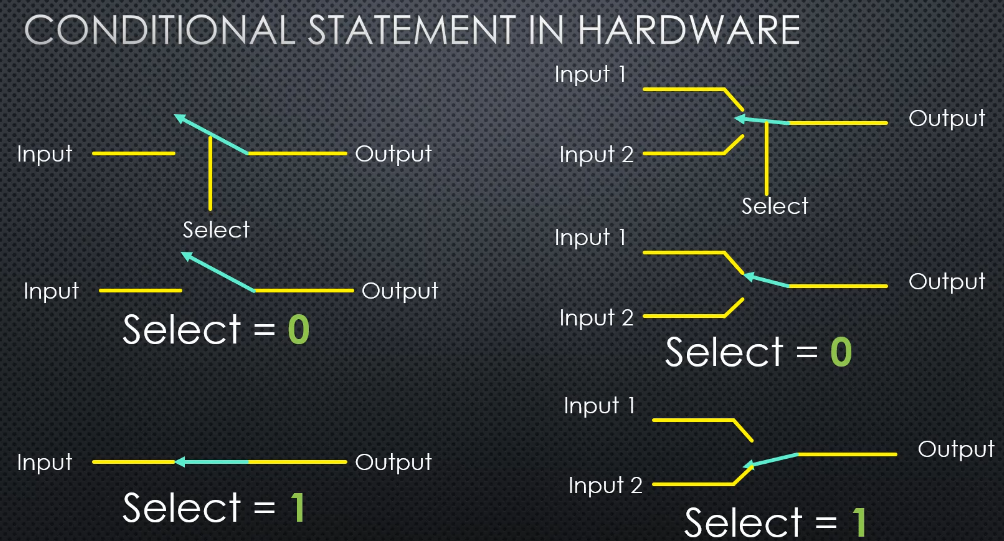
\includegraphics[scale=0.35,frame]{Figures/conditions/condition_hard_switch}
\caption{Condtion modeled using a switch}
\label{fig:conditions:condition_hard_switch}
\end{figure}

\begin{itemize}

\item In the special case we have switch to select between 1 input

	\begin{itemize}
	\item This correspond to a special \verb|if| where we have no  \verb|else| condition
	\end{itemize}

\item Then the general case where switch is selecting between multiple inputs

\end{itemize}



\newpage
\section{Multiplexer}

To impelement conditions using logic gates, usually we use a MUX circuit as shown in \autoref{fig:conditions:MUX}.

\begin{figure}[h]
\centering
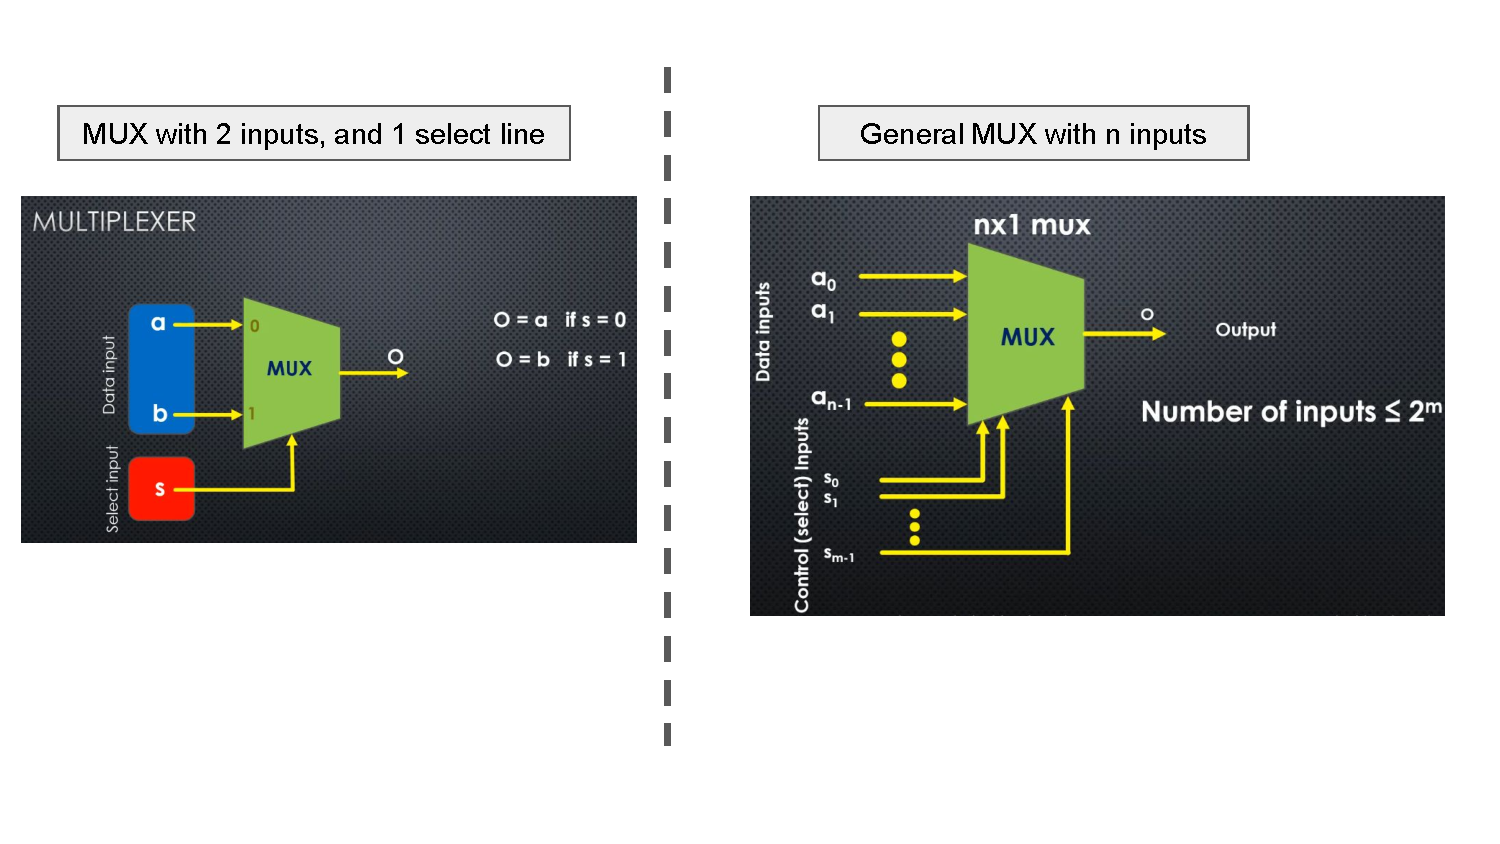
\includegraphics[scale=0.65,frame]{Figures/conditions/MUX}
\caption{Multiplexer}
\label{fig:conditions:MUX}
\end{figure}

\begin{itemize}

\item In the right hand side, we have the special case MUX where we have 1 select line to select between inputs

\item Then we have the generalize case where we have $m$ select line to select between $n$ inputs

\end{itemize}

\newpage
\subsection{Generalized Mux and if-else}

Now in real applications, the MUX shown in \autoref{fig:conditions:MUX} doesn't come in straightforward manner, we usually apply some preprocessing steps on the selection line or even in the input section, to have the appropriate output.

\begin{figure}[h]
\centering
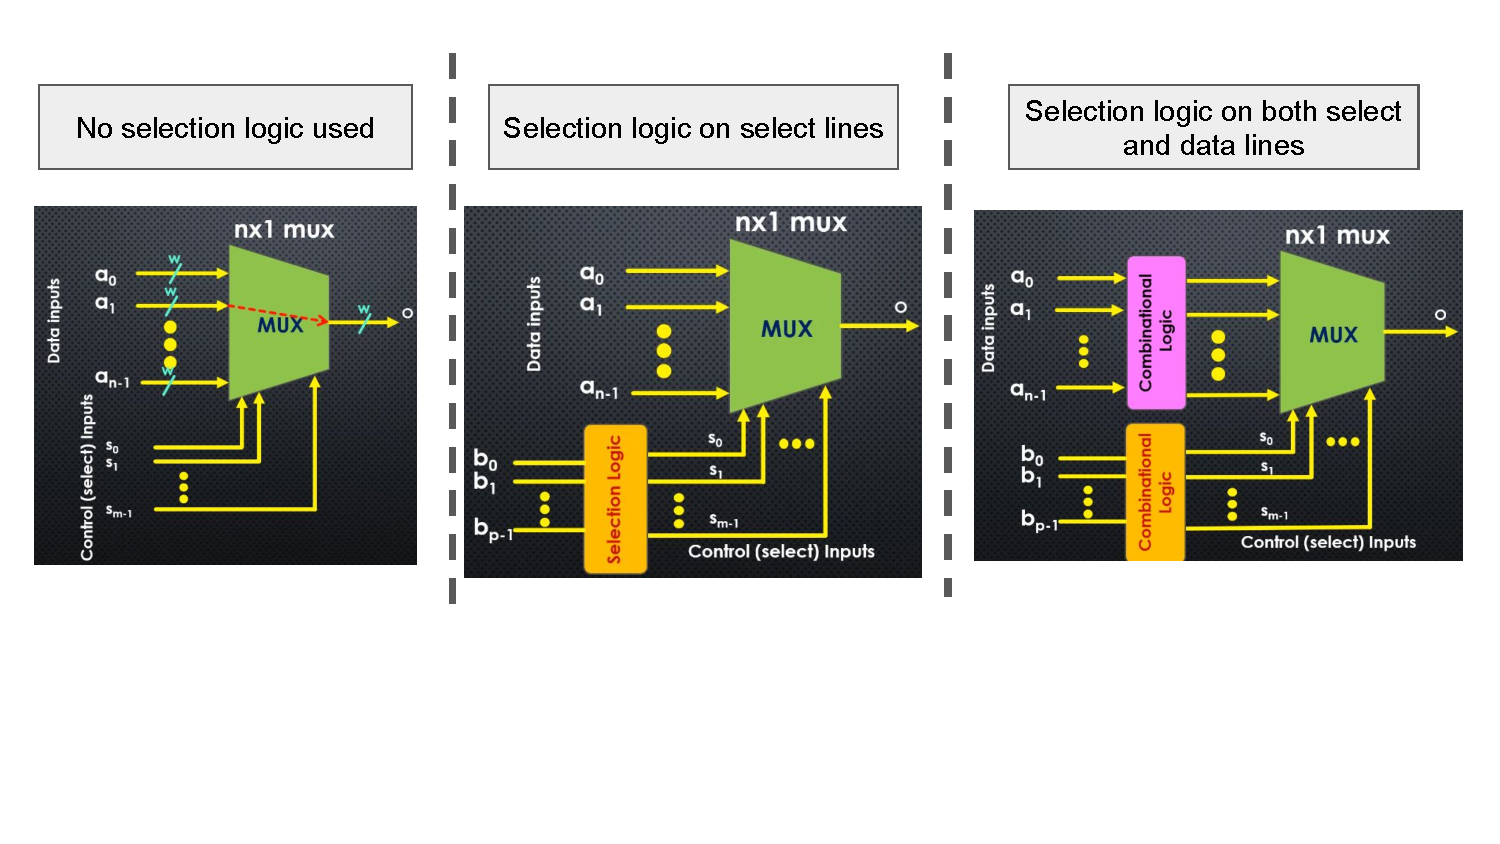
\includegraphics[scale=0.65,frame]{Figures/conditions/generalized_mux}
\caption{Generalized Multiplexer Circuits}
\label{fig:conditions:generalized_mux}
\end{figure}


We see in this section some examples to see the mapping between \verb|if-else| conditions and the corresponding MUX circuit.

\newpage
$\mathrm{1}^\mathrm{st}$ example is presented in \autoref{fig:conditions:if_else_ex_1}

\begin{figure}[h]
\centering
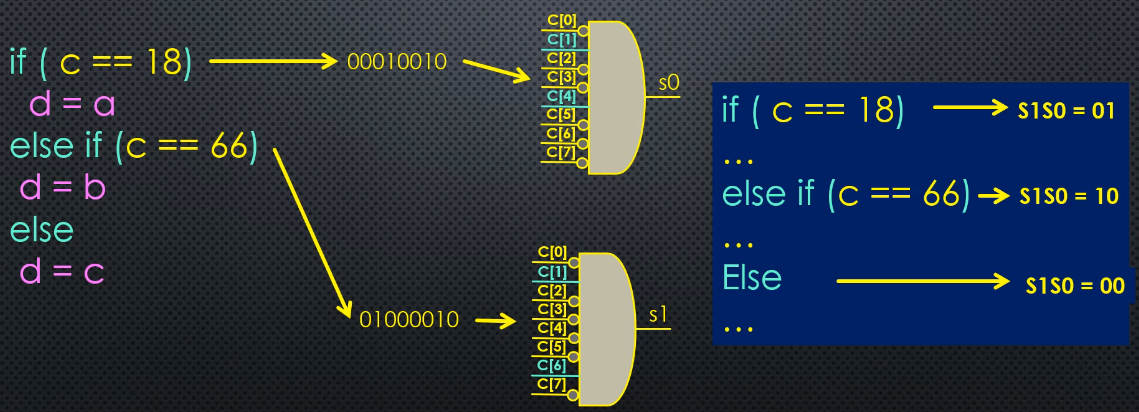
\includegraphics[scale=0.35,frame]{Figures/conditions/if_else_ex_1}
\caption{if esle example}
\label{fig:conditions:if_else_ex_1}
\end{figure}

\begin{itemize}

\item We have on the right hand side some \verb|if-else| statment

	\begin{itemize}
	\item \verb|d| is output, \verb|a|,\verb|b| and \verb|c| inputs
	
	\item \verb|c| is also present the role of the selection line
	\end{itemize}

\item Here we need to select line $s_0$ and $s_1$ since we have 4 inputs

\item the conditions \verb|c==18| and \verb|c==66| are mapped to some \verb|AND| gate, each with their corresponding binary values

\item When $s_1 \, s_0 \, = \, 01$ condition \verb|c==18| is validate, hence \verb|a| is selected and mapped to output \verb|d|, and same logic with other values

\end{itemize}

The corresponding MUX circuit of \autoref{fig:conditions:if_else_ex_1} is shown in \autoref{fig:conditions:if_else_ex_1_circuit}.

\begin{figure}[h]
\centering
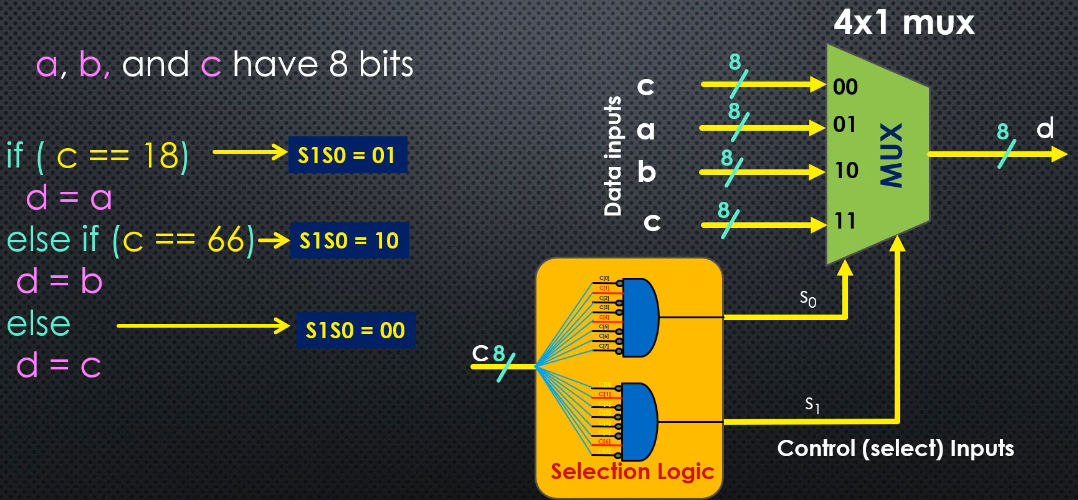
\includegraphics[scale=0.35,frame]{Figures/conditions/if_else_ex_1_circuit}
\caption{if esle example with MUX circuit}
\label{fig:conditions:if_else_ex_1_circuit}
\end{figure}

\newpage
$\mathrm{2}^\mathrm{nd}$ example is presented in \autoref{fig:conditions:if_else_ex_2}, where combinational logic are also presented on the input line section, since we have some preprocessing before passing inputs to output line \verb|d|

\begin{figure}[h]
\centering
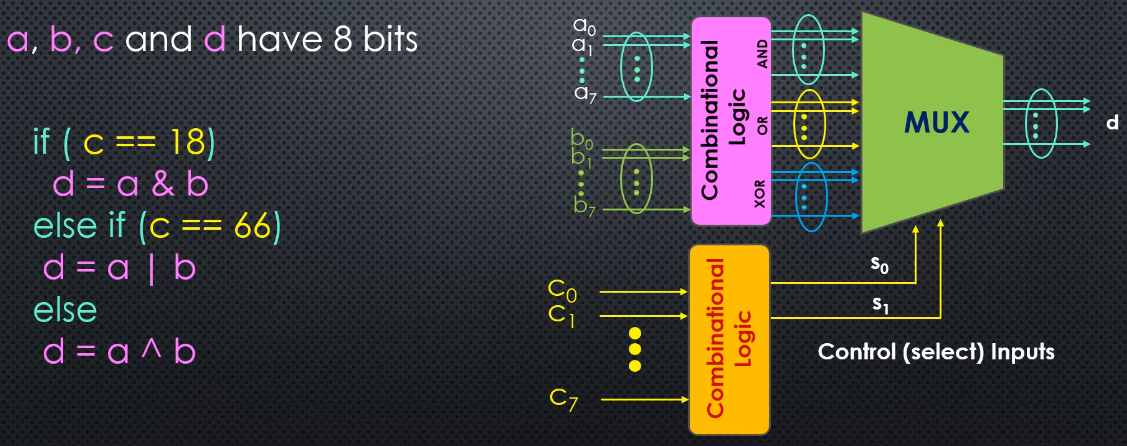
\includegraphics[scale=0.35,frame]{Figures/conditions/if_else_ex_2}
\caption{if esle example: combinational circuit on both lines}
\label{fig:conditions:if_else_ex_2}
\end{figure}

\newpage
\subsection{Quiz}

\underline{Quiz 1:} what is the hardware implementation that implement decision making process shown in \autoref{fig:conditions:quiz_if_else}?

\begin{figure}[h]
\centering
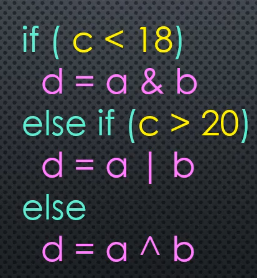
\includegraphics[scale=0.45,frame]{Figures/conditions/quiz_if_else}
\caption{Quiz 1}
\label{fig:conditions:quiz_if_else}
\end{figure}

\underline{Solution Quiz 1:}

\begin{figure}[h]
\centering
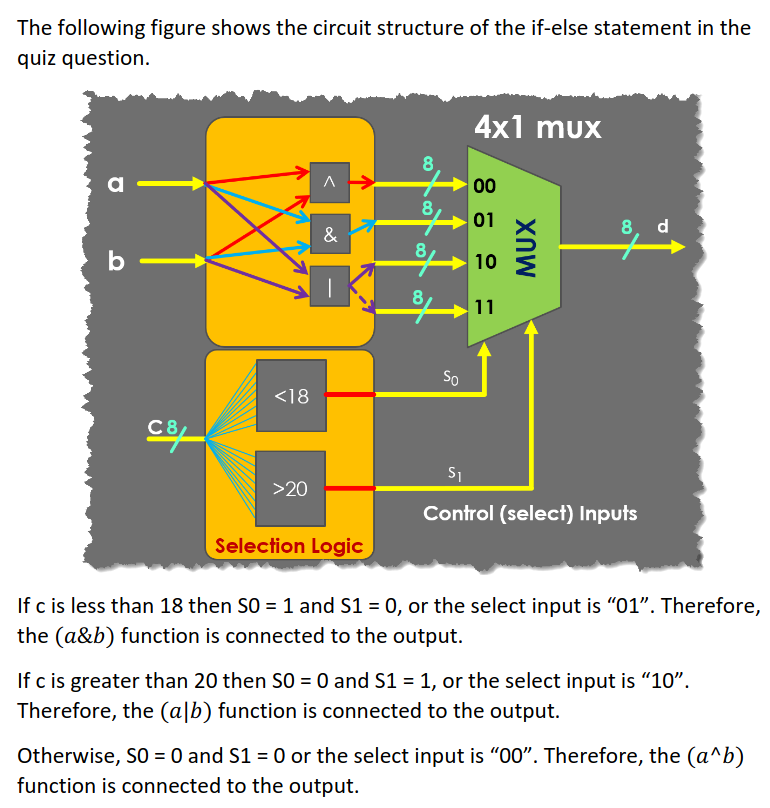
\includegraphics[scale=0.40,frame]{Figures/conditions/quiz_if_else_sol}
\caption{Quiz 1 Solution}
\label{fig:conditions:quiz_if_else_sol}
\end{figure}

\newpage
\underline{Quiz 2:} Draw the structure of the combinational circuit that can implement the \verb|HLS| code shown in \autoref{fig:conditions:quiz_switch_case}.

\begin{figure}[h]
\centering
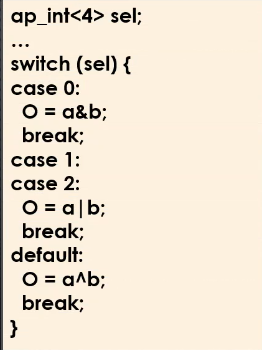
\includegraphics[scale=0.35,frame]{Figures/conditions/quiz_switch_case}
\caption{Quiz 2}
\label{fig:conditions:quiz_switch_case}
\end{figure}

\underline{Solution Quiz 2:}

\begin{figure}[h]
\centering
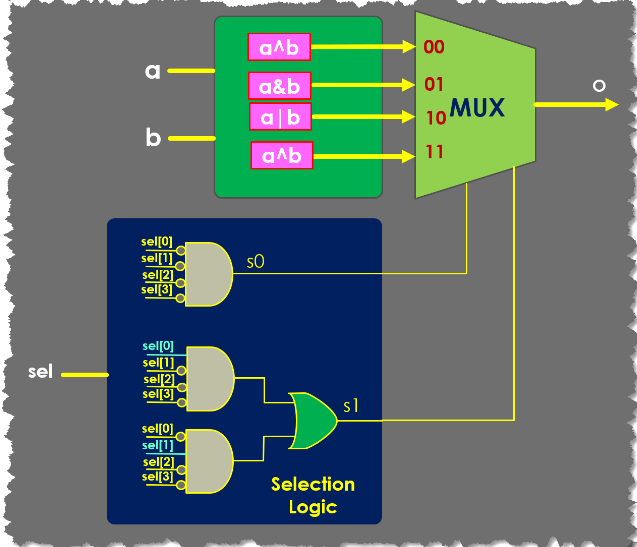
\includegraphics[scale=0.45,frame]{Figures/conditions/quiz_switch_case_sol}
\caption{Quiz 2 Solution}
\label{fig:conditions:quiz_switch_case_sol}
\end{figure}


\newpage
\section{Coders}

Now we move to coders circuit, that is encoder and decoder.

Recall that encoder is a circuit which transforms data from one shape to the other for various reason (security,compression,$\cdots$). Decoder does the opposite, that is retreive the original data from the coded data. In other words, encoders and decoders are circuit \tbi{change the forme of the data}.


\begin{figure}[h]
\centering
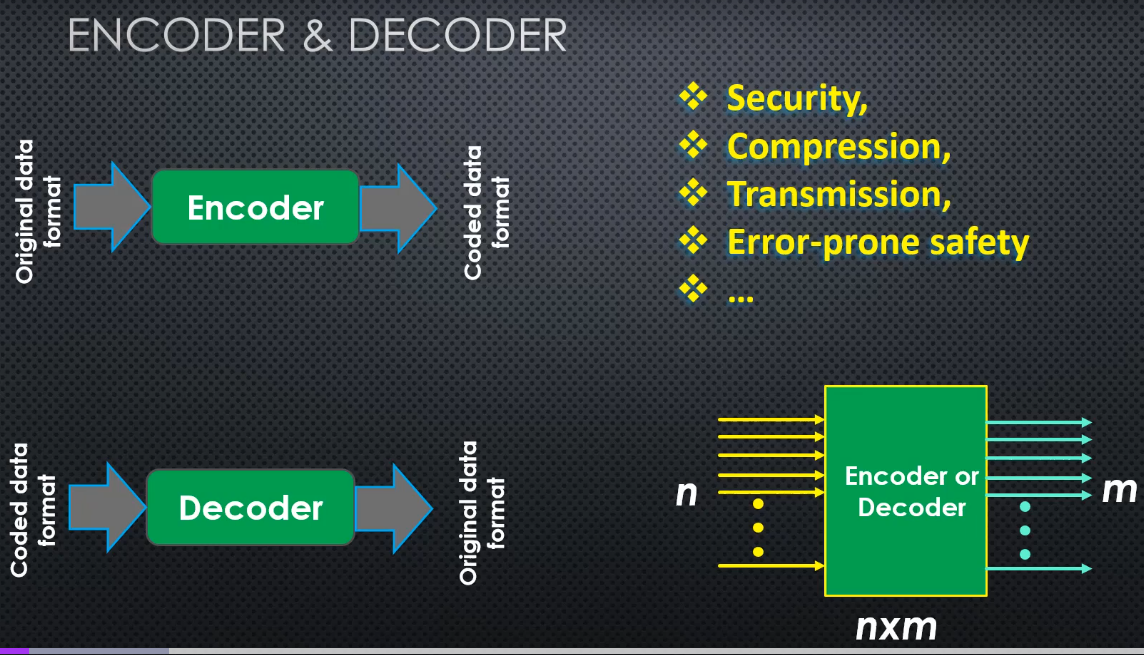
\includegraphics[scale=0.40,frame]{Figures/conditions/coders}
\caption{Encoder and Decoder}
\label{fig:conditions:coders}
\end{figure}


In general, coders circuit take $n$ input bits and generate $m$ output bits.

\newpage
\subsection{Examples}

As example, \autoref{fig:conditions:4_by_2_encoder} presents a 4 by 2 encoder. The encoder alwyas encode the input data \tbi{into a compact form}, so the number of output is less than the number of inputs.

\begin{figure}[h]
\centering
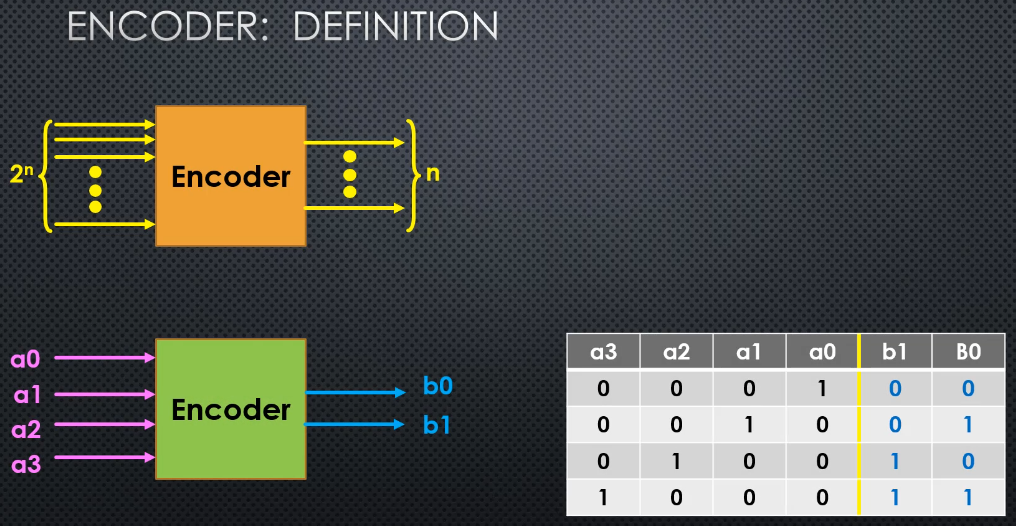
\includegraphics[scale=0.40,frame]{Figures/conditions/4_by_2_encoder}
\caption{4 by 2 Encoder}
\label{fig:conditions:4_by_2_encoder}
\end{figure}

The opposite of system in \autoref{fig:conditions:4_by_2_encoder} is presented in \autoref{fig:conditions:2_by_4_decoder}. Notice that binary input represents the position index of the 1 in output. For example last row , binary input 11 (equivalent to 3 in base 10) is the index of 1 in $b_0 \,b_1 \, b_2 \, b_3$

\begin{figure}[h]
\centering
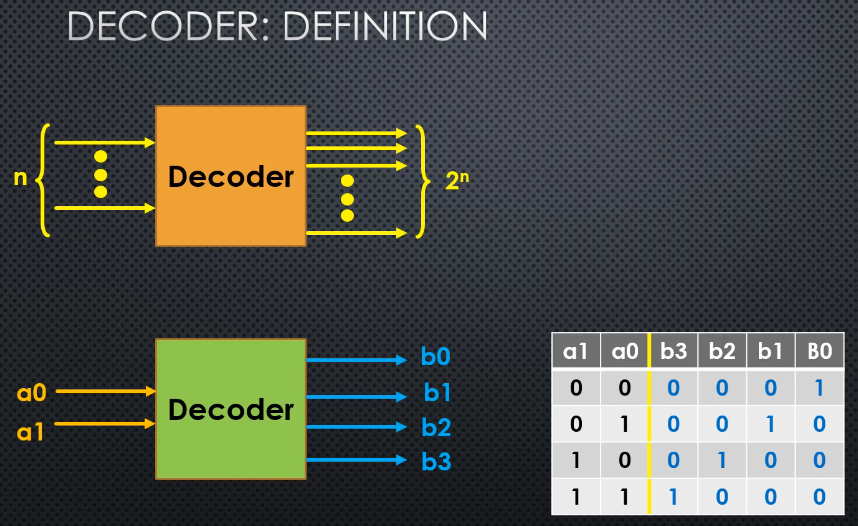
\includegraphics[scale=0.40,frame]{Figures/conditions/2_by_4_decoder}
\caption{2 by 4 Decoder}
\label{fig:conditions:2_by_4_decoder}
\end{figure}

\newpage
\subsection{Decoder in HLS}

An \verb|switch| case can be used to impelement a decoder or encoder in \verb|HLS|. The \verb|HLS| implementation of example of \autoref{fig:conditions:2_by_4_decoder} (the 2 by 4 decoder) is shown in \autoref{fig:conditions:2_by_4_decoder_hls}.


\begin{figure}[h]
\centering
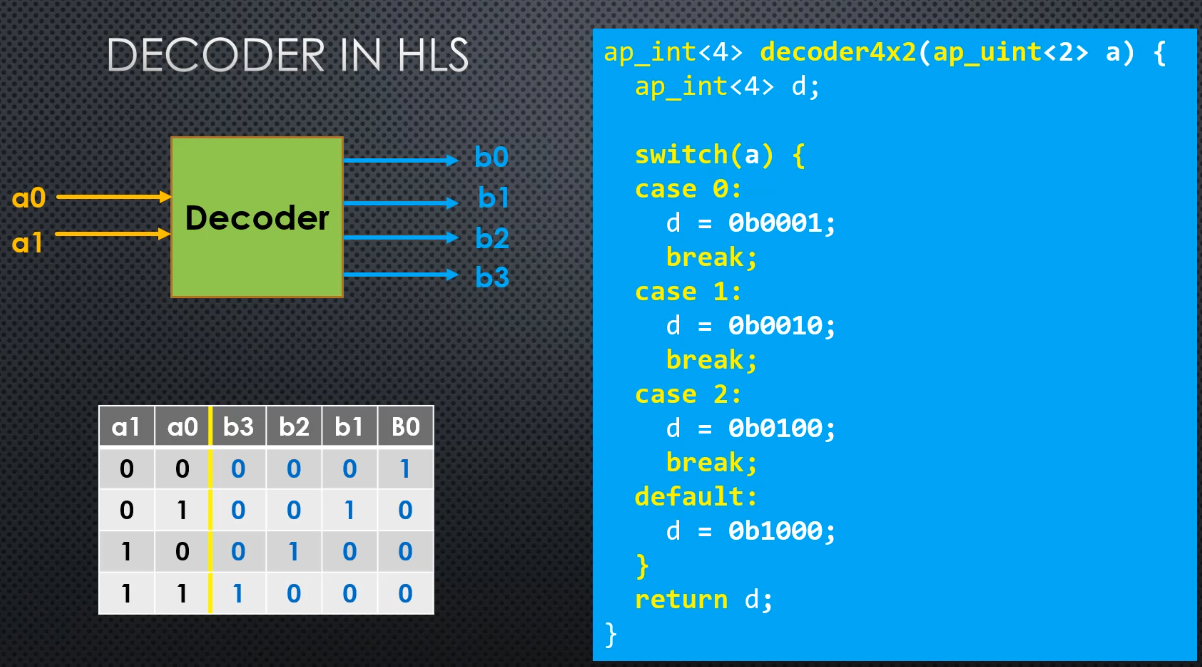
\includegraphics[scale=0.33,frame]{Figures/conditions/2_by_4_decoder_hls}
\caption{HLS impelemtation for 2 by 4 Decoder}
\label{fig:conditions:2_by_4_decoder_hls}
\end{figure}

The \verb|HLS| tool can the sythesise the code. A MUX can be used to implement the \verb|switch| case for the decoder as shown in \autoref{fig:conditions:2_by_4_decoder_hls_synthesis}.

\begin{figure}[h]
\centering
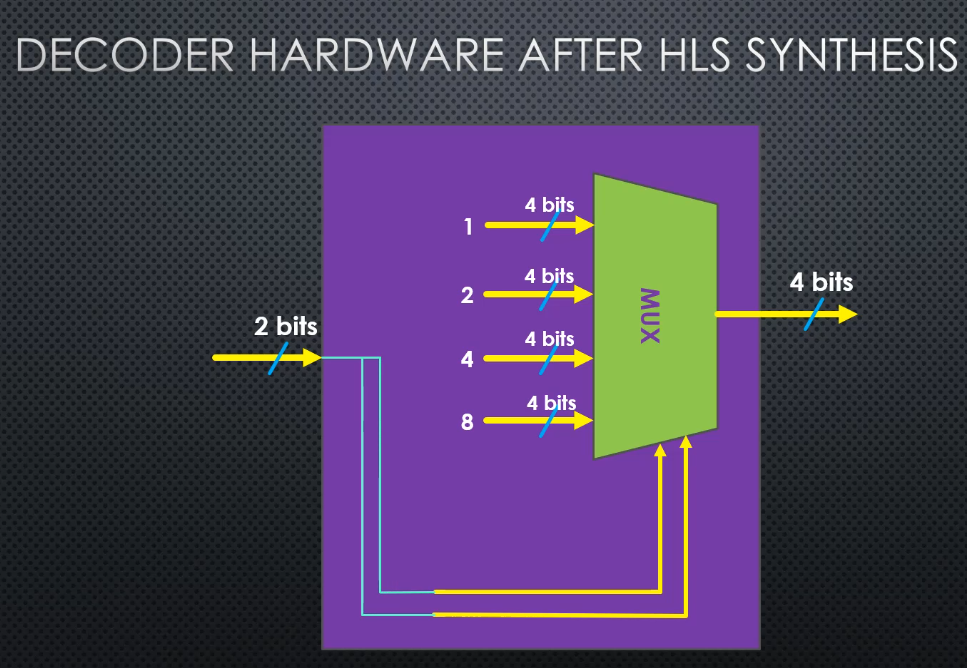
\includegraphics[scale=0.30,frame]{Figures/conditions/2_by_4_decoder_hls_synthesis}
\caption{HLS Synthesis for the 2 by 4 Decoder}
\label{fig:conditions:2_by_4_decoder_hls_synthesis}
\end{figure}


\newpage
\subsection{Quiz}

\underline{Quiz Decoder:} use a \verb|switch| case statement to describe and $8 \times 3$ encoder circuit.\\

\underline{Solution:}

\begin{figure}[h]
\centering
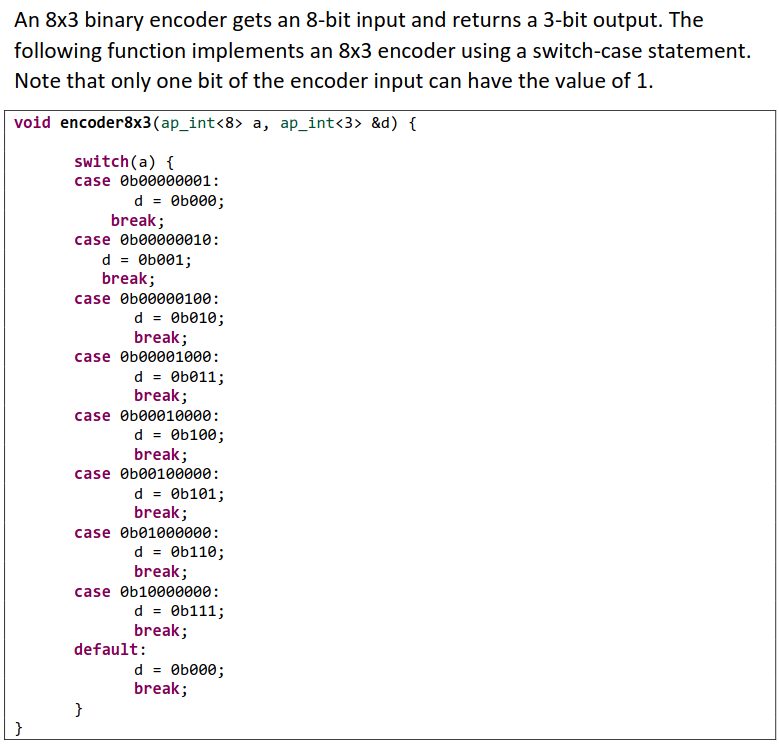
\includegraphics[scale=0.50,frame]{Figures/conditions/quiz_decoder}
\caption{Solution for quiz decoder}
\label{fig:conditions:quiz_decoder}
\end{figure}













\chapter{Seven Segment Dsiplay}

\section{Introduction}

Seven segement display are one of the classical display units which are present in many electronics systems as shown in \autoref{fig:seven_seg:applications}.

\begin{figure}[h]
\centering
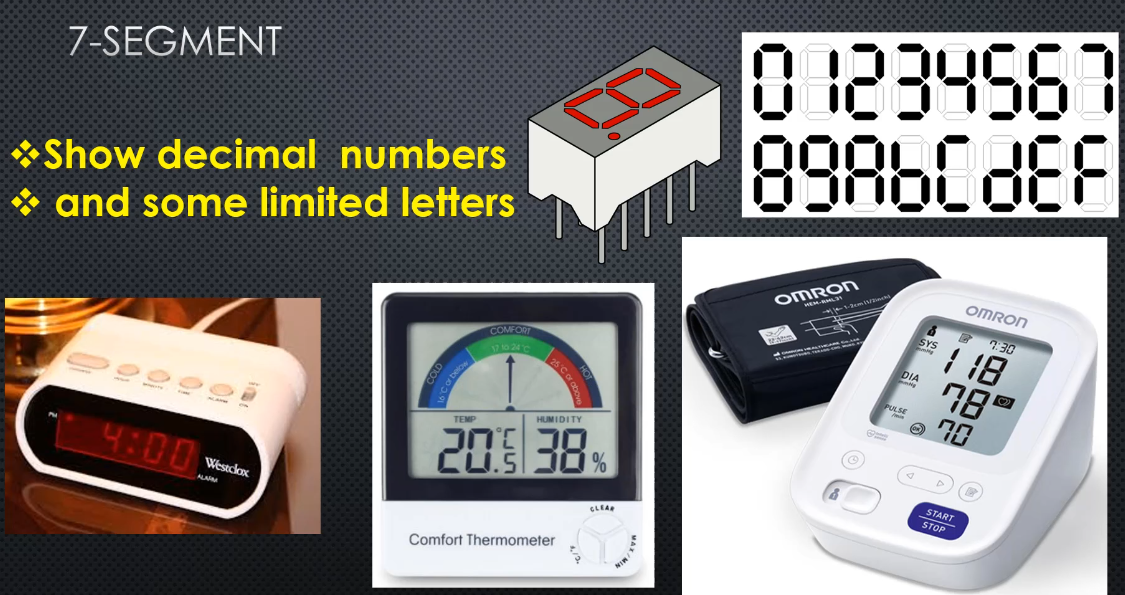
\includegraphics[scale=0.30,frame]{Figures/seven_seg/applications}
\caption{Seven segement presence in many electronic systems}
\label{fig:seven_seg:applications}
\end{figure}

In this chapter, we learn how to deal with these display using \verb|HLS|.\\

\newpage

\subsection{Driver}
\label{sub:Driver}

The driver for this type of display should contains 2 group of signals as shown in \autoref{fig:seven_seg:driver}:

\begin{itemize}

\item Data signal: control which number to be displayed

\item Control signal: select the target, that is which sgement we want to use.

\end{itemize}

\begin{figure}[h]
\centering
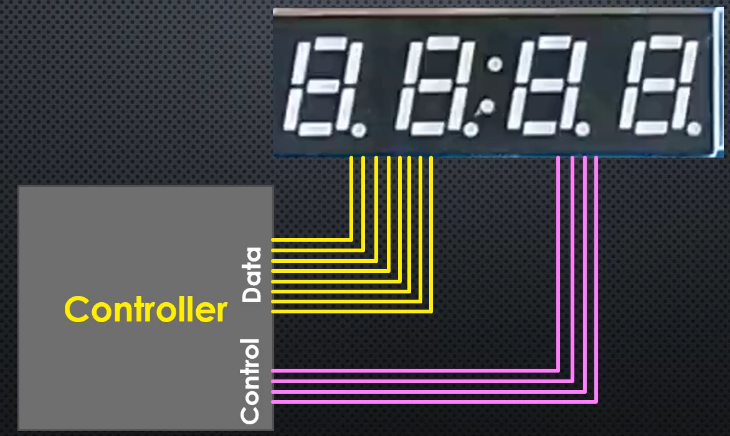
\includegraphics[scale=0.35,frame]{Figures/seven_seg/driver}
\caption{Signals for 7 segment}
\label{fig:seven_seg:driver}
\end{figure}


\underline{Notes regarding 7 Segement:}

\begin{itemize}

\item Multiple 7 segment share the same data signals and use them in a multiplex fashion managed by control signals.

\item The 7 segment uses a sequential circuit part, but in this chapter we focus on the combinational part, and explain some simple circuit and examples

\end{itemize}

\todo{7 Segment Notes:} \uti{7 Segment Notes:}

\begin{itemize}

\item \textit{To see what it does mean about the $\mathrm{1}^\mathrm{st}$ point above about sharing the same data signals} 

\item \textit{To be seen this later once I start reviewing the logic desing course and make the recap}

\end{itemize}

\newpage
\section{7 Segement Structure}
\label{sec:7seg_structure}

Now to dive into more technical details for 7 segment.\\

7 segment consist of 8 LED: 7 LED from A $\rightarrow$ G to display a digit, and 1 LED to display the digit point denoted as DP.

\begin{figure}[h]
\centering
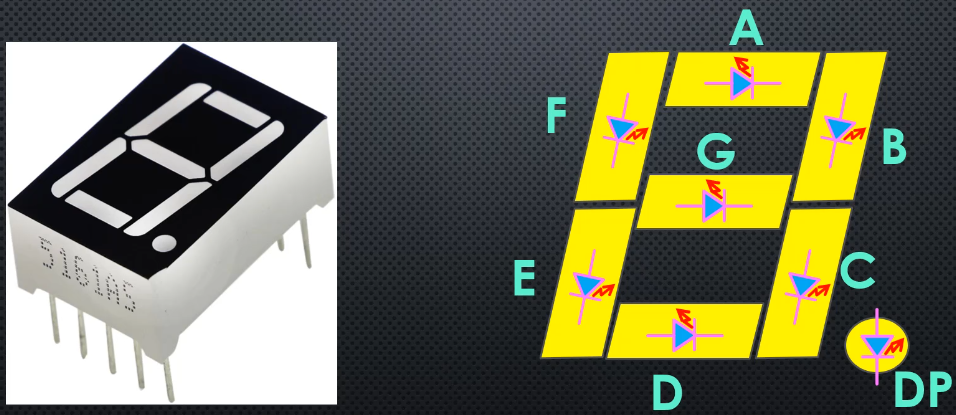
\includegraphics[scale=0.35,frame]{Figures/seven_seg/7seg_led}
\caption{7 segment LED structure}
\label{fig:seven_seg:7seg_led}
\end{figure}

7 segment has 2 types of connections: common anode and common cathode. In these configurations, multiple LED are connected together to a single point.


\begin{figure}[h]
\centering
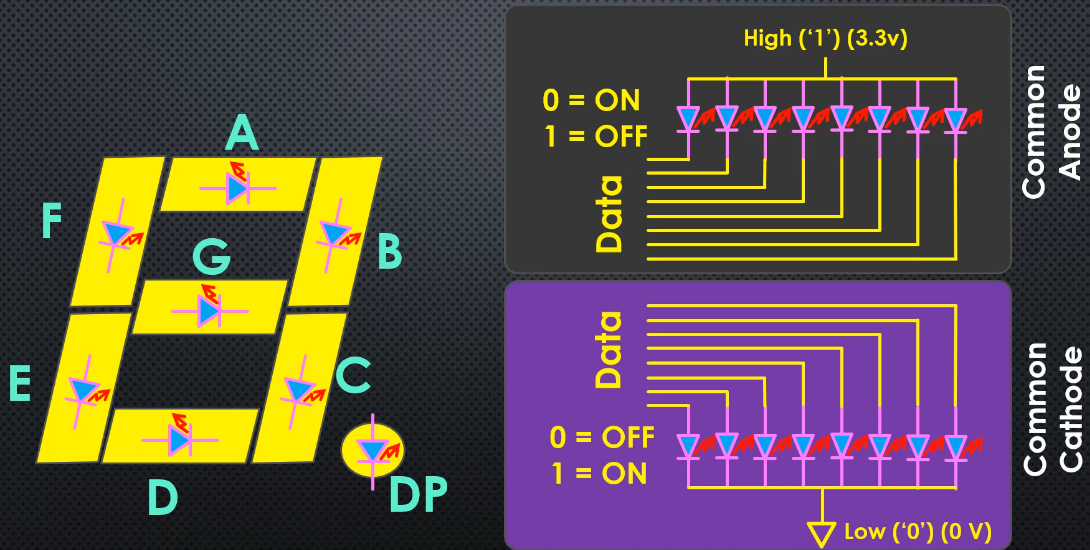
\includegraphics[scale=0.35,frame]{Figures/seven_seg/7seg_conf}
\caption{7 segment LED configuration: common anode and common cathode}
\label{fig:seven_seg:7seg_conf}
\end{figure}

\begin{itemize}

\item Common anode is where the $+$ side of the LED are connected to high voltage. In this configuration, a logic value of 0 turns the LED ON.

\item Common cathode is where the $-$ side are connected to low voltage. Therefore, a logic value of 1 turns a segment ON.

\end{itemize}


\newpage
\todo{Common Anode and cathode, insert in an appendix} \uti{Common Anode and cathode, insert in an appendix:}

\begin{itemize}

\item \textit{To make a review later about the circuit concept, like :}

	\begin{itemize}
	\item \textit{Common anode, cathode}
	
	\item \textit{Current flow,$\cdots$}
	\end{itemize}

\item \textit{To insert all these concepts in an appendix later}

\end{itemize}

To control a 7 segment regardless of the code which drives the 7 segment, a switch is used to turn ON or OFF the 7 segment. An example is shown in \autoref{fig:seven_seg:7seg_switch}.

\begin{figure}[h]
\centering
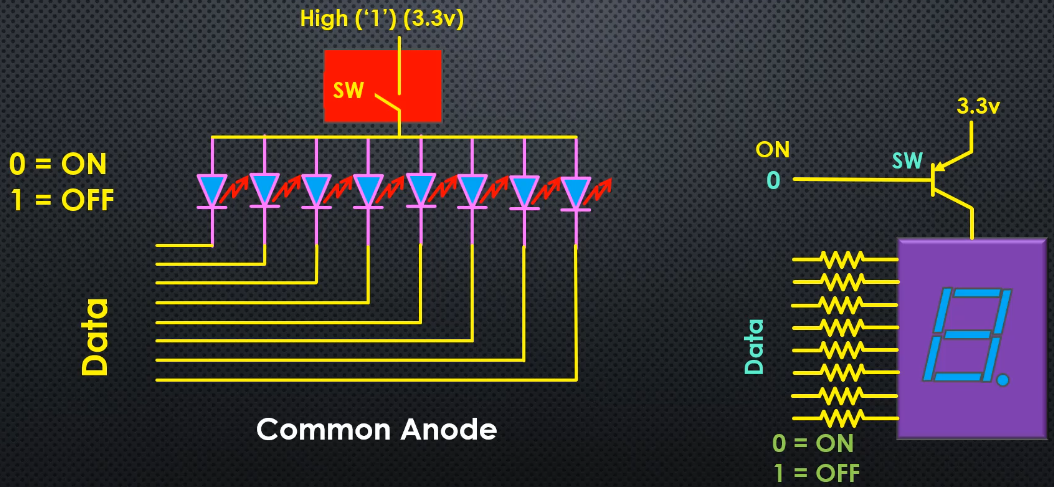
\includegraphics[scale=0.35,frame]{Figures/seven_seg/7seg_switch}
\caption{Switch control for a 7 segment using common anode configuration}
\label{fig:seven_seg:7seg_switch}
\end{figure}

\begin{itemize}

\item To turn ON the 7 segment, the switch should be driven by the logic value zero and

\item Proper data should be applied to the cathode

\end{itemize}

\newpage
\subsection{Quiz}

\underline{Quiz:} Find the logic values in the control and data signals to show the number 4 on this common anode 7 segment of \autoref{fig:seven_seg:quiz_7seg}.

\begin{figure}[h]
\centering
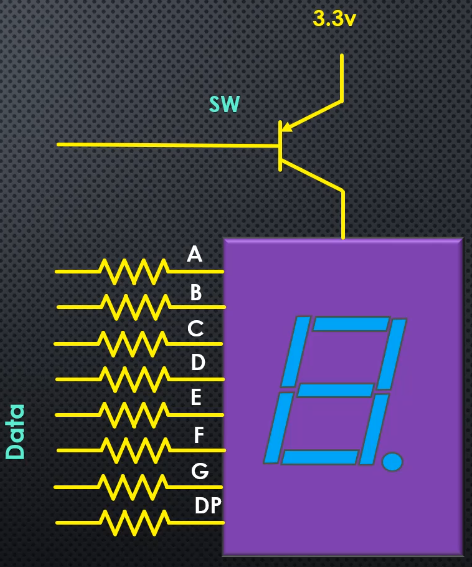
\includegraphics[scale=0.37,frame]{Figures/seven_seg/quiz_7seg}
\caption{Quiz 7 Segment}
\label{fig:seven_seg:quiz_7seg}
\end{figure}

\underline{Solution:}

\begin{itemize}

\item To turn on the 7-segment, the control signal connected to the PNP transistor switch should be 0.

\item To show the number 4, the data signal should turn on the LEDs on the four segments $B$, $C$, $F$ and $G$. So, as the 7-segment configuration is common anode the data is $0b10011001$

\end{itemize}

\begin{figure}[h]
\centering
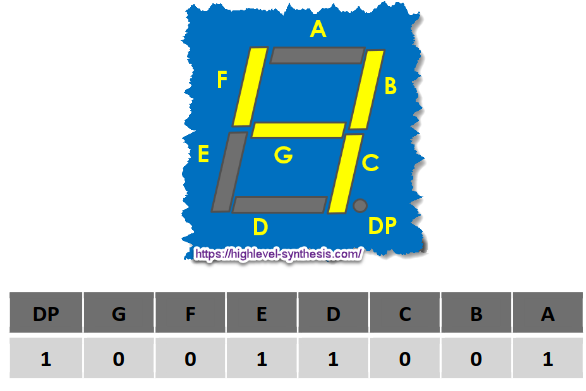
\includegraphics[scale=0.37,frame]{Figures/seven_seg/quiz_7seg_sol}
\caption{Quiz 7 Segment Solution}
\label{fig:seven_seg:quiz_7seg_sol}
\end{figure}

\newpage
\section{Digit Codes}
\label{sec:digit_codes}

\autoref{fig:seven_seg:anode_digit_codes} shows the different digit codes for common anaode configuration, where the control signal should be 0, and the data line also should be 0.

\begin{figure}[h]
\centering
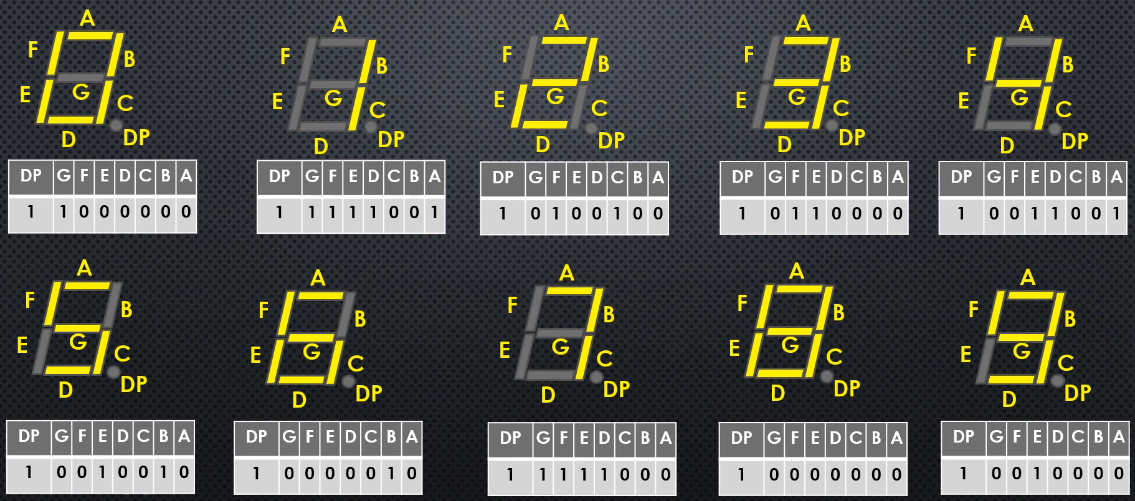
\includegraphics[scale=0.42,frame]{Figures/seven_seg/anode_digit_codes}
\caption{Digit codes for common anaode configuration}
\label{fig:seven_seg:anode_digit_codes}
\end{figure}

In a \verb|HLS| program, we can store these digit codes in an array and access them by their index as shown in \autoref{fig:seven_seg:codes_in_array}.


\begin{figure}[h]
\centering
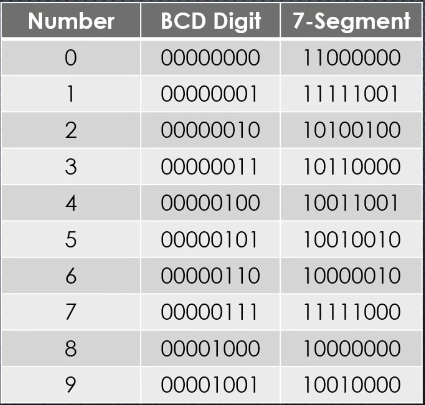
\includegraphics[scale=0.40,frame]{Figures/seven_seg/codes_in_array}
\caption{Digit codes stored in an array}
\label{fig:seven_seg:codes_in_array}
\end{figure}


\newpage
\section{7-Segment on Basys3}

After understanding general concepts of 7 segment circuit, we move to see the 7 segment on \verb|Basys3| board.\\


The \verb|Basys 3| board contains 4 segment display shown in \autoref{fig:seven_seg:basys3_7_seg}.

\begin{figure}[h]
\centering
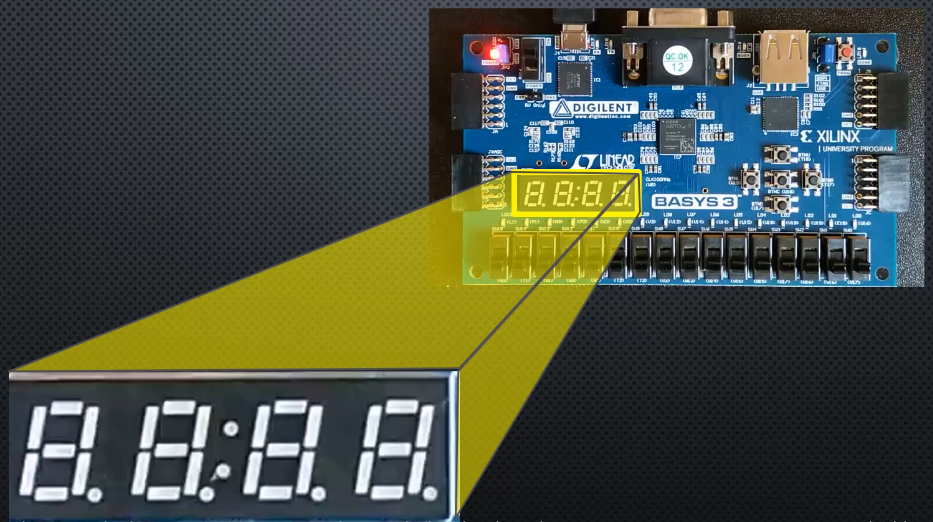
\includegraphics[scale=0.32,frame]{Figures/seven_seg/basys3_7_seg}
\caption{7 Segment on Basys 3}
\label{fig:seven_seg:basys3_7_seg}
\end{figure}

The pins configuration is shown in \autoref{fig:seven_seg:basys3_7seg_datasheet}.

\begin{figure}[h]
\centering
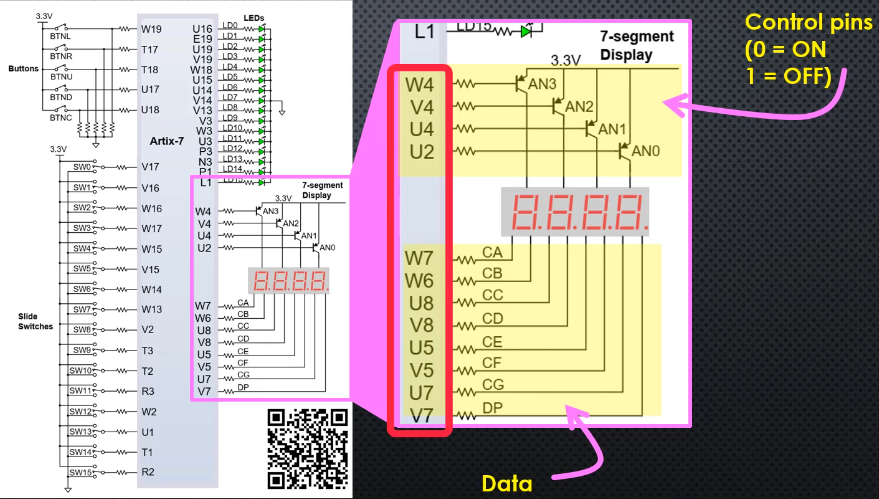
\includegraphics[scale=0.38,frame]{Figures/seven_seg/basys3_7seg_datasheet}
\caption{7 Segment pins configuration on Basys 3}
\label{fig:seven_seg:basys3_7seg_datasheet}
\end{figure}

\begin{itemize}

\item 12 pins are dedicated for the 4 7-seg:

	\begin{itemize}
	\item 4 pins for controls, where we have transistors acting a switch 
	
	\item 8 pins for data lines, shared among the 4 7-seg
	\end{itemize}

\item To display a digit using a 7-seg, and since the data lines are shared, \textit{time multiplexing} technique should be applied to the data signals

	\begin{itemize}
	\item Multiplexing requires a \textit{sequential desing}, which we will see in next chapters
	
	\item \todo{Multiplexing for 7 seg} \uti{Multiplexing for 7 seg:} \textit{To review this topic when started later in the sequential desing course}
	
	\item \textit{To cite the chapter later here}
	 
	\end{itemize}	   

\end{itemize}


\subsection{Quiz}

\underline{Quiz:} Find the control signal value and data code to write the number 5 on the left hand side 7 segment (according to \autoref{fig:seven_seg:basys3_7seg_datasheet}) and turn off the others.\\

\underline{Solution:}

\begin{itemize}

\item To enable the left-hand side display, we should apply 0 on W4 pin

\item To disable the others, V4, U4 and U2 should receive the logic value 1.

\item The code on the data pins is 0b10010010

\end{itemize}


\begin{figure}[h]
\centering
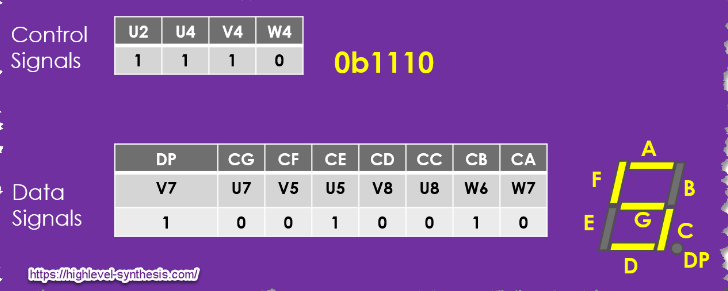
\includegraphics[scale=0.42,frame]{Figures/seven_seg/quiz_7seg_basys3_sol}
\caption{7 Segment quiz solution}
\label{fig:seven_seg:quiz_7seg_basys3_sol}
\end{figure}


\newpage
\section{1 Digit Example}

Now we take an example about 7 segment, and try implement it using \verb|HLS|. The given is shown in \autoref{fig:seven_seg:1digit_example}.

\begin{figure}[h]
\centering
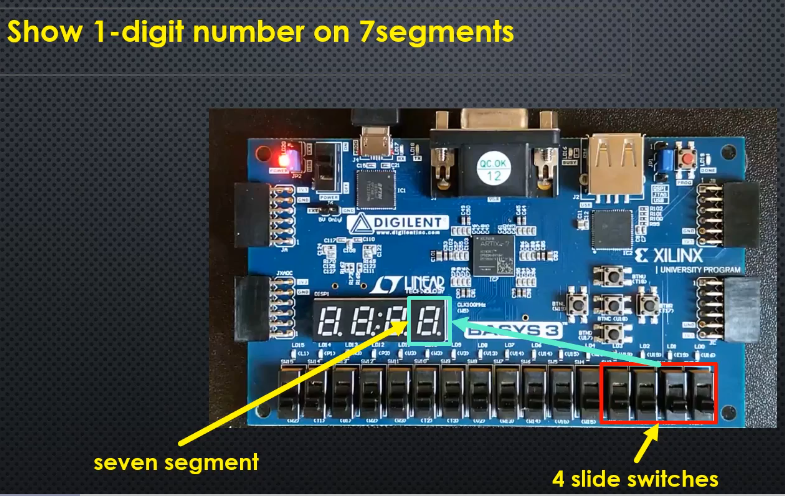
\includegraphics[scale=0.35,frame]{Figures/seven_seg/1digit_example}
\caption{Given of 1 digit example using 7 segment}
\label{fig:seven_seg:1digit_example}
\end{figure}

\subsection{Algorithm}

The algorithm that controls the 7 segment has 3 steps:

\begin{enumerate}

\item Get the digit binary code

\item Encoding the binary code into 7 segment code

\item Drive the target 7 segment display in the code

\end{enumerate}

These steps are illustrated in \autoref{fig:seven_seg:1digit_algo_step}.

\begin{figure}[h]
\centering
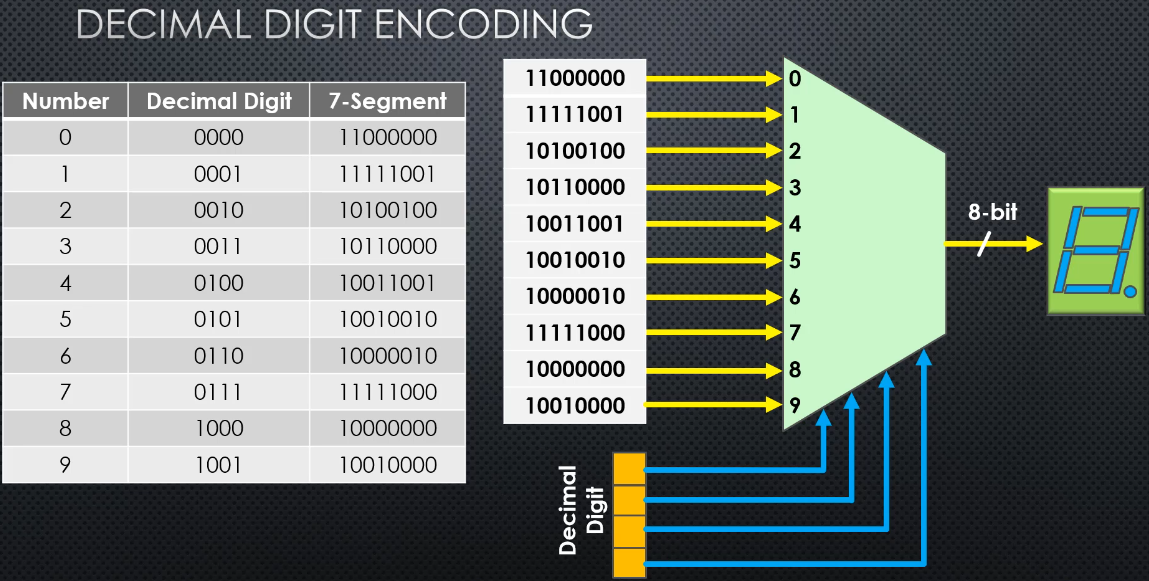
\includegraphics[scale=0.35,frame]{Figures/seven_seg/1digit_algo_step}
\caption{Steps of 1 digit algorithm display}
\label{fig:seven_seg:1digit_algo_step}
\end{figure}

\begin{itemize}

\item We have at the left side a table mapping the binary code of a digit to its corresponding 7 segment code

\item A MUX is used to encode binary representation of a digit into 7 segment code

	\begin{itemize}
	\item The binary code act as control signals for the MUX
	
	\item The 7 segment codes are input for the MUX
	\end{itemize}

\end{itemize}

\subsection{HLS Code}

The \verb|HLS| code is shown in \autoref{fig:seven_seg:1digit_hls}.

\begin{figure}[h]
\centering
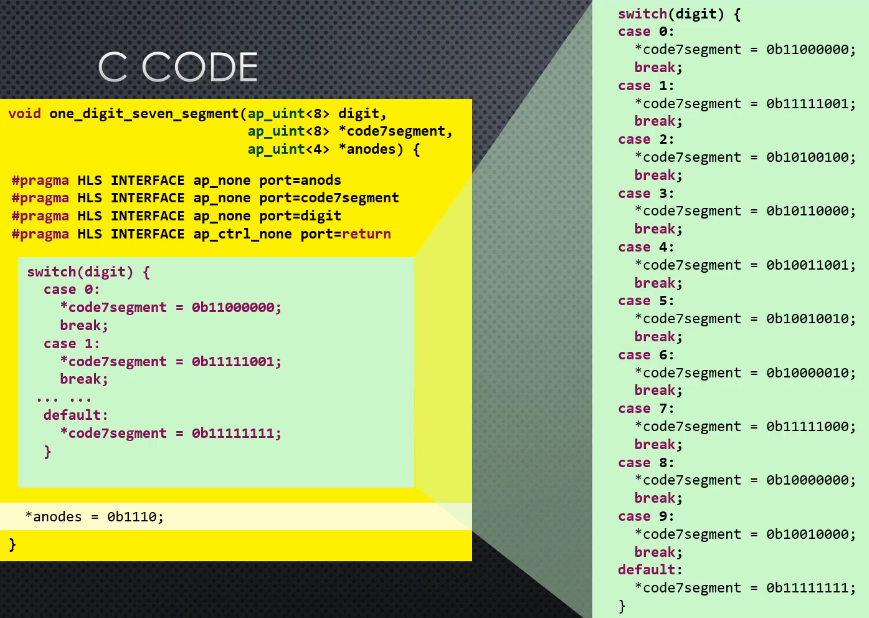
\includegraphics[scale=0.40,frame]{Figures/seven_seg/1digit_hls}
\caption{HLS code for 1 digit display}
\label{fig:seven_seg:1digit_hls}
\end{figure}

\newpage
\section{BCD Code}
\label{sec:BCD_code}

It is true that underlying computation in logic uses binary, but decimal number are more intuitive, this why BCD codes were invented, to make a transformation from binary to decimal, and display them in the 7 -seg.

The goal in this section is to see how to move from binary representation to BCD code, then display it on 7-seg.\\

Recall that a BCD for a number is \textit{the concatenation of its binary representation of its digit} . An example is shown in \autoref{fig:seven_seg:bcd_intro}, where we have the BCD of 24.

\begin{figure}[h]
\centering
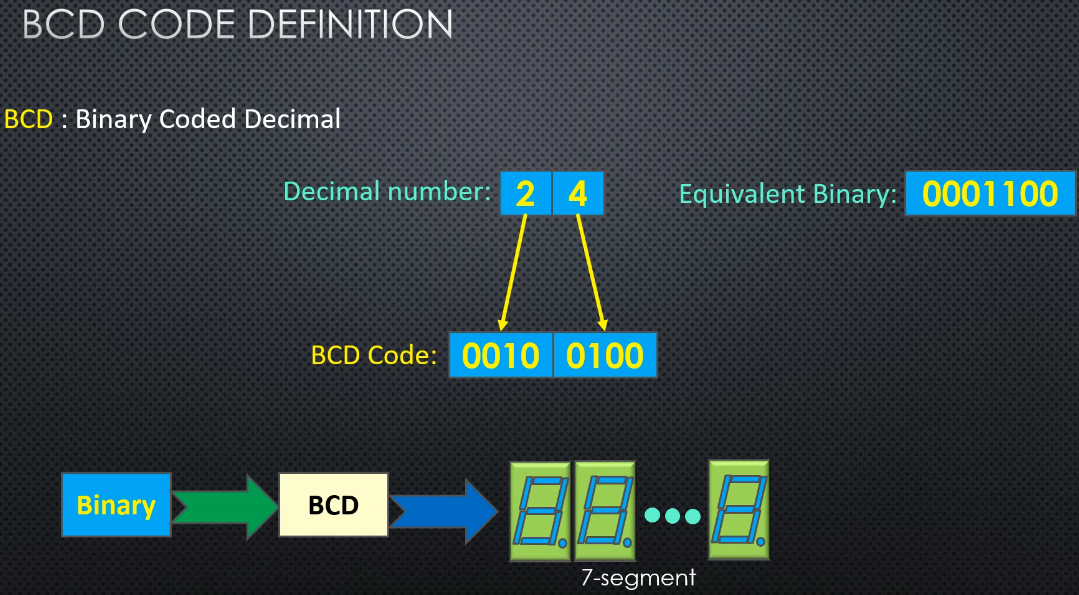
\includegraphics[scale=0.38,frame]{Figures/seven_seg/bcd_intro}
\caption{BCD definition}
\label{fig:seven_seg:bcd_intro}
\end{figure}

\newpage
\subsection{BCD Types and Memroy}

A 4 bit BCD can represent a decimal digit, but its saving in memory comes in different 2 different ways: packed and unpacaked. 

An example is shown in \autoref{fig:seven_seg:bcd_types}.

\begin{figure}[h]
\centering
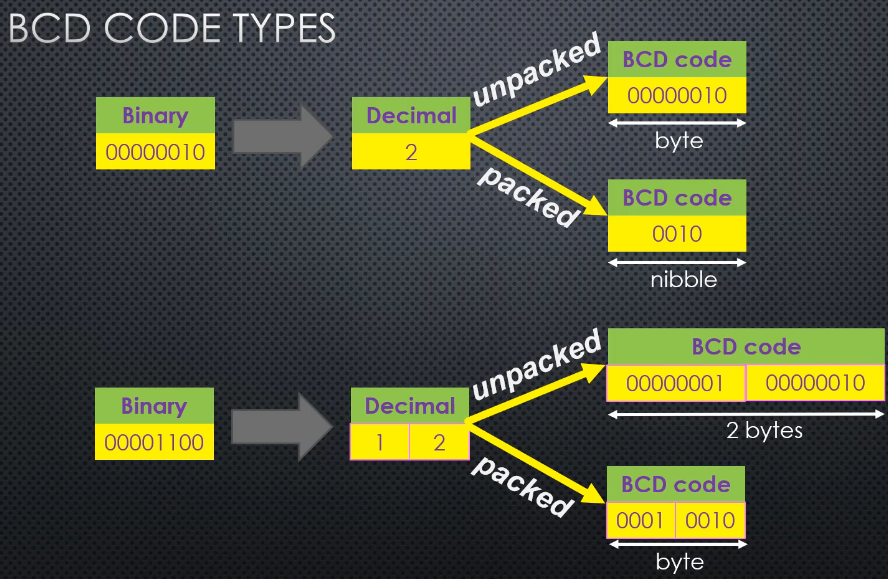
\includegraphics[scale=0.40,frame]{Figures/seven_seg/bcd_types}
\caption{BCD types}
\label{fig:seven_seg:bcd_types}
\end{figure}

\begin{itemize}

\item For the $\mathrm{1}^\mathrm{st}$ example, decimal 2:

	\begin{itemize}
	\item Unpacked version requires 8 bit, the upper 4 bit are all 0
		
	\item Packed version uses only 4 bit	
	\end{itemize}


\item For the $\mathrm{2}^\mathrm{nd}$ example, 12:

	\begin{itemize}
	\item Unpcaked requires 2 bytes of memory, since each digit require 8 bit (1 byte)
	\end{itemize}

\end{itemize}

\newpage
\subsection{Quiz}
\label{sub:binary_to_bcd}

\underline{Quiz:} Find the BCD code of the following binary number: 0b0001010001110100.\\


\underline{Solution:}\\

The decimal value of 0b0001010001110100 is 5 236. We take then the binary representation of each digit, and the BCD code will be the concatenation of each compact BCD digit as shown in \autoref{fig:seven_seg:qui_bcd_sol}.

\begin{figure}[h]
\centering
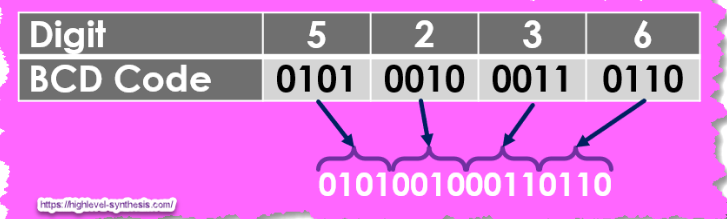
\includegraphics[scale=0.38,frame]{Figures/seven_seg/qui_bcd_sol}
\caption{BCD quiz solution}
\label{fig:seven_seg:qui_bcd_sol}
\end{figure}

\newpage
\section{HLS: Binary to BCD}
\label{sec:hls_binary_to_bcd}

Now our goal is to desing some combinational circuit using \verb|HLS| the convert some binary representation to BCD representation.\\

We study 3 methods to do such a conversion:

\begin{enumerate}

\item Modulo algorithm

\item A modified version of 1, withou a \verb|while| loop

\item The double dabble method, which uses shift operations and add 3

\end{enumerate}

\subsection{Modulo Method}

\autoref{fig:seven_seg:binary_to_bcd_hls} shows the algorithm along with some example in the right hand side

\begin{figure}[h]
\centering
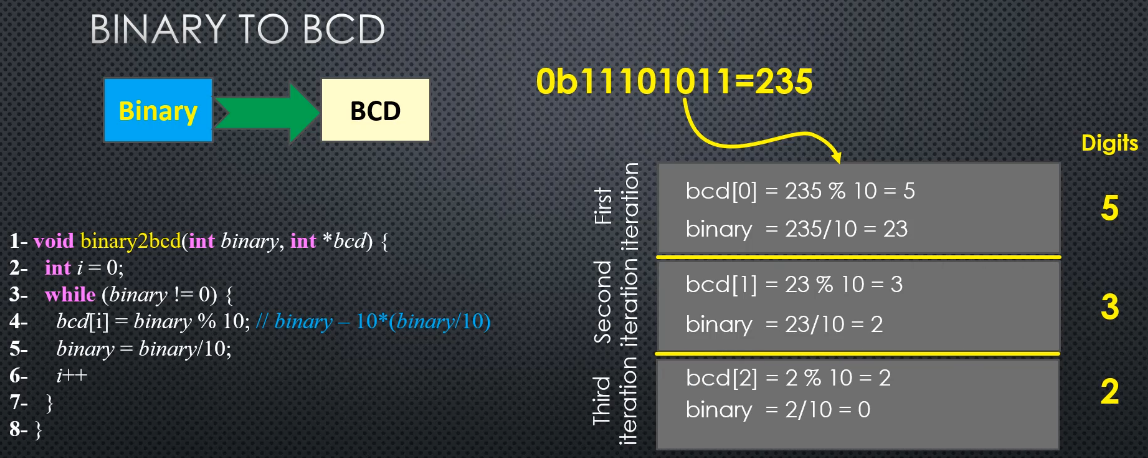
\includegraphics[scale=0.40,frame]{Figures/seven_seg/binary_to_bcd_hls}
\caption{Binary to BCD program}
\label{fig:seven_seg:binary_to_bcd_hls}
\end{figure}


\begin{itemize}

\item The input \verb|int binary| is 235

\item In the $\mathrm{1}^\mathrm{st}$ iteration, the algorithm extract the LSB digit from 235 using the \verb|%| operator

	\begin{itemize}
	\item Then it modifies the \verb|binary| by dividing by 10, so we can extract it the next digit in the next iteration
	\end{itemize}

\end{itemize}

The \verb|while| loop implies the usage of some sequential circuit, so we try to get rid of it (for now) and see how can we use some other approach.

\newpage
\subsection{Modified Algorithm}

Since we are working on \verb|Basys3| board which uses 4 7-segment, we assume that the number to be represented is in a range from $0 \, \rightarrow \, 9999$. \\

Also the \verb|while| loop of \autoref{fig:seven_seg:binary_to_bcd_hls} contains 2 arithmetic computation step, we will encapsulate these steps into some function and call this function 4 times (equal to 4 7-seg in \verb|Basys3|) board.

These modifications are shown in \autoref{fig:seven_seg:binary_to_bcd_modified}.

\begin{figure}[h]
\centering
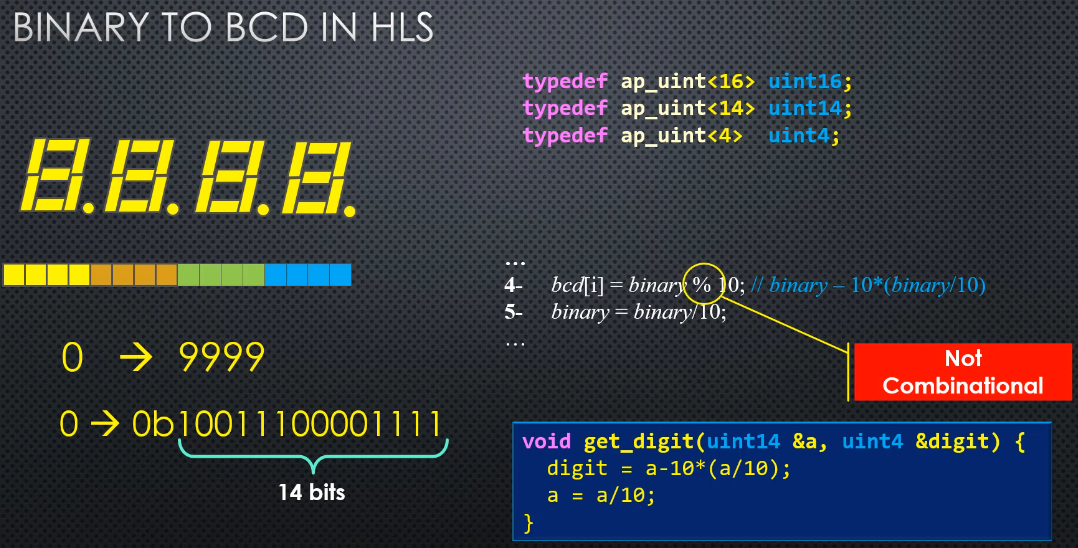
\includegraphics[scale=0.40,frame]{Figures/seven_seg/binary_to_bcd_modified}
\caption{Binary to BCD program modifications}
\label{fig:seven_seg:binary_to_bcd_modified}
\end{figure}

\begin{itemize}

\item For the data type

	\begin{itemize}
	\item for the input binary we need 14 bit number

	\item 4 bits to represent BCD code for a single digit			
 
	\item 16 bits to send out the BCD code to the 4 7-seg
	
	\end{itemize}

\item The \verb|%| operator is not in general a combinational circuit, so we use the equivalent statment \verb|a-10*(a/10)|

\end{itemize}

\newpage
The final code in \verb|HLS| using the modifications discusses above is shown in \autoref{fig:seven_seg:binary_to_bcd_modified_hls}.

\begin{figure}[h]
\centering
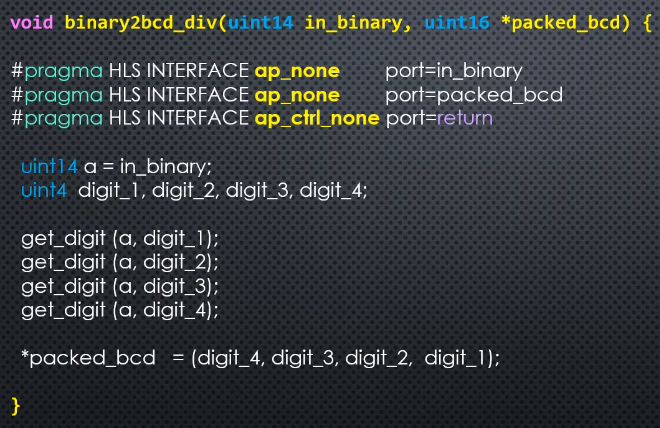
\includegraphics[scale=0.40,frame]{Figures/seven_seg/binary_to_bcd_modified_hls}
\caption{Binary to BCD program HLS code with modifications}
\label{fig:seven_seg:binary_to_bcd_modified_hls}
\end{figure}

\subsection{Double Dabble Algorithm}
\label{sub:double_dabble}

Now we explain a more efficient algorithm named \textit{double dabble}. This algorithm uses 2 operators: shift left and add 3.\\

\underline{Points of the algorithm:}

\begin{itemize}

\item We need a variable to store both binary and BCD numbers

	\begin{itemize}
	\item The variable should have enough space for both numbers
	\end{itemize}

\item 	The binary number is saved on the righ hand side of the variable, and BCD number (packed version) is hosted on the left side, and initialized to 0

	\begin{itemize}
	\item Recall for BCD number, we use 4 bits for each digit in packed version
	\end{itemize}

\item  For an $n$ bit binary number, the double dabble algorithm is perfomed $\left(\, n \, - \, 1 \, \right)$

\end{itemize}

\newpage
The steps of the algorithm in addition to a runnning example is shown in \autoref{fig:seven_seg:double_dabble_algo}.

\begin{figure}[h]
\centering
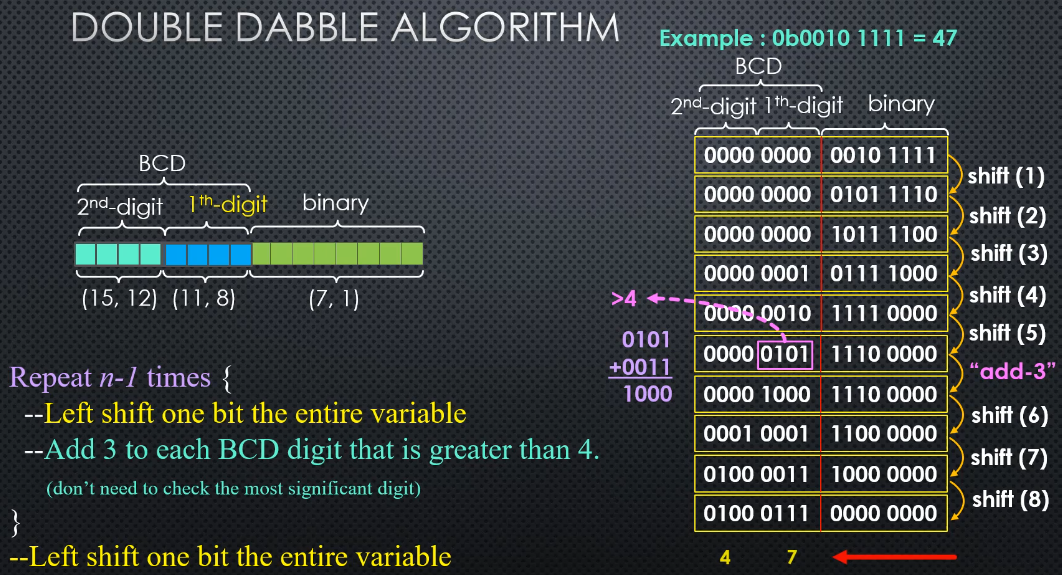
\includegraphics[scale=0.40,frame]{Figures/seven_seg/double_dabble_algo}
\caption{Binary to BCD using double dablle algorithm}
\label{fig:seven_seg:double_dabble_algo}
\end{figure}

\begin{itemize}

\item The input of the algorithm is 8 bit binary number, and 8 bit for the BCD code for 2 digit (4 bit for each digit)

\item After the $\mathrm{5}^\mathrm{th}$ shift, the $\mathrm{1}^\mathrm{st}$ BCD digit has a value of 5 ($> 4$). So we add 3 to it

\item Then we continue shifting to the left the rest of the binary variable

\end{itemize}

The \verb|HLS| code is shown in \autoref{fig:seven_seg:double_dabble_hls}.

\begin{figure}[h]
\centering
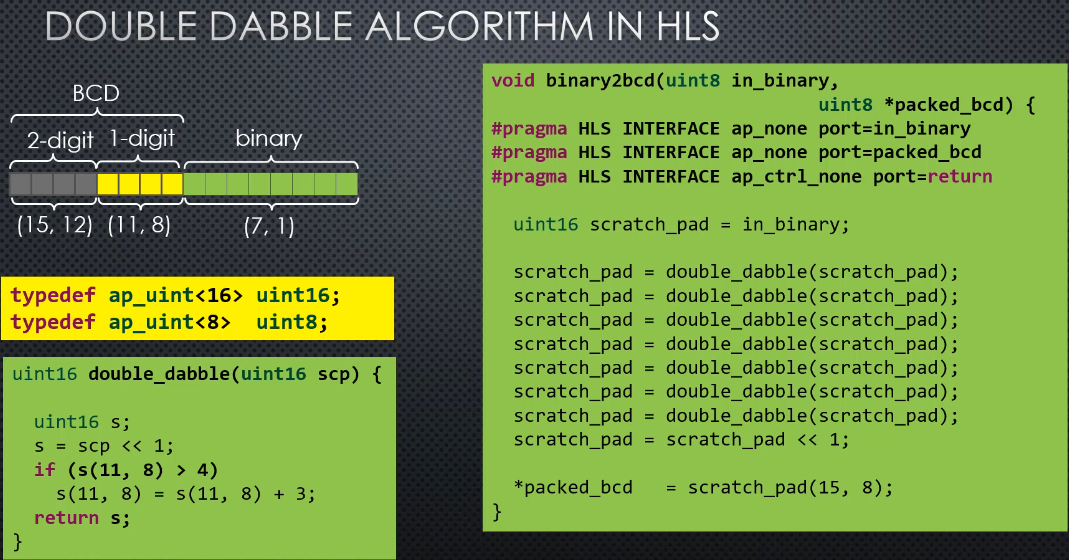
\includegraphics[scale=0.40,frame]{Figures/seven_seg/double_dabble_hls}
\caption{Double dablle algorithm in HLS}
\label{fig:seven_seg:double_dabble_hls}
\end{figure}


\newpage
\section{2 Digit Code}

Afer seeing the algorithm that turns a binary number to a BCD code, we move to the implementation on \verb|Basys3| board, and try to display 2 digit code.\\

Tha approach is shown in \autoref{fig:seven_seg:bcd_2_digit}.

\begin{figure}[h]
\centering
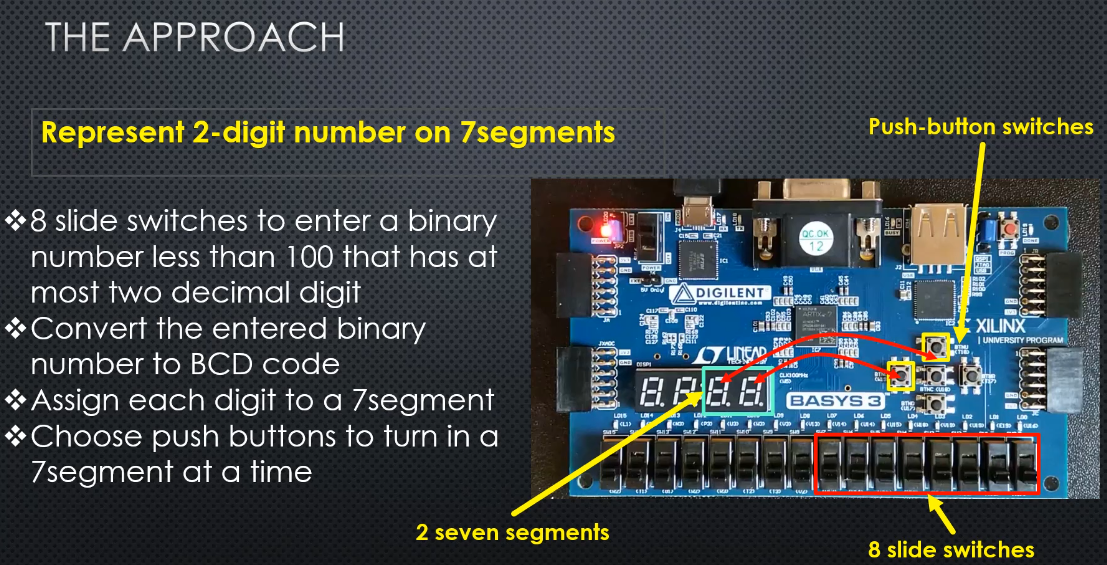
\includegraphics[scale=0.40,frame]{Figures/seven_seg/bcd_2_digit}
\caption{BCD for 2 digit on Basys3 FPGA}
\label{fig:seven_seg:bcd_2_digit}
\end{figure}

The steps and the \verb|HLS| code is shown in \autoref{fig:seven_seg:bcd_2_digit_steps_hls}.

\begin{figure}[h]
\centering
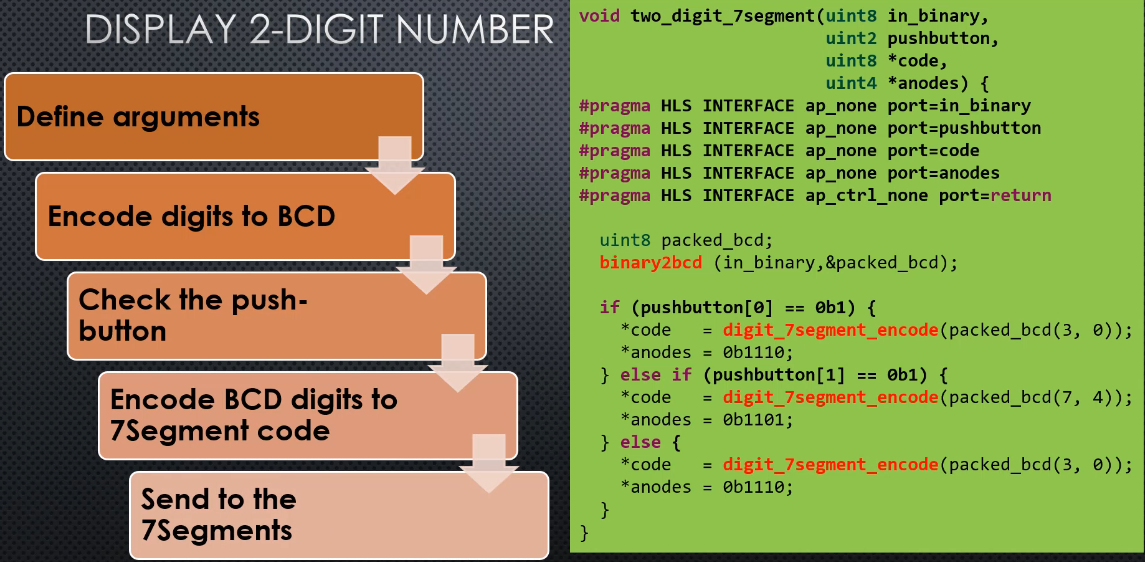
\includegraphics[scale=0.40,frame]{Figures/seven_seg/bcd_2_digit_steps_hls}
\caption{BCD for 2 digit steps and HLS code}
\label{fig:seven_seg:bcd_2_digit_steps_hls}
\end{figure}

\newpage
\subsection{Quiz}

\underline{Quiz:} Write an \verb|HLS| code to show a 4 digit number on 7-segments. Use push button as shown in \autoref{fig:seven_seg:quiz_4_digit} to activate each 7 segment.

\begin{figure}[h]
\centering
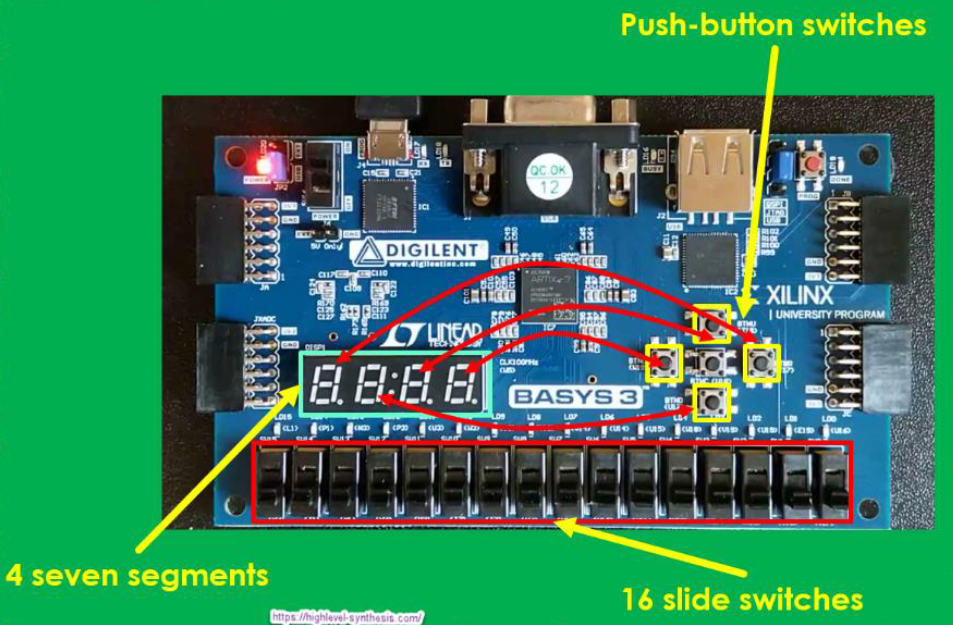
\includegraphics[scale=0.33,frame]{Figures/seven_seg/quiz_4_digit}
\caption{Push buttons mapping to active 7 segment}
\label{fig:seven_seg:quiz_4_digit}
\end{figure}

\underline{Solution:} The \verb|HLS| code is shown in \autoref{fig:seven_seg:quiz_4_digit_sol}.

\begin{figure}[h]
\centering
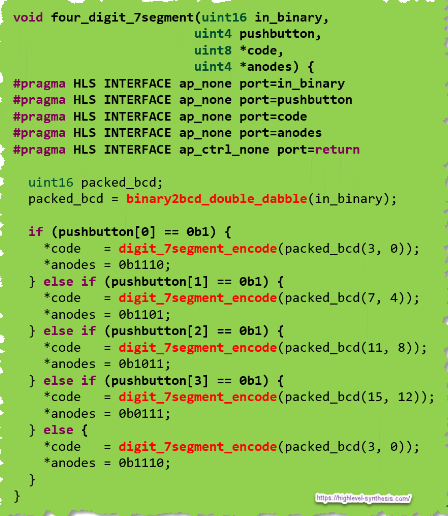
\includegraphics[scale=0.48,frame]{Figures/seven_seg/quiz_4_digit_sol}
\caption{Push buttons mapping to active 7 segment}
\label{fig:seven_seg:quiz_4_digit_sol}
\end{figure}


\newpage
\section{Exercices}

\todo{7Seg Ex} \uti{7Seg Ex:}

\begin{itemize}

\item \textit{To do these exercices later}

\item \textit{Insert comment and solution in readme file or the report}

\end{itemize}

\begin{enumerate}

\item Design a logic circuit that receives a four-digit compact BCD code and returns its equivalent binary value.

\item Show a four-digit hex number on the 7-segments available on the Basys3 board. Use the slide switches to enter the number. In addition, use the pushbuttons as shown in \autoref{fig:seven_seg:ex_2_7seg} to activate a 7-segment at a time.

\begin{figure}[h]
\centering
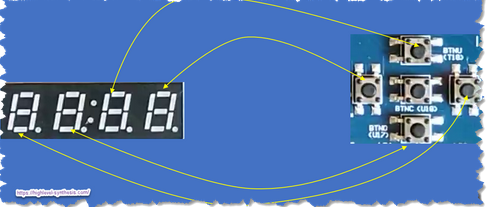
\includegraphics[scale=0.48,frame]{Figures/seven_seg/ex_2_7seg}
\caption{Exercie 2 given}
\label{fig:seven_seg:ex_2_7seg}
\end{figure}

\item Design a logic circuit that gets the ASCII codes corresponding to the lower-case letters a, b, c, d, e, f, g, h, l and show them on a right-hand side 7-segment. Use the slide switches to enter an ASCII code. \autoref{fig:seven_seg:ex_3_table} shows the ASCII codes for these letters.

\begin{figure}[h]
\centering
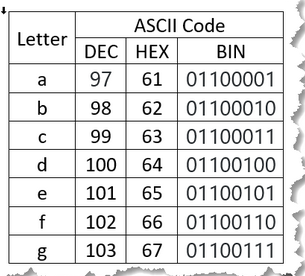
\includegraphics[scale=0.48,frame]{Figures/seven_seg/ex_3_table}
\caption{Exercie 3 ASCII table}
\label{fig:seven_seg:ex_3_table}
\end{figure}


\end{enumerate}



\newpage
\section{Summary}

\begin{itemize}

\item Signals for 7-Seg (\ref{sub:Driver})

	\begin{enumerate}
	\item Control signal $\leftrightarrow$ segment selection 
	
	\item Data signal $\leftrightarrow$ digit value
	\end{enumerate}

\item Configuration (\ref{sec:7seg_structure}):

	\begin{itemize}
	\item Common anode: $+$ side of LED to high voltage, and logic 0 turn LED ON
	
	\item Common cathode: $-$ side of LED to ground, and logic 1 to turn LED ON
	
	\item \autoref{tab:7seg_conf} group these configuration
	
	\begin{table}[h!]
\centering

\begin{tabular}{|c|c|c|}
\hline
Configuration & Common Anode & Common Cathode \\
\hline
Shared terminal & All anodes to Vcc & All cathodes tied to GND \\ \hline
\multirow{2}{*}{Segment control} & Each segment has its own cathode  & Each segment has its own anode  \\ \cline{2-3}
& separate cathode & separate anode \\ \hline
Turn ON segment (LED) & Logic 0 & Logic 1  \\ \hline
FPGA boards & Basys3 & \\ \hline
\end{tabular}
\caption{Comparison of Common Anode vs Common Cathode LED configurations}
\label{tab:7seg_conf}
\end{table}
	
	 
	\end{itemize}

\item BCD codes (\ref{sec:BCD_code})

	\begin{itemize}
	\item Single digit (as in 4): same as binary representation 
	
	\item multiple digit (as 47): concatenation of binary code for each digit
	
	\item From binary to BCD (\ref{sub:binary_to_bcd}):
	
		\begin{enumerate}
		\item get back to decimal
		
		\item Take each digit in binary representation form
		
		\item Concatenate the result
		\end{enumerate}
	
	
	\end{itemize}

\item Binary to BCD (\ref{sec:hls_binary_to_bcd}): 

This section contains method to transform a binary number into its BCD code. 


\item  We recap the double dabble algorithm (\ref{sub:double_dabble}):

Take as example an $n \, = \, 8 $ bit binary \verb|0b0010 1111| ($= 47$).

For $ n -1$ times (that is 7 in our case): 

\begin{itemize}

\item we shift by 1 the binary number

\item We check if the BCD part if greater than 4, we add 3

\end{itemize}

After finishing the $n \, - \, 1$ iterations, we shift by 1 one last time for the MSB part.

\end{itemize}

\newpage
A summary about the steps learned in 7-seg is shown in \autoref{fig:seven_seg:summary_7seg}.

\begin{figure}[h]
\centering
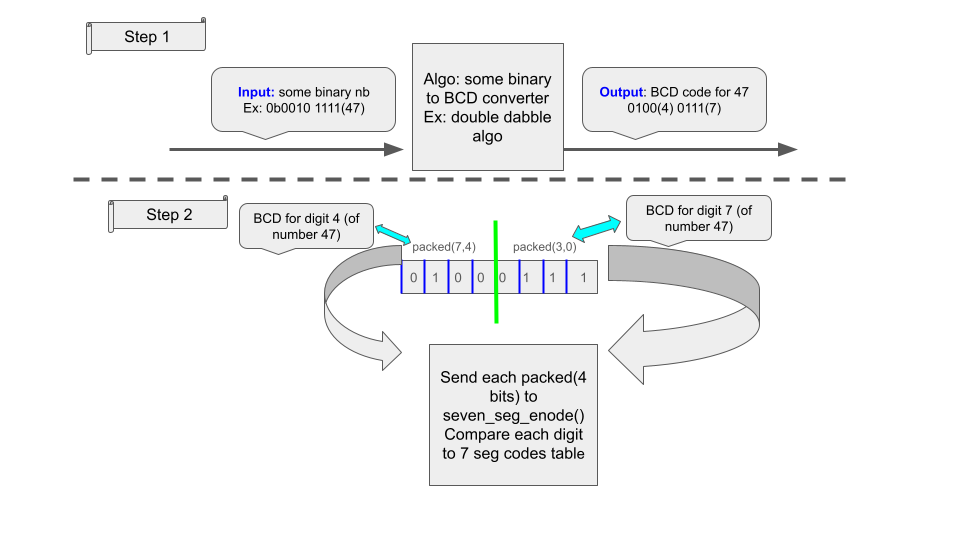
\includegraphics[scale=0.52,frame]{Figures/seven_seg/summary_7seg}
\caption{Summary for 7 Seg}
\label{fig:seven_seg:summary_7seg}
\end{figure}


\chapter{Combinational Loops}

\section{Introduction}

In this chapter we deal with \textit{loop} concept from hardware perspective, and see how to implement it using \verb|HLS|.\\

\todo{Intro combinational loop} \uti{Intro combinational loop:}

\begin{itemize}

\item \textit{To rewrite it later after finishing the chapter}

\end{itemize}

\newpage
\section{Definition}

$\mathrm{1}^\mathrm{st}$ let's take an example of \verb|for| loop statement, and see the scenrios in a software perspective, then move to hardware perspective. The example of software perspective is shown in \autoref{fig:comb_loop:loop_soft}.


\begin{figure}[h]
\centering
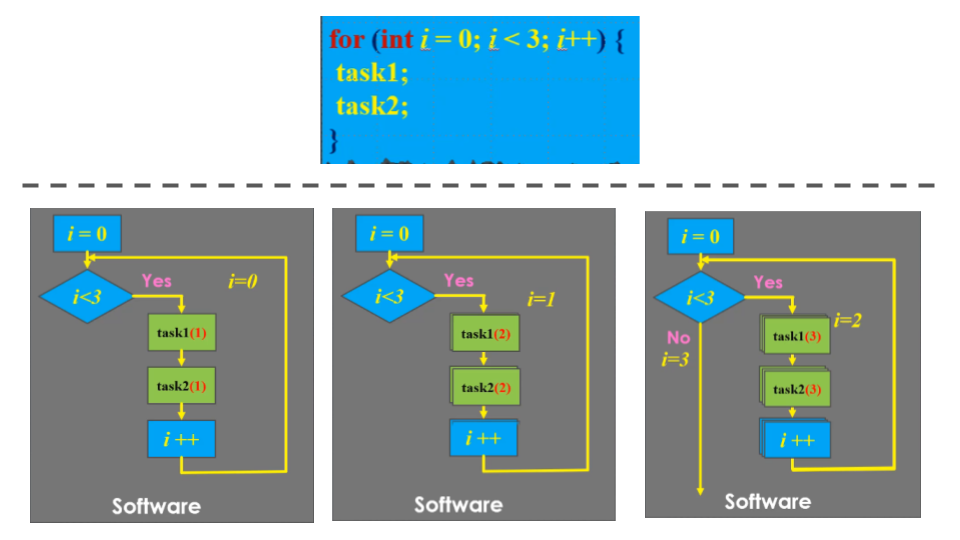
\includegraphics[scale=0.40,frame]{Figures/comb_loop/loop_soft}
\caption{For loop in a software execution}
\label{fig:comb_loop:loop_soft}
\end{figure}

\begin{itemize}

\item Notice that in each iteration, each \verb|task1| \verb|task2| has 1 instance invoked

	\begin{itemize}
	\item In other words, have 1 instance of \verb|taks1| and \verb|task2| used in all executions (iterations)
	\end{itemize}

\end{itemize}

Now unlike software concept, in hardware we have different instances (more like circuit modules) for each task in each iteration. In the \verb|for| loop example of \autoref{fig:comb_loop:loop_soft}, we have 3 iterations and 2 \verb|taskx| (\verb|1| and \verb|2|), so we obtain 6 instnaces in total, 3 for each \verb|task|.

Now concerning the flow of the loop, it is related to the  \tbi{dependency among data and iterations} between the tasks. 

\newpage
All different cases are shown in  \autoref{fig:comb_loop:loop_hardware}.

\begin{figure}[h]
\centering
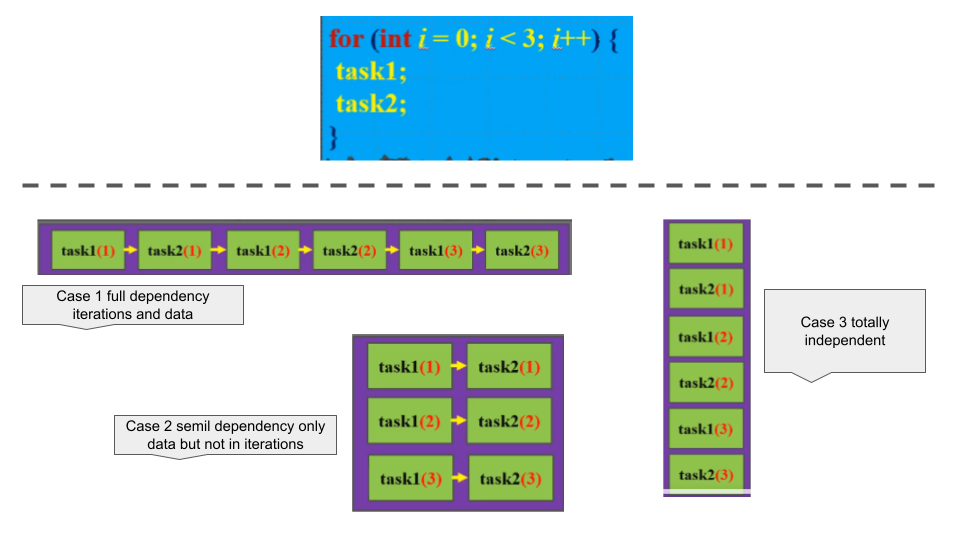
\includegraphics[scale=0.45,frame]{Figures/comb_loop/loop_hardware}
\caption{For loop in a hardware execution}
\label{fig:comb_loop:loop_hardware}
\end{figure}

\begin{itemize}

\item In case 1, because of full depdency, \verb|task2| need to wait for \verb|task1| (the data part), and in the next iterations also we need results, so \verb|task1(2)| need for both \verb|task1(1)| and \verb|task2(1)| to finish

	\begin{itemize}
	\item Full dependcy result in a sequential execution of the \verb|for| loop
	\end{itemize}

\item Case2 we only have dependncy among data, but not in iterations. This means \verb|task1(x)| in all iterations can run in parallel

\item Case 3 all the modules or instances are independent, hence all modules run in parallel.

\end{itemize}

\newpage
\subsection{Quiz}

\underline{Quiz 1:} Draw an execution graph for a  combinantional circuit that perform the \verb|for| loop shown in 
\autoref{fig:comb_loop:quiz_1_loop}.

\begin{figure}[h]
\centering
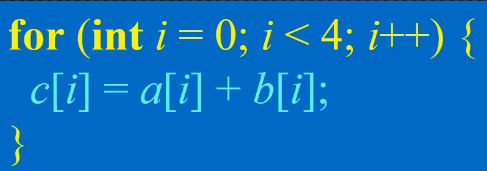
\includegraphics[scale=0.45,frame]{Figures/comb_loop/quiz_1_loop}
\caption{Quiz 1 for loop}
\label{fig:comb_loop:quiz_1_loop}
\end{figure}

\underline{Solution Quiz 1:} 
The data dependency plays a crucial role in the combinational circuit execution model. For this purpose, a graph can show the dependency relation between expressions. According to the \verb|for| loop body, the loop has three iterations that
are independent if arrays \verb|a|,\verb|b| and \verb|c| are stored in different memory areas.


Each iteration can be shown by a single graph node as shown in \autoref{fig:comb_loop:quiz_1_loop_graph}.


\begin{figure}[h]
\centering
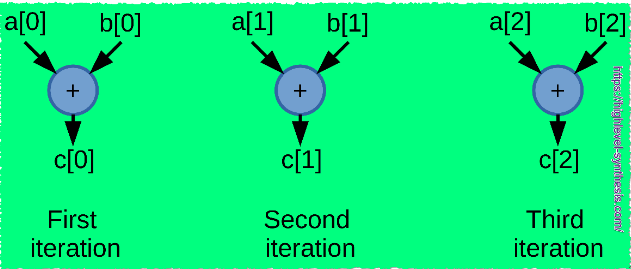
\includegraphics[scale=0.45,frame]{Figures/comb_loop/quiz_1_loop_graph}
\caption{Quiz 1 for loop graph}
\label{fig:comb_loop:quiz_1_loop_graph}
\end{figure}

As these iterations are independent, all of them can be executed in parallel that can be shown \autoref{fig:comb_loop:quiz_1_loop_execution}.

\begin{figure}[h]
\centering
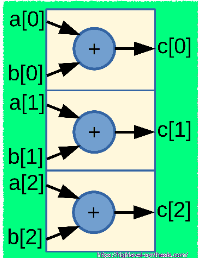
\includegraphics[scale=0.45,frame]{Figures/comb_loop/quiz_1_loop_execution}
\caption{Quiz 1 for loop execution}
\label{fig:comb_loop:quiz_1_loop_execution}
\end{figure}

\newpage
\underline{Quiz 2:} same as quiz 1, but the \verb|for| loop shown in \autoref{fig:comb_loop:quiz_2_loop}.

\begin{figure}[h]
\centering
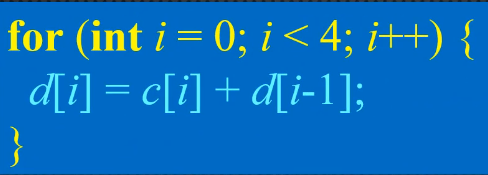
\includegraphics[scale=0.45,frame]{Figures/comb_loop/quiz_2_loop}
\caption{Quiz 2 for loop}
\label{fig:comb_loop:quiz_2_loop}
\end{figure}

\underline{Solution Quiz 2:}  As can be seen, each iteration of this for loop uses a data (denoted by $d[i-1]$) generated by its predecessor. Therefore, \tbi{there is a data dependency between two consecutive loop iterations in this code}.
Each addition in iteration can be seen by a graph node as shown in \autoref{fig:comb_loop:quiz_2_loop_graph}.

\begin{figure}[h]
\centering
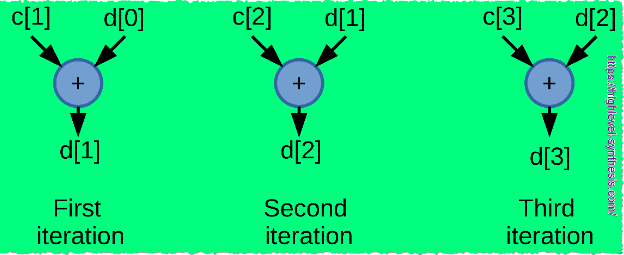
\includegraphics[scale=0.45,frame]{Figures/comb_loop/quiz_2_loop_graph}
\caption{Quiz 2 for loop graph}
\label{fig:comb_loop:quiz_2_loop_graph}
\end{figure}


These graph nodes should be executed one after another because of the data dependency between them. The dataflow graph in \autoref{fig:comb_loop:quiz_2_loop_execution} shows the hardware execution model of the \verb|for| loop.

\begin{figure}[h]
\centering
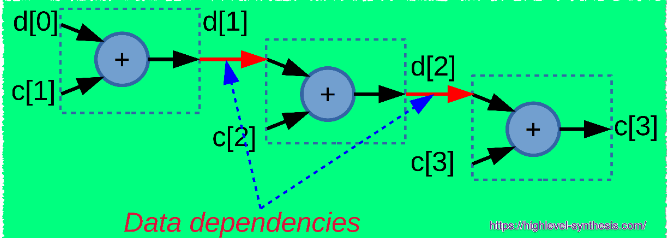
\includegraphics[scale=0.45,frame]{Figures/comb_loop/quiz_2_loop_execution}
\caption{Quiz 2 for loop execution}
\label{fig:comb_loop:quiz_2_loop_execution}
\end{figure}

\newpage
\section{Loop Unroll}

After presenting the concept of loop, let's see some actual code with some examples. We take $N$ bit binary adder shown in \autoref{fig:comb_loop:N_bit_binary_adder} (see \ref{sub:N_bit_binary_adder} for details). 


\begin{figure}[h]
\centering
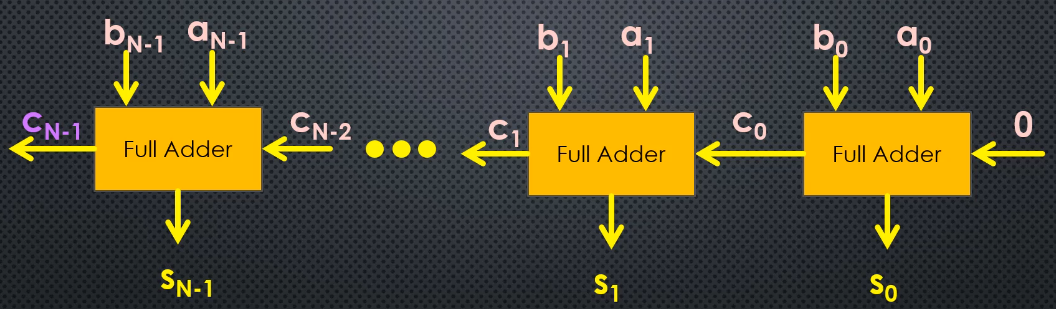
\includegraphics[scale=0.45,frame]{Figures/comb_loop/N_bit_binary_adder}
\caption{$N$ bit binary adder}
\label{fig:comb_loop:N_bit_binary_adder}
\end{figure}

The $N$ bit binary adder can be impelemted using \verb|for| loop as shown in \autoref{fig:comb_loop:loop_N_bit_adder}.

\begin{figure}[h]
\centering
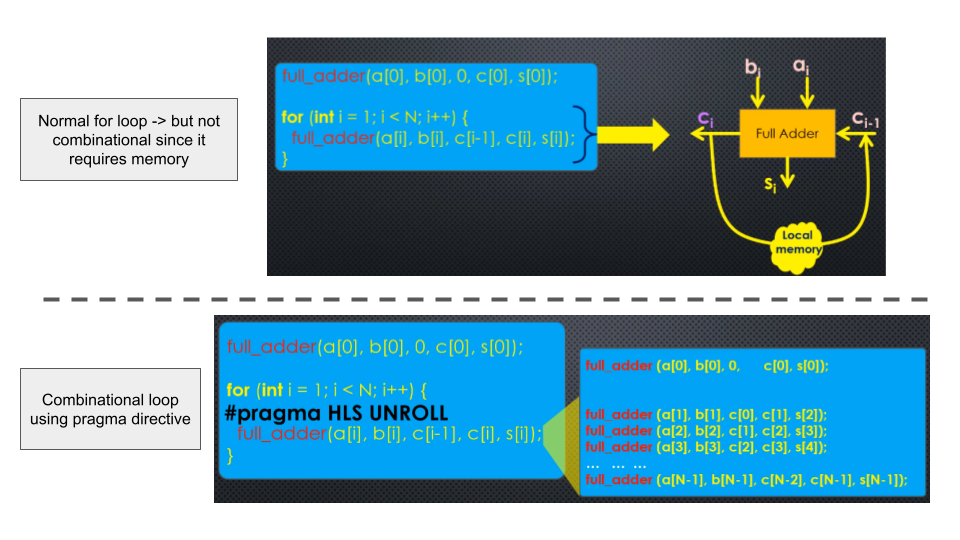
\includegraphics[scale=0.45,frame]{Figures/comb_loop/loop_N_bit_adder}
\caption{full-adder() function using for loop}
\label{fig:comb_loop:loop_N_bit_adder}
\end{figure}

\begin{itemize}

\item In the $\mathrm{1}^\mathrm{st}$ implementation, since we need the carry bit from the previous block, we need some kind of memory to track and save the result, resulting in a sequential circuit

\item To obtain a combinational circuit, we use the \verb|pragma unroll|, tell the \verb|for| loop to unroll the function \verb|full_adder()| and call it $N$ times, and no need for storage element

\end{itemize}

\subsection{Loop unroll condition}

Not every \verb|for| loop can be unrolled as shown in the $\mathrm{2}^\mathrm{nd}$ implementation in \autoref{fig:comb_loop:loop_N_bit_adder}. In order for the \verb|HLS| tool unroll a \verb|for| loop, the number of iteration need to be:

\begin{itemize}

\item known at compile time

\item in other words the number of iteration need to be bounded

\end{itemize}

\autoref{fig:comb_loop:loop_unroll_condition} shows some scenarios where a \verb|for| loop can be unrolled

\begin{figure}[h]
\centering
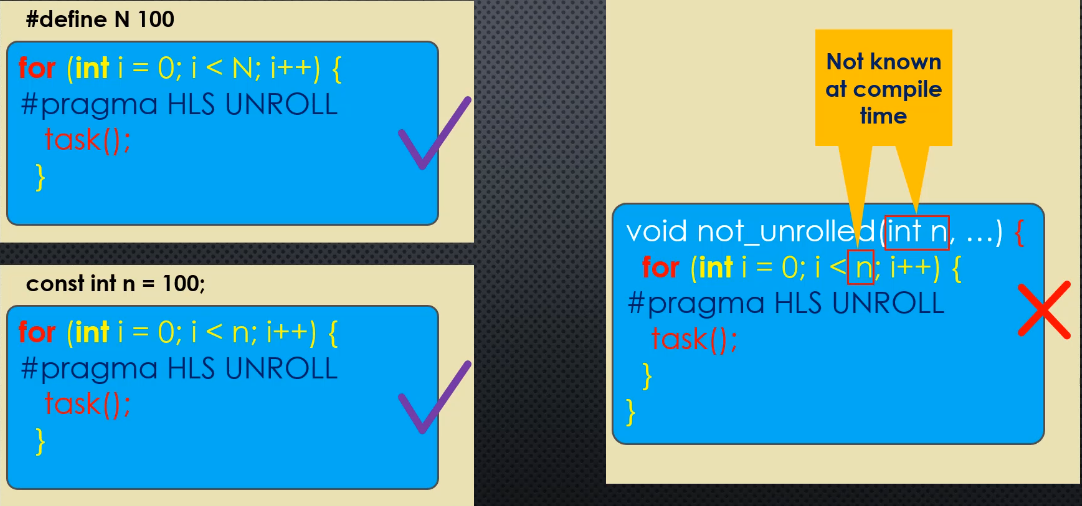
\includegraphics[scale=0.45,frame]{Figures/comb_loop/loop_unroll_condition}
\caption{Loop unroll condition}
\label{fig:comb_loop:loop_unroll_condition}
\end{figure}


\begin{itemize}

\item $\mathrm{1}^\mathrm{st}$ case \verb|N| is defined using a macro

\item $\mathrm{2}^\mathrm{nd}$ case \verb|n| is a variable but of type \verb|const|, so it can be unrolled

\item $\mathrm{3}^\mathrm{rd}$ case \verb|n| is a variable so it can be unrolled to combinational circuit

	\begin{itemize}
	\item \verb|HLS| tool will give a warning and sythethise the code into a sequential circuit
	\end{itemize}

\end{itemize}

\newpage
\subsection{Loop unroll resources}

When unrolling a \verb|for| loop, we need to be sure that the target FPGA has enough resources in order to implement the hardware needed for the \verb|for| loop.

That is because unrolling a \verb|for| loop, as done in \autoref{fig:comb_loop:loop_N_bit_adder}, result in different hardware instances.\\


\autoref{fig:comb_loop:loop_unroll_resources} shows an example of FPGA resources in terms of LUT.

\begin{figure}[h]
\centering
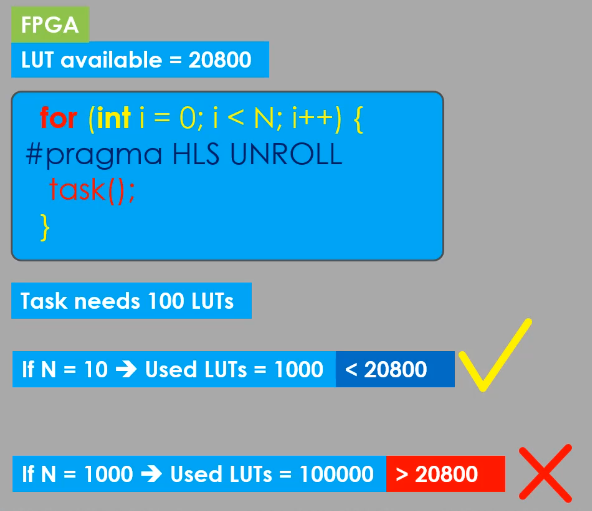
\includegraphics[scale=0.45,frame]{Figures/comb_loop/loop_unroll_resources}
\caption{Loop unroll resources}
\label{fig:comb_loop:loop_unroll_resources}
\end{figure}

\begin{itemize}

\item The \verb|task()| itself needs 100 LUT to be executed

\item So all depends on \verb|N|

	\begin{itemize}
	\item for \verb|N = 10|, we have enough resources
	
	\item for \verb|N = 100|,  the target FPGA lack of resources
	\end{itemize}

\end{itemize}

If the FPGA lack of resources, the synthesis tool (\verb|Vivado| in our case) complains and send some messages that it can't generate the bitstream file to program the FPGA.

\newpage
\subsection{Quiz}

\underline{Given:} which code in \autoref{fig:comb_loop:quiz_for_loop_combinational} can be synthesised into a combinational circuit ?


\begin{figure}[h]
\centering
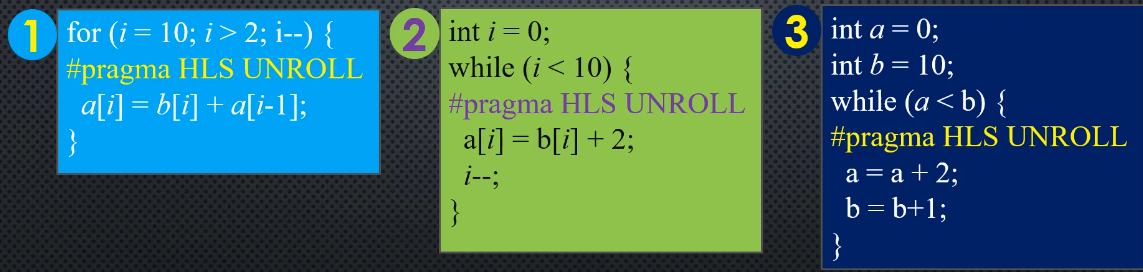
\includegraphics[scale=0.40,frame]{Figures/comb_loop/quiz_for_loop_combinational}
\caption{Quiz for loop}
\label{fig:comb_loop:quiz_for_loop_combinational}
\end{figure}

\underline{Solution:}

\begin{itemize}


\item The $\mathrm{1}^\mathrm{st}$ code can be synthesised into a combinational circuit as it has a static \verb|for| loop bound that can be determined at compile time 

\item The $\mathrm{2}^\mathrm{nd}$ code can also be synthesised into a combinational circuit as it has a static \verb|while| loop bound that can be determined at compile time

\item The $\mathrm{3}^\mathrm{rd}$ code cannot be synthesised into a combinational circuit as the loop bound determined as run-time based on the value assigned to a and b variables in each iteration.

\end{itemize}


\newpage
\section{Parity Bit}
\label{sec:parity_bit}

Now in this section we take a practical example to apply the loop mechanism seen so far in this chapter.\\

The parity bit is a technique to \tbi{detect a single bit error in binary data}. The binary bit stored in memory can undergoes some error during processing or transmission due to many phenomena (terrestrial radiations, magnetic fields,$\cdots$). The pheneomenon of error is so critical in many indsutries (nuclear, satellite,$\cdots$).\\


Single Event Upset (also known as soft-error) is one of the famous models representing this type of error. This model assumes that one of the binary bits changes its state from 0 $\rightarrow$ 1 or from 1 $\rightarrow$ 0 (as can be seen in \autoref{fig:comb_loop:parity_bit_intro}).

As an example, a Single Event Upset in the flight computers of Airbus A330 on 7 October 2008 is suspected to result in an aircraft upset that nearly ended in its crashing after the computers underwent several malfunctions.
  
\begin{figure}[h]
\centering
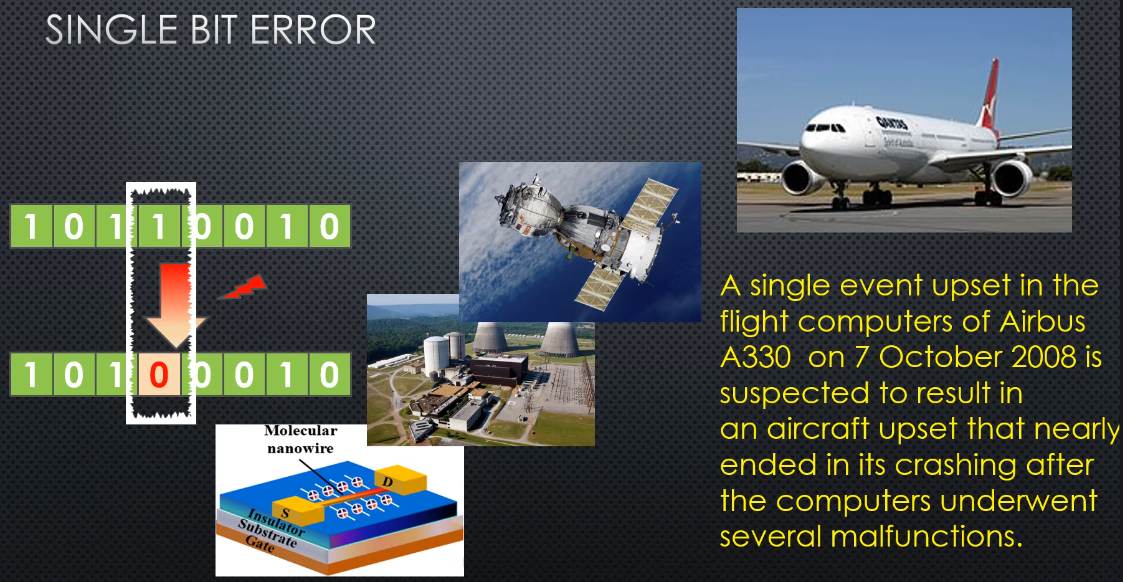
\includegraphics[scale=0.40,frame]{Figures/comb_loop/parity_bit_intro}
\caption{Parity bit and single event upset}
\label{fig:comb_loop:parity_bit_intro}
\end{figure}
 
\newpage
\subsection{Defintion of parity bit}

Now let's move to the defintion of this parity bit technique.

A parit bit is a one bit signature that is attached to the original $n$ bit data. The attachement can be doe via saving, or via transmission, and it is done by the parity generator.


\begin{figure}[h]
\centering
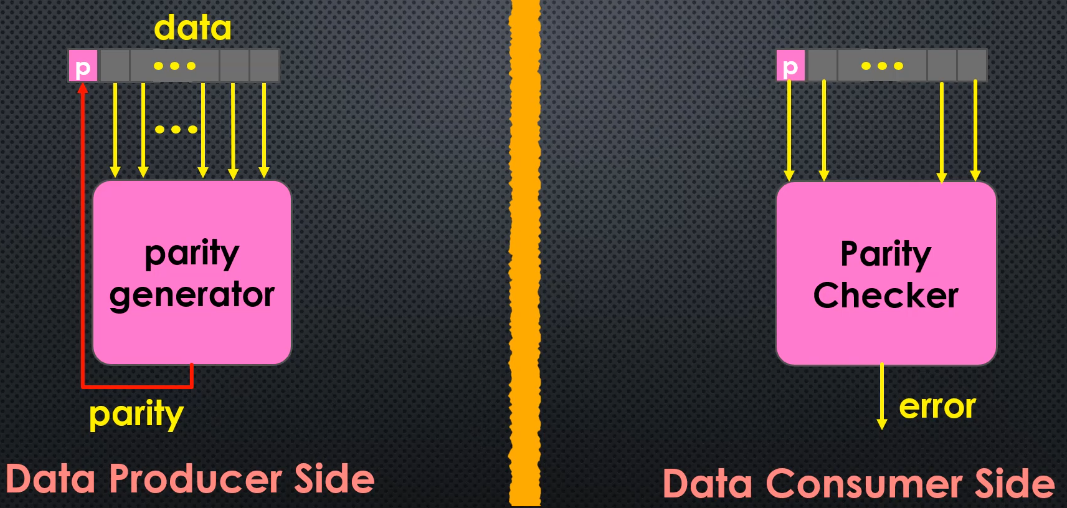
\includegraphics[scale=0.40,frame]{Figures/comb_loop/parity_bit_definition}
\caption{Parity bit definition}
\label{fig:comb_loop:parity_bit_definition}
\end{figure}

Then at the receiver side, the parity checker can check if we have some error in the data using this parity bit.

\newpage
\subsection{Parity types}

The parity is classified into 2 types: odd and even.

The general rule for odd or even is that the number of 1 in the data + parity bit should be even or odd. An example is shown in \autoref{fig:comb_loop:parity_types} to illustrate the concept.

\begin{figure}[h]
\centering
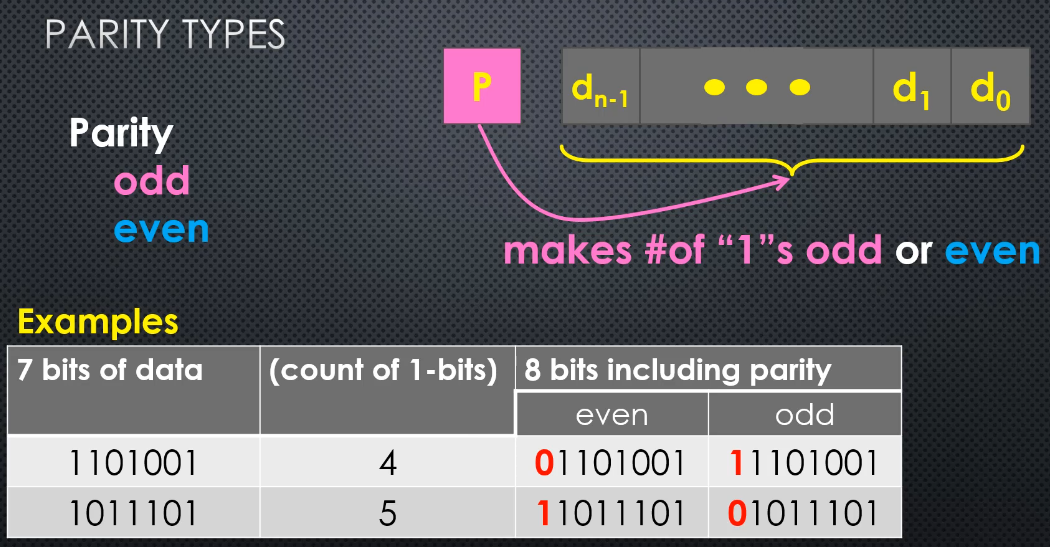
\includegraphics[scale=0.40,frame]{Figures/comb_loop/parity_types}
\caption{Parity types}
\label{fig:comb_loop:parity_types}
\end{figure}

\begin{itemize}

\item $\mathrm{1}^\mathrm{st}$ example where number of 1 $=$ 4

	\begin{itemize}
	\item If we want even parity, $\rightarrow$ parity bit should be 0 because 
	
	$ 4 \, (\,\text{in data}\,) \, + 0 \, = \, 4 \, (\,\text{even}\,)$
	
	\item If we want odd parity $\rightarrow$ parity bit should be 1 because 
	
	$ 4 \, (\,\text{in data}\,) \, + 1 \, = \, 5 \, (\,\text{odd} \,)$
	\end{itemize}

\item $\mathrm{2}^\mathrm{nd}$ example, number of 1 $=$ 5

	\begin{itemize}
	\item If we want even parity, the $\mathrm{8}^\mathrm{th}$ parity bit should be 1 because $5 \, + \ , 1 \, = \, 6 \, (\,\text{even}\,)$
	
	\item Same if we want for odd parity, he $\mathrm{8}^\mathrm{th}$ parity bit should be 0 because because 
	
	$5 \, + \ , 1 \, = \, 6 \, (\,\text{odd} \,)$

	\end{itemize}


\end{itemize}

\newpage
\subsection{Quiz}

The data in \autoref{fig:comb_loop:quiz_parity_bit} contain their parity bit , which one is erroneous ?

\begin{figure}[h]
\centering
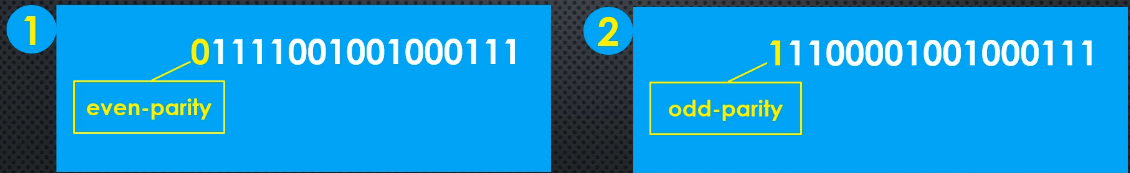
\includegraphics[scale=0.40,frame]{Figures/comb_loop/quiz_parity_bit}
\caption{Quiz parity bit}
\label{fig:comb_loop:quiz_parity_bit}
\end{figure}

\underline{Solution:}

\begin{itemize}

\item $\mathrm{1}^\mathrm{st}$ case: the data is erroneous as the number of ones in the data is 9, so then even parity should be 1, but it is 0

\item $\mathrm{2}^\mathrm{nd}$ case: this one also has an error as the number of ones is 7, so the odd-parity bit should be 0 but it is 1.

\end{itemize}

\todo{quiz parity bit} \uti{quiz parity bit:}

\begin{itemize}

\item \textit{To see later what is the purpose of this exercice}

\item \textit{In my mind, I thaught we should correct the original data, not the parity bit itself}

\item \textit{To ask some AI about this exercice}

\end{itemize}


\newpage
\section{Parity Bit Design}
\label{sec:parity_bit_design}

After understanding the concept of parity bit in \autoref{sec:parity_bit}, we move to the desing part.

\autoref{fig:comb_loop:parity_design} shows desing for parity bit for 2 $(\,d_0 \, , \, d_1\,)$ and 3 bit $(\,d_0 \, , \, d_1\, , \, d_2)$ data. 

\begin{figure}[h]
\centering
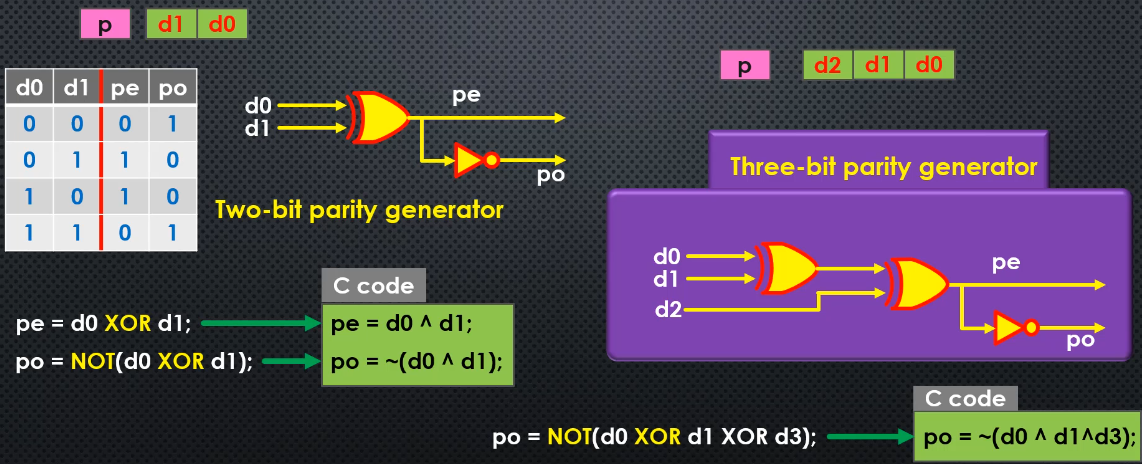
\includegraphics[scale=0.40,frame]{Figures/comb_loop/parity_design}
\caption{Parity bit design for 2 and 3 bit}
\label{fig:comb_loop:parity_design}
\end{figure}

\begin{itemize}

\item The output of the system in the truth table is $p_e$ (for parity even) and $p_o$ (for parity odd)

\end{itemize}

\todo{parity 3 bit desing} \uti{parity 3 bit desing:}

\begin{itemize}

\item \textit{To  derive the truth table for the 3 bit case as in exercice, similar to the 2 bit case}

\item \textit{To do after reviewing the combinational circuit part, and to do it with the VHDL course}

\end{itemize}

Now generalizing the desing concept from 2 or 3 bit to $W$ bit, can be done using a chain of \verb|XOR| gates, as shown in \autoref{fig:comb_loop:parity_w_bit}.

\begin{figure}[h]
\centering
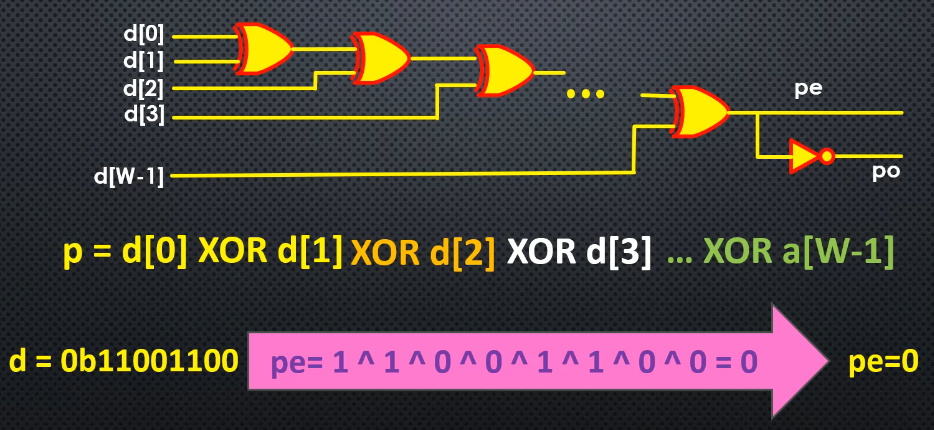
\includegraphics[scale=0.40,frame]{Figures/comb_loop/parity_w_bit}
\caption{Parity bit for $W$ bit data}
\label{fig:comb_loop:parity_w_bit}
\end{figure}

As for the propagation delay $t_p$ for the implementation of \autoref{fig:comb_loop:parity_w_bit}, assuming each \verb|XOR| gate has $\delta$ delay, and we have $(W \, - \, 1)$ \verb|XOR| gate (each 2 data bit line $d[w]$ and $d[\, w + \, 1]$ need 1 \verb|XOR| gate, so for $W$ data bit lines we need $(\, W\, - \, 1\,)$ \verb|XOR| gates ), the total propagation delay is: 

\begin{equation}
t_p \, = \, (W \, - \, 1) \, \delta
\label{eq:tp_parity_bit}
\end{equation}

\subsection{Desing optimization}
\label{sub:design_optim}

\autoref{fig:comb_loop:parity_w_bit} desing can be optimized in terms of $t_p$. Assuming that $W$ is a power of $n$, that is $W \, = \, 2^n$, and due to the assoicativity and commutativity of the \verb|XOR| gates, a balance tree can implement the parity bit generator as shown in \autoref{fig:comb_loop:parity_w_bit_balance_tree}.


\begin{figure}[h]
\centering
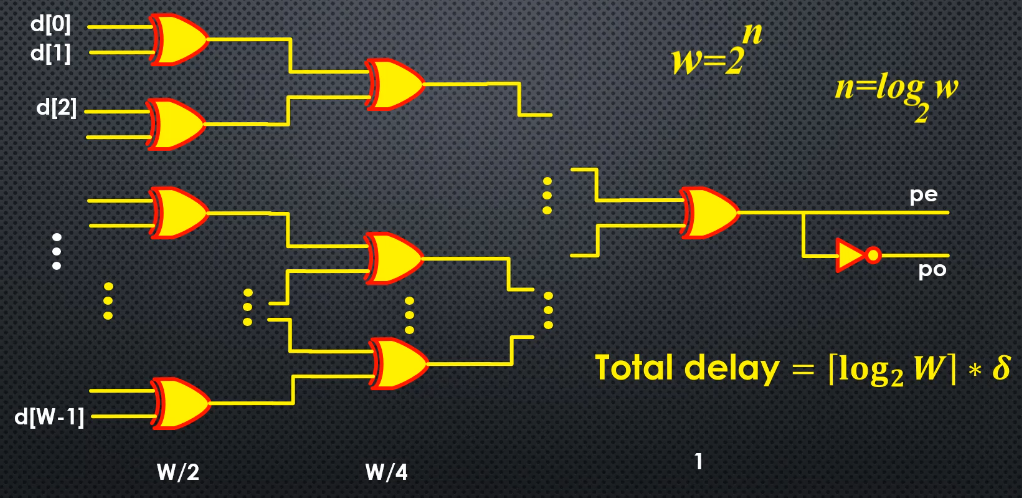
\includegraphics[scale=0.40,frame]{Figures/comb_loop/parity_w_bit_balance_tree}
\caption{Parity bit using balance tree}
\label{fig:comb_loop:parity_w_bit_balance_tree}
\end{figure}

This desing reduce $t_p$ to a function of $\log_2(W)$, which is much smaller than the one in \autoref{eq:tp_parity_bit}.


\begin{equation}
t_p \, = \, \lceil \log_2(W) \rceil \, \times \, \delta
\end{equation}


\newpage
\subsection{Quiz}
\label{sub:quiz_parity_bit}


\underline{Quiz 1:} If we assume $W \, = \, 1024$ bit,

\begin{enumerate}

\item What is number of levels (depth, or layers) of the final balanced tree ?

\item How many \verb|XOR| gates make the final hardware desing ?

\end{enumerate}

\underline{Solution Quiz 1:}

\begin{enumerate}

\item Number of layers equal to $\log_2(1024) \, = \, 10$ levels. 

\item Number of \verb|XOR| gates $1024 \, - \, 1 \, = \, 1023$ 

\end{enumerate}

The final desing for $W \, = \, 1024$ bit is shown in \autoref{fig:comb_loop:quiz_1_parity_bit_param}.

\begin{figure}[h]
\centering
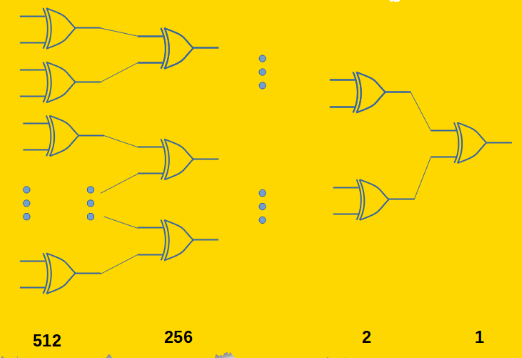
\includegraphics[scale=0.45,frame]{Figures/comb_loop/quiz_1_parity_bit_param}
\caption{Parity bit using balance tree}
\label{fig:comb_loop:quiz_1_parity_bit_param}
\end{figure}


\newpage
\underline{Quiz 2:} Find $t_p$ of an even parity bit generator for an 11 bit data if the delay of an \verb|XOR| gate is 1 ns.\\

\underline{Solution Quiz 2:} \\

\autoref{fig:comb_loop:quiz_11bit_parity} shows the desing using a balanced tree approach for 11 bit data line. 


\begin{figure}[h]
\centering
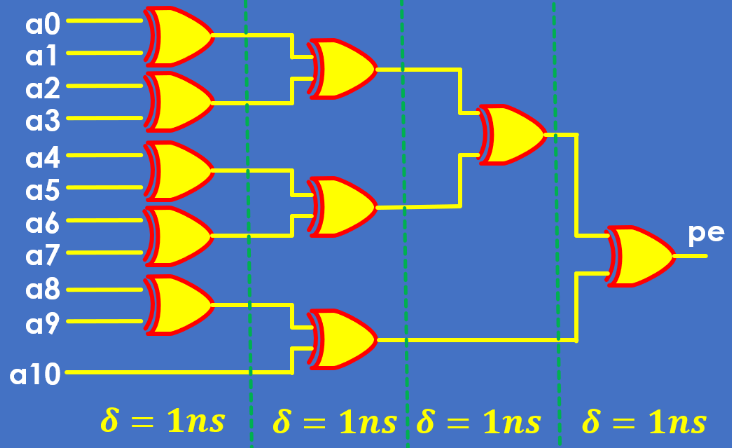
\includegraphics[scale=0.45,frame]{Figures/comb_loop/quiz_11bit_parity}
\caption{Parity bit using balance tree}
\label{fig:comb_loop:quiz_11bit_parity}
\end{figure}

Since the balance tree use a layer approach, each layer has a 1 ns delay even if in 1 layer we have multiple \verb|XOR| gates, where

\begin{itemize}

\item Total number of \verb|XOR| gates $ = \, W \, - \, 1 $

\item Number of \verb|XOR| gates per layer $ = \, \lfloor \displaystyle\frac{W}{2} \rfloor $. 

\end{itemize}

Thus total delay is $t_p \, = \, $ number of layers used $\times$ 1 ns $= \, 4 \, \times \, 1\, = \, 4$ ns.


\newpage
\section{Parity bit in HLS}

Recall from \autoref{sec:parity_bit_design}, that the generalized expression for $W$ bit data lines $d[w]$, take the form of:

\verb|p = d[0] XOR d[1] XOR d[2] ... XOR d[w - 1]|.

The implementation in \verb|HLS| is shown in \autoref{fig:comb_loop:parity_bit_hls}.

\begin{figure}[h]
\centering
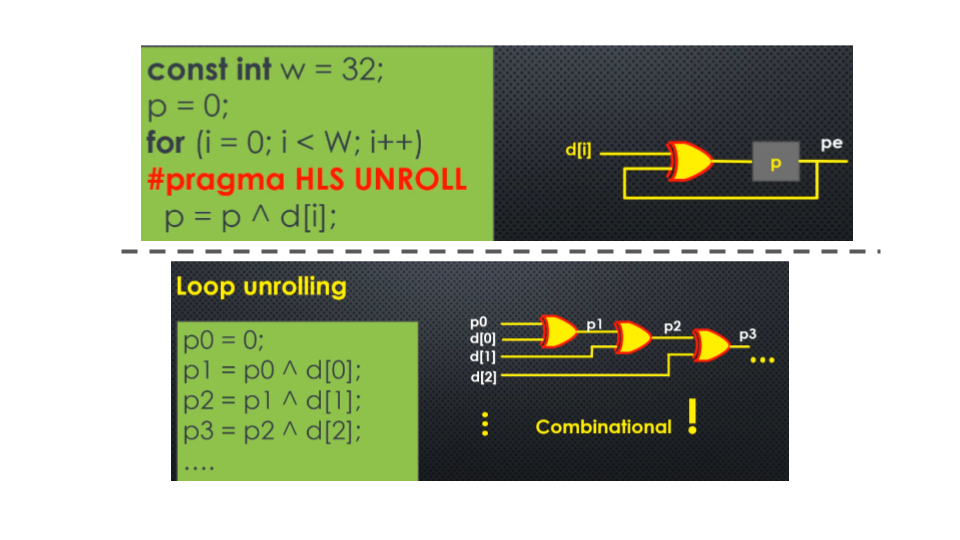
\includegraphics[scale=0.45,frame]{Figures/comb_loop/parity_bit_hls}
\caption{Parity bit HLS implementation}
\label{fig:comb_loop:parity_bit_hls}
\end{figure}

Notice that we use the \verb|#pragma HLS UNROLL| to unroll the \verb|for| loop. By unrolling the \verb|for| loop, we have an equivalent implementation (as shown in the bottom part of \autoref{fig:comb_loop:parity_bit_hls}), where \verb|HLS| tool copy automatically the body of loop statement in each iteration, which result in running the loop statements concurrently and not sequentially.

Whithout the \verb|pragma|, the parity bit by nature needs a result from previous iteration, thus it need some memory to track and save the result, which result in a non-combinational loop.\\

\underline{Note:} In the bottom part of \autoref{fig:comb_loop:parity_bit_hls}, the manually unrolled loop result in a ladder of \verb|XOR| gates, but \verb|HLS| tools handles automatically an optimized impelementation as the balanced tree seen in \ref{sub:design_optim}.


\subsection{Some Work to be done}

\todo{Project Parity-Bit-Vitis} \uti{Project Parity-Bit-Vitis:}

\begin{itemize}

\item \textit{To run the simulation later using Vivado, because in the course it wasn't done}

\item \textit{There is also the usage of the wavefrom viewer, and see for each input we have the correct output}

	\begin{itemize}
	
	\item \textit{I didn't understant this quiet right}	
		
	\item \textit{to be re-done this later}

	\end{itemize}

\end{itemize}

\todo{Waveform viwer in Vitis} \uti{Waveform viwer in Vitis:}

\begin{itemize}

\item \textit{To understand how to use the waveform viwer in Vitis}

\item \textit{How to use with some combinational circuit for example}

\end{itemize}


\newpage
\section{Extra Exercices}

\begin{enumerate}

\item Describe a combinational circuit is HLS to find the even-parity bit of all even bits in an $N$ bit binary data.

\item Describe a combinational circuit in \verb|HLS| to count the number of ones in an $N$ bit binary number. (For example $N\, = \, 345$)

\item Design a combination circuit that returns the even-parity bit of all even bits of a 234-bit input binary number. 

Do not use \verb|for| loop statement. 

\end{enumerate}





\newpage
\section{Summary Combinational Loops}

\begin{itemize}

\item Prallelism and delay:

	\begin{itemize}
	\item A nice demo to illustrate the concept of parallelism and delay is in \ref{eq:tp_parity_bit}
	
	\item The intuition of the exercices is that due to the parallelism properties in FPGA hardware and in the balanced tree desing for parity bit system, $t_p$ is not multiplied, or for example equal to the number of \verb|XOR| gates used in the system
	
	\item \todo{Prallelism and delay} \uti{Prallelism and delay}: 
	
	\textit{To review this concept later, and that I understood this well, when reviewing the logic desing course and VHDL course}
	
	
	\end{itemize}


\end{itemize}












\chapter{Integer Arithmetic}

\section{Introduction}

This chapter is a continuity for \autoref{chap:data_types}, where we explain how \verb|HLS| provide support for arithmetic operations, which takes much more efficient in \verb|HDL|.\\

\todo{Intro Integer Arithmetic} \uti{Intro Integer Arithmetic:}

\begin{itemize}

\item \textit{To re-write later the intro, after reviewing the number system from logic desing course, and finishing this chapter}

\end{itemize}

\newpage
\section{Definition}

Basic arithmetic operator (from addition,subtraction,$\cdots$) are shown in \autoref{fig:int_arithmetic:arith_operator}. 

\begin{figure}[h]
\centering
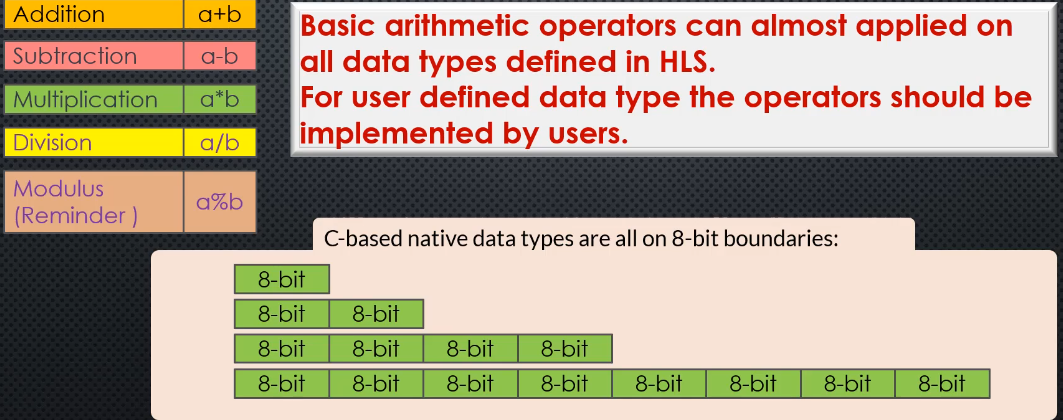
\includegraphics[scale=0.4,frame]{Figures/int_arithmetic/arith_operator}
\caption{Basic Arithmetic Operator}
\label{fig:int_arithmetic:arith_operator}
\end{figure}

These operator can be applied on all native \verb|C| and \verb|C++| data types, and on arbitrary widht data types. Notice that for \verb|C| data types, data type width are multiple of 8 bit, thus operator accuracies are constrained by these boundaries.\\

\todo{operator accruacy} \uti{operator accruacy:}

\begin{itemize}

\item \textit{To see what is that operator accuracy mean, and where it can be applied on. For example:}

	\begin{itemize}
	\item \textit{is there some relation with round off, or truncating error }
	
	\item \textit{the overflow concept also, like the surpassing the capacity of certain range}	
	
	
	\end{itemize}

\end{itemize}

\newpage
Beside from bit width, arithmetic operation can be applied on same data type or different data type, as shown in \autoref{fig:int_arithmetic:arith_operator_data_type}.

\begin{figure}[h]
\centering
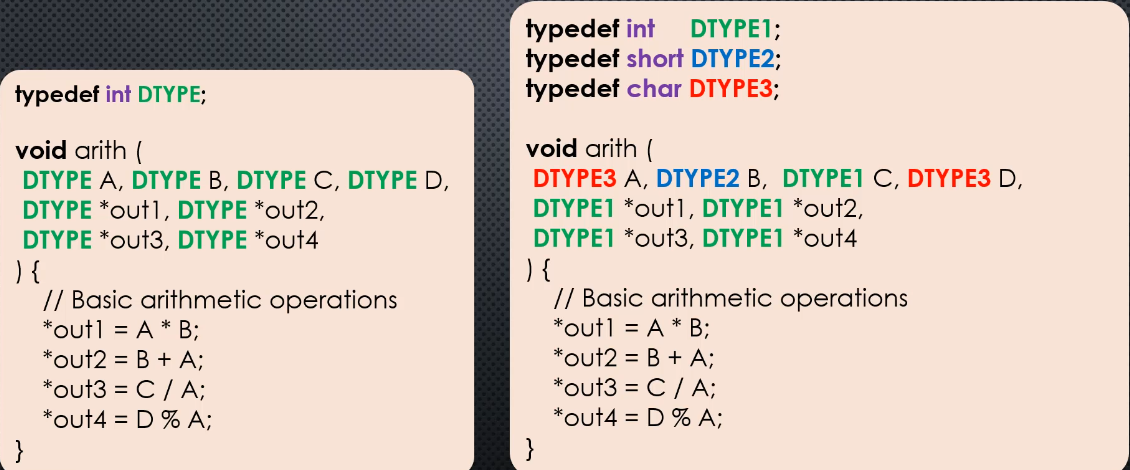
\includegraphics[scale=0.4,frame]{Figures/int_arithmetic/arith_operator_data_type}
\caption{Basic Arithmetic Operator on same or different data type}
\label{fig:int_arithmetic:arith_operator_data_type}
\end{figure}

\begin{itemize}

\item $\mathrm{1}^\mathrm{st}$ example use same data type (\verb|int|) for all argument of the function

\item $\mathrm{2}^\mathrm{nd}$ example uses 3 different data type (\verb|int|,\verb|short| and \verb|char|)

\end{itemize}

\verb|HLS| impelement these operation through \tbi{automatic type casting}.\\

\newpage
\subsection{Circuit types: sequential vs combinational}
\label{sub:circuit_types}

Since in \autoref{part:fundamentals} until now we focus on combinational circuit, we expect that combinational circuit implement arithmetic operation on any data type.

Now let's take a look to what type of operator we have in \verb|HLS| tool as \verb|Vitis|. We have 2 types (shown in \autoref{fig:int_arithmetic:arith_operator_circuit}): combinational and pipeline.

\begin{figure}[h]
\centering
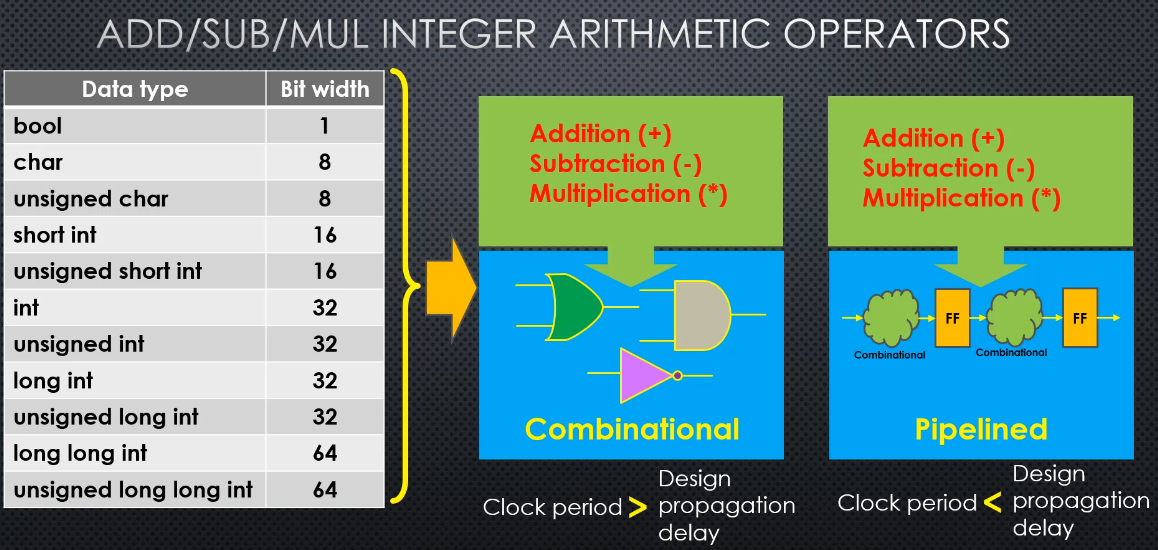
\includegraphics[scale=0.4,frame]{Figures/int_arithmetic/arith_operator_circuit}
\caption{Arithmetic operator and their impelementation}
\label{fig:int_arithmetic:arith_operator_circuit}
\end{figure}

Pipepline circuit uses flip flop (sequential) circuit to minimize $t_p$, and these will be covered in \autoref{part:sequential}.

\todo{Citing Next Part} \textit{Citing Next Part:}

\begin{itemize}

\item \textit{To see how to solve this issue of referecning part of reports}

\end{itemize}

\newpage
There are 2 constraint in choosing between combinational and sequential desing as shown in \autoref{fig:int_arithmetic:circuit_constraint}: the clock period and resources.

\begin{figure}[h]
\centering
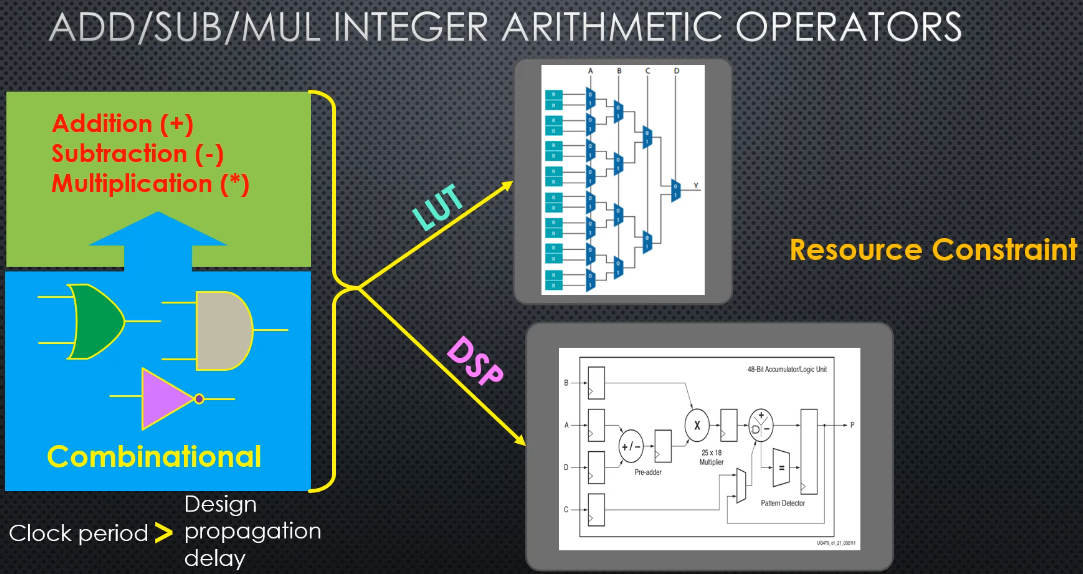
\includegraphics[scale=0.4,frame]{Figures/int_arithmetic/circuit_constraint}
\caption{Circuit Constraint}
\label{fig:int_arithmetic:circuit_constraint}
\end{figure}

\begin{itemize}

\item If the clock period is bigger than the period of arithmetic operations, than combinational circuit is syntehsised

\item Otherwise, sequential circuit is used

\end{itemize}


\newpage
\section{Operator Overloading}

In this section we see how \verb|HLS| uses operator overloaing to apply arithmetic operator on arbitrary precision data type.\\

As a recall, operator overloading is a concept from software programming which adds new implementation based on its argument types. The goal it to use that same operator whith its same standard notation and apply it on the new data type.\\


\autoref{fig:int_arithmetic:op_overloading_hls} shows examples for operator overloading.

\begin{figure}[h]
\centering
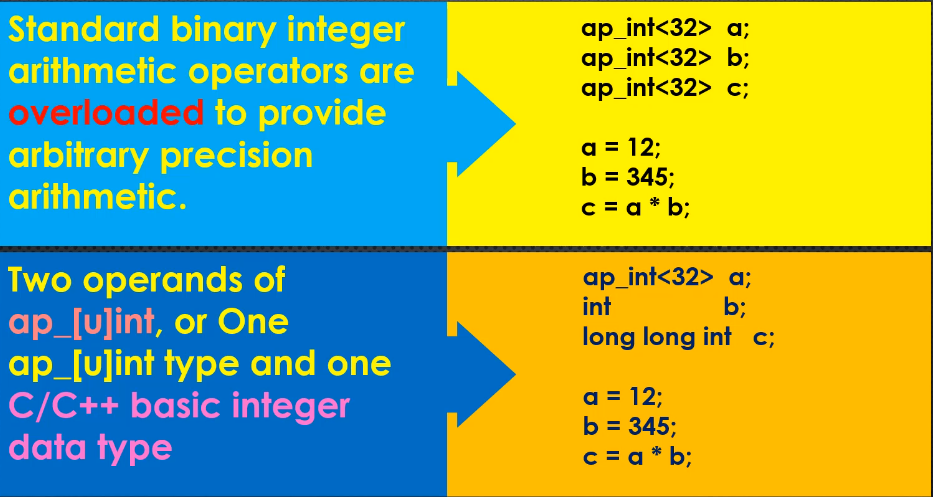
\includegraphics[scale=0.4,frame]{Figures/int_arithmetic/op_overloading_hls}
\caption{Operator Overloading in HLS}
\label{fig:int_arithmetic:op_overloading_hls}
\end{figure} 


\begin{itemize}

\item $\mathrm{1}^\mathrm{st}$ example declare variables of 32 bit width, than use \verb|=| operator to assign some values.

Then there is the usage of \verb|*| operator to do a normal multiplication.

\item $\mathrm{2}^\mathrm{nd}$ example shows how \verb|HLS| uses overloading to accept operand of different type: arbitrary width data type and standard data type from \verb|C| or \verb|C++| language. 

\end{itemize}

\newpage
\autoref{fig:int_arithmetic:op_overloading_function_code} shows example along with functions, where we have the same body but different argument, along with some performance measure after sythesis.

\begin{figure}[h]
\centering
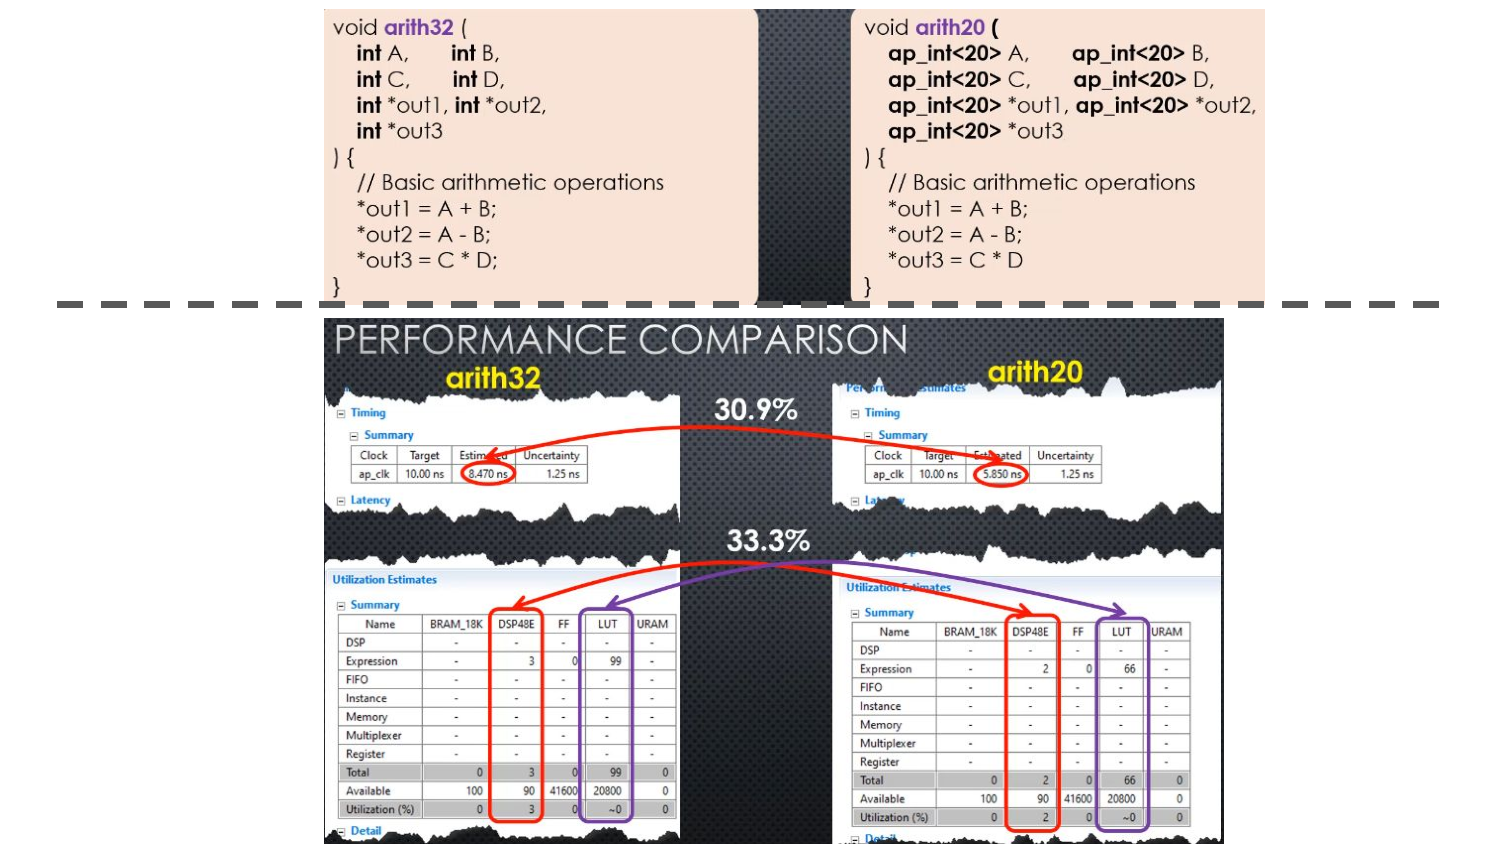
\includegraphics[scale=0.65,frame]{Figures/int_arithmetic/op_overloading_function_code}
\caption{Operator Overloading with functions}
\label{fig:int_arithmetic:op_overloading_function_code}
\end{figure} 

The function with 20 bit data types uses less resources in general.

\subsection{Quiz}

\underline{Given:} Compare the synthesis report of the \verb|HLS| code in \autoref{fig:int_arithmetic:quiz_op_overloading}, for 23 bit datay type and \verb|int| data type.

\begin{figure}[h]
\centering
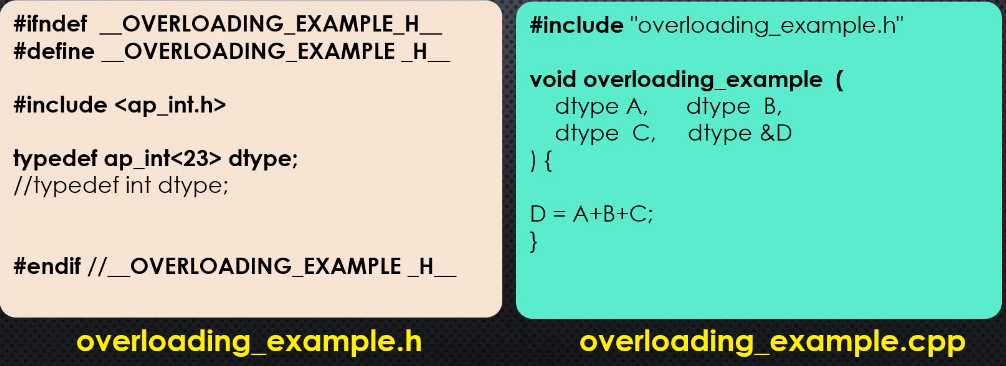
\includegraphics[scale=0.35,frame]{Figures/int_arithmetic/quiz_op_overloading}
\caption{Quiz Operator Overloading}
\label{fig:int_arithmetic:quiz_op_overloading}
\end{figure} 

\newpage
\section{Timing Constraint}


The synthesis of arithmetic expressions into combinational circuit is influenced by the timing constraint of the desing. 


Timing constraint contains 2 elements as shown in \autoref{fig:int_arithmetic:time_constraint}:  

\begin{figure}[h]
\centering
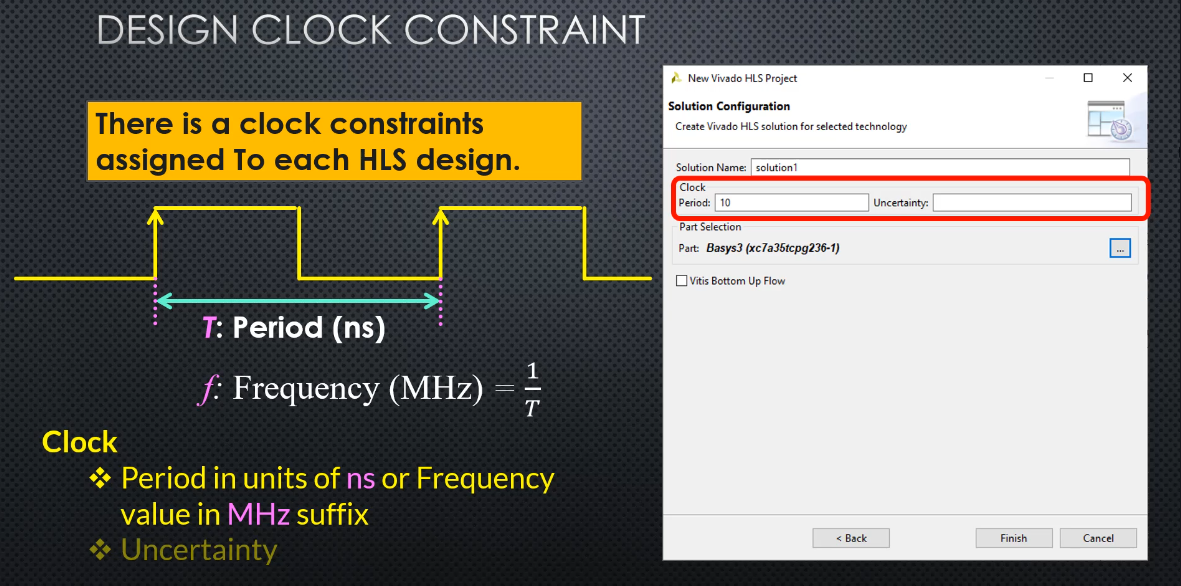
\includegraphics[scale=0.35,frame]{Figures/int_arithmetic/time_constraint}
\caption{Timing constraint: clock period and uncertainty}
\label{fig:int_arithmetic:time_constraint}
\end{figure} 

\begin{itemize}

\item Clock period, which comes in ns for FPGA project or MHz in terms of frequency

\item Uncertainty, which will be covered in part 2 of the course

\end{itemize}


\newpage
Recall from \ref{sub:circuit_types} that the synthesis of digital circuit is related to the clock period and $t_p$. 

\autoref{fig:int_arithmetic:time_constraint_example} presents an example of multiplication function for 2 clock period option: 10 ns (the default one), and the $\mathrm{2}^\mathrm{nd}$ one is chosen to be 5 ns.


\begin{figure}[h]
\centering
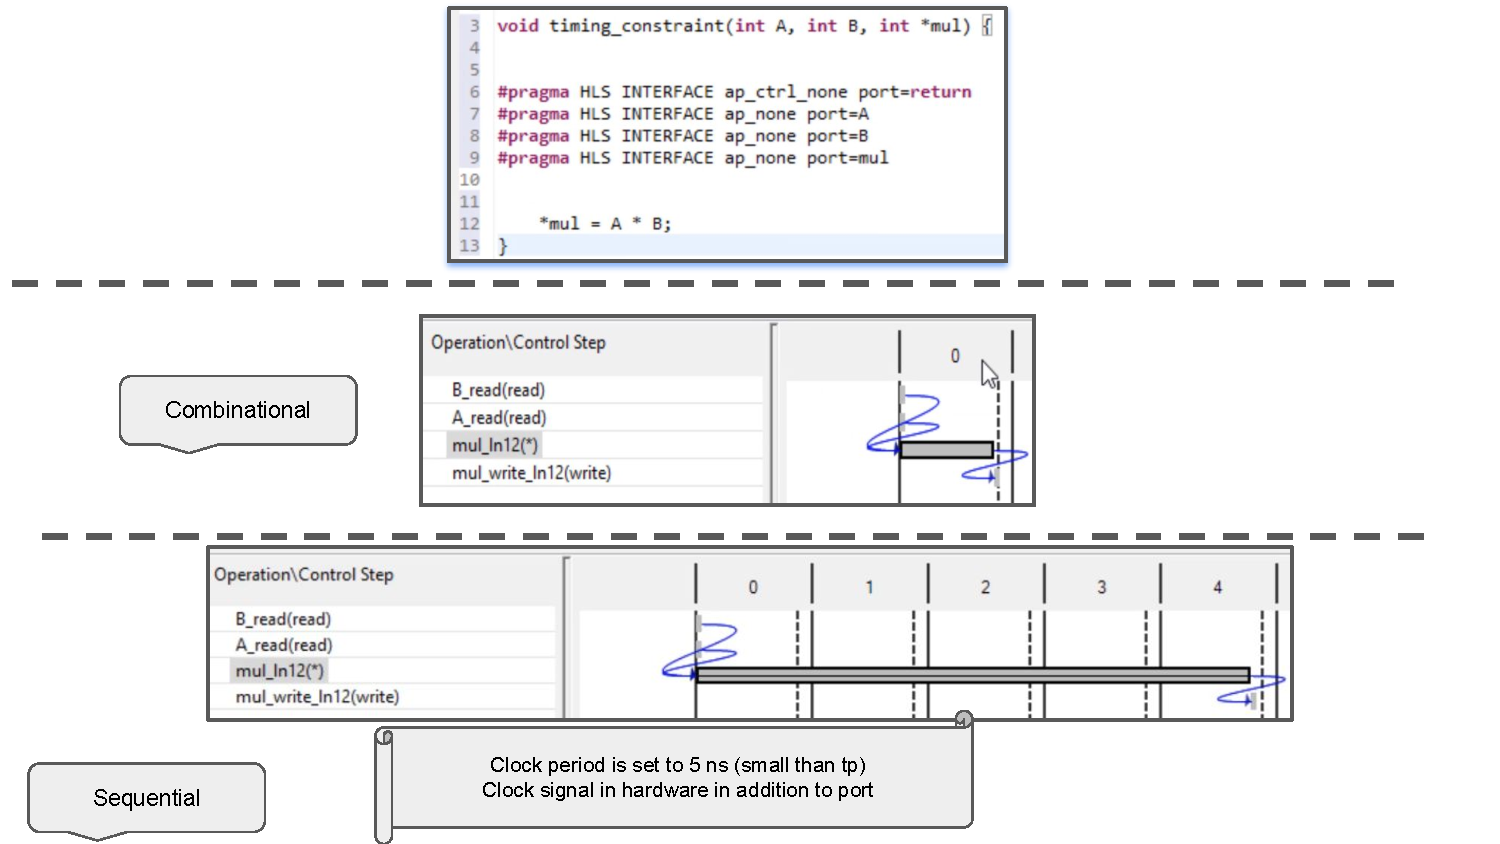
\includegraphics[scale=0.60,frame]{Figures/int_arithmetic/time_constraint_example}
\caption{Timing constraint: clock period and uncertainty}
\label{fig:int_arithmetic:time_constraint_example}
\end{figure}

For the 5 ns, we see that using the analysis perspective that the operation is composed to 5 steps, and it used some memory elements to transfer data between the operations.\\

\todo{Analysis perspective} \uti{Analysis perspective:}

\begin{itemize}

\item \textit{To see how, and train on it, how to use this analysis perspective in Vitis}

\item \textit{Its role in HDL in general, and apply it to HLS}

\end{itemize}


\newpage
\subsection{Quiz}

\underline{Given:} Find a proper value for the clock period to sythesis the code of \autoref{fig:int_arithmetic:quiz_timing_constraint} into a combinational circuit.


\begin{figure}[h]
\centering
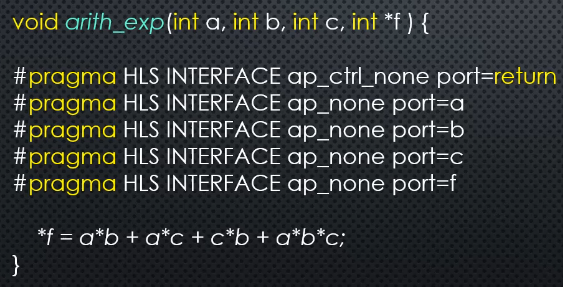
\includegraphics[scale=0.60,frame]{Figures/int_arithmetic/quiz_timing_constraint}
\caption{Quiz timing constraint}
\label{fig:int_arithmetic:quiz_timing_constraint}
\end{figure}

\underline{Solution:} read TimingConstraints-Quiz-Solution.pdf.

\newpage
\section{DSP Resources}

To implement arithmetic expressions, FPGA comes traditionally with LUT, which works under simple scenarios. But for applications wich requires more computaitonal demands, FPGA vendors introduces DSP blocks, wihch have high performance for complex computation task.

\begin{figure}[h]
\centering
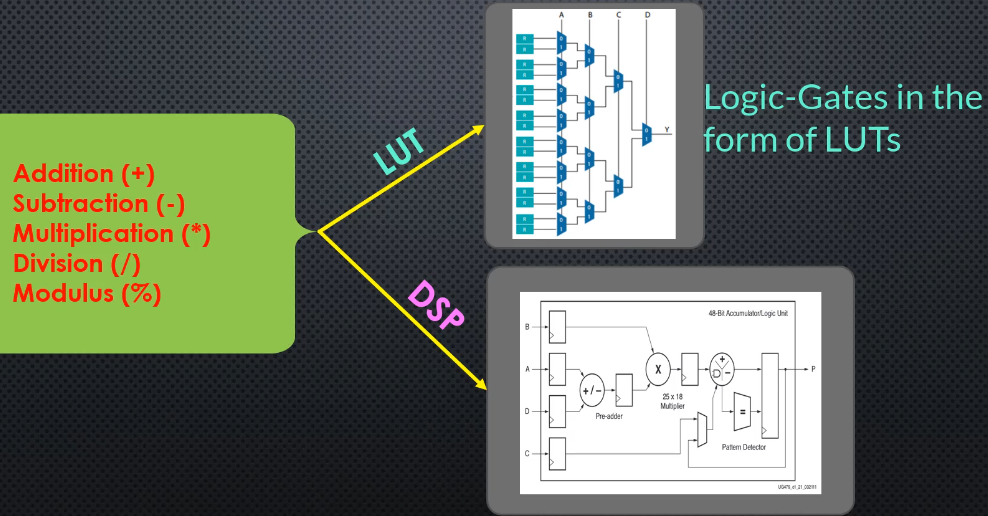
\includegraphics[scale=0.40,frame]{Figures/int_arithmetic/arithmetic_resources}
\caption{Arithmetic Resources}
\label{fig:int_arithmetic:arithmetic_resources}
\end{figure}

A typical DSP block receives a couple of inputs and then passes them through a set of pre-designed reconfigurable
addition and multiplication modules. \autoref{fig:int_arithmetic:DSP48_block} shows a DSP48 block which is used in \verb|Basys3| board.


\begin{figure}[h]
\centering
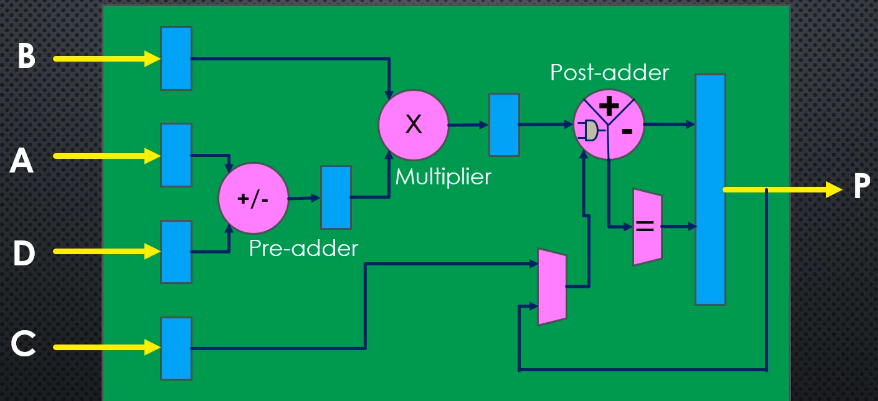
\includegraphics[scale=0.40,frame]{Figures/int_arithmetic/DSP48_block}
\caption{DSP Block}
\label{fig:int_arithmetic:DSP48_block}
\end{figure}

\verb|HLS| tools usually automate all computation steps, but havving some familiarity with mechanism inside the DSP block help us to guide us for the synthesis process to generate high performance RTL descirption.\\

\todo{DSP block and RTL description} \uti{DSP block and RTL description:}

\begin{itemize}

\item \textit{To see later when starting the VHDL course, the role of FPGA block in general, like the LUT, DSP,memories,$\cdots$}

	\begin{itemize}
	\item \textit{Try to see some resources like papers, github,$\cdots$ to see how to simulations and study to optmize these resources}
	\end{itemize}

\end{itemize}

\subsection{DSP description}

\begin{itemize}

\item At the heart of the DSP, there is a multiplier that accepts a 25 bit and an 18 bit two's complement
inputs and generates a 43 bit two's complement result.

\item This multiplier receives one of its inputs via a pre adder module and gives its output to a post adder
module.

\item There are also other paths in a DSP to provide enough data path to implement different mathematical
and logical expressions.

\item Most data paths inside the DSP can be registered in flip flops.

\item In addition, the multiplier and additions inside the DSP can be implemented by a single stage combinational circuit or a multi-stage pipeline structure.

\end{itemize}

\todo{DSP description} \uti{DSP description:}

\begin{itemize}

\item \textit{There are to much theory, to see later some other resources to understand them}

\end{itemize}

\newpage
\subsection{DSP Example}

Let's see now how a DSP can be reconfigured using the 2 cases of \autoref{eq:dsp_example}.

\begin{equation}
\begin{array}{rcl}
f \, &=& \, A \, \star \, B \\
f \, &=& \, (A \, + \, B) \, \star \, D 
\end{array}
\label{eq:dsp_example}
\end{equation}

\autoref{fig:int_arithmetic:dsp_example} shows their graph representation along with the data path in for each DSP block.

\begin{figure}[h]
\centering
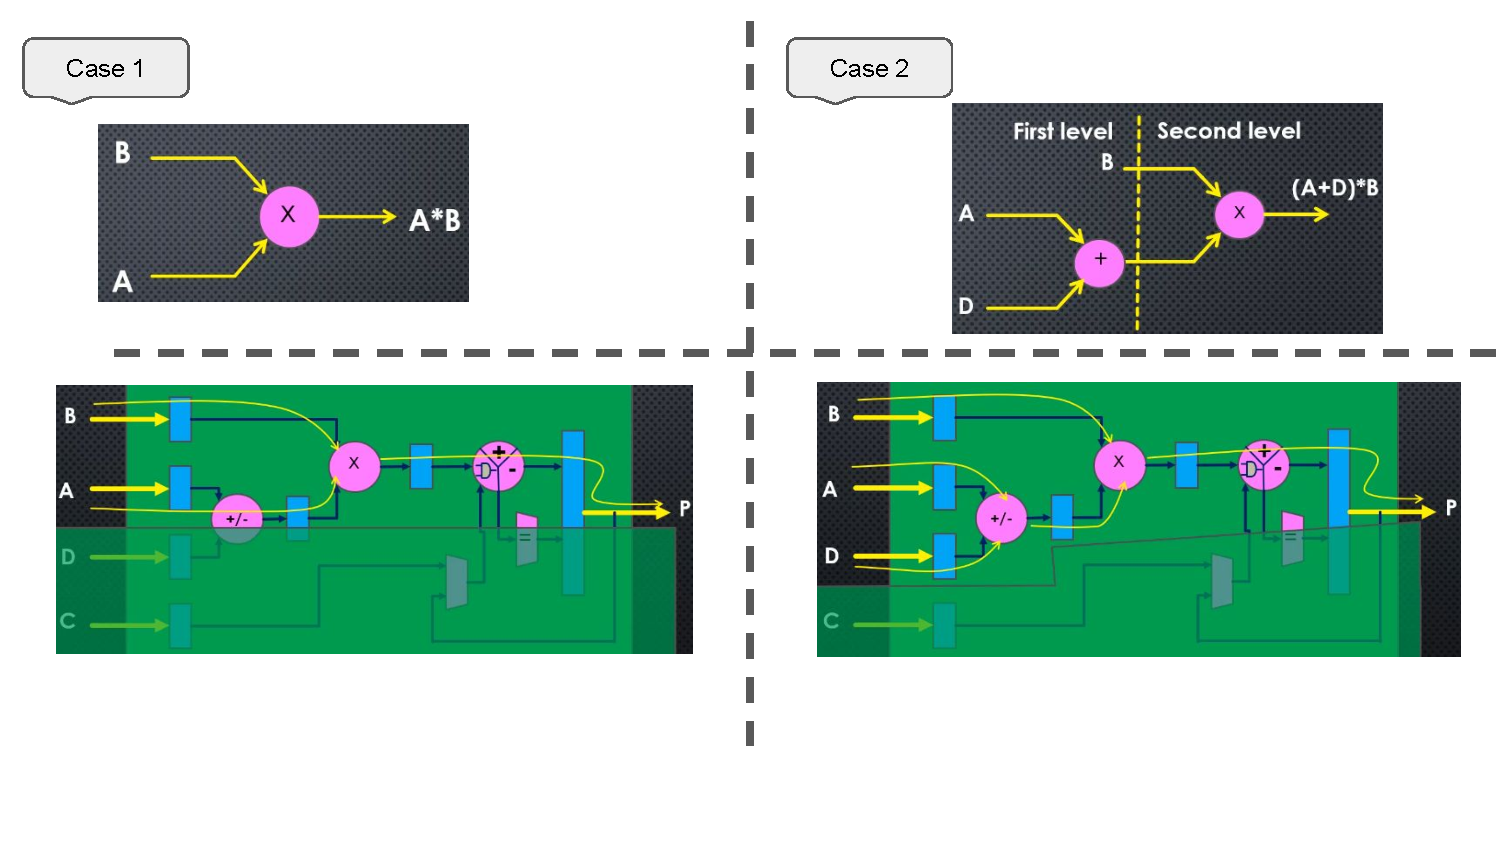
\includegraphics[scale=0.55,frame]{Figures/int_arithmetic/dsp_example}
\caption{DSP Example}
\label{fig:int_arithmetic:dsp_example}
\end{figure}


\begin{itemize}

\item \underline{Case 1:} $B$ input feeds the multiplier directly.

$A$ bypasse the adder and it is connected to the multiplier

Finally, the multipler result gets to the output by avoinding all the operators along the path 

\item \underline{Case 2:} Same principle as in case 1, but this epxression has 2 level in its graph

\end{itemize}


\todo{DSP Examples} \uti{DSP Examples:}

\begin{itemize}

\item \textit{Is there any relation between the graph and the DSP ? maybe concerning its path}

	\begin{itemize}
	\item \textit{To be seen later}
	\end{itemize}

\item \textit{Can we implement epxression with more than 4 inputs to this DSP48 block?}

	\begin{itemize}
	\item \textit{Maybe need more complex DSP}
	
	\item \textit{Or this DSP48 can reconfigure and evolve to handle more complex expresssions}
	
	\item \textit{To be seen later}
	\end{itemize}

\end{itemize}


\newpage
\section{Resource Selection}

We saw that the implementation of arithmetic and logic expression can be done via 2 resources: LUT and DSP blocks. In this section we see how to guide the synthesis tools to choose between these 2 resources.\\


In order to implement \verb|C/C++| code into hardware resources, \verb|Vitis| perform 2 task: elaboration and mapping.

\begin{figure}[h]
\centering
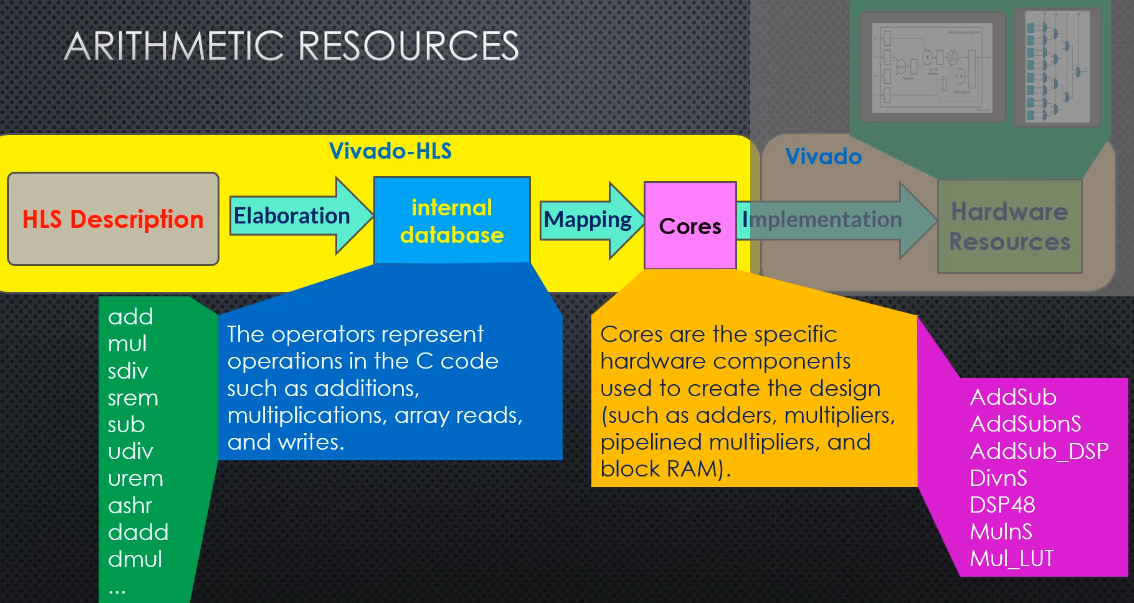
\includegraphics[scale=0.40,frame]{Figures/int_arithmetic/vitis_elab_mapp}
\caption{Elaboration and Mapping}
\label{fig:int_arithmetic:vitis_elab_mapp}
\end{figure}

\begin{itemize}

\item Elaboration: is where the \verb|C| code is transformed into a database containing different elements. 

Each element of this database contains \verb|C| operatiosn such as addition, multiplication,array read and write,$\cdots$

\item Mapping: this task maps the operator (saved in elaboration step) onto a set of \textit{cores} which implement hardware resources

	\begin{itemize}
	\item Example of cores \verb|AddSub|,$\cdots$ (list is shown in \autoref{fig:int_arithmetic:cores_example}).
	\end{itemize}

\end{itemize}

\newpage
\begin{figure}[h]
\centering
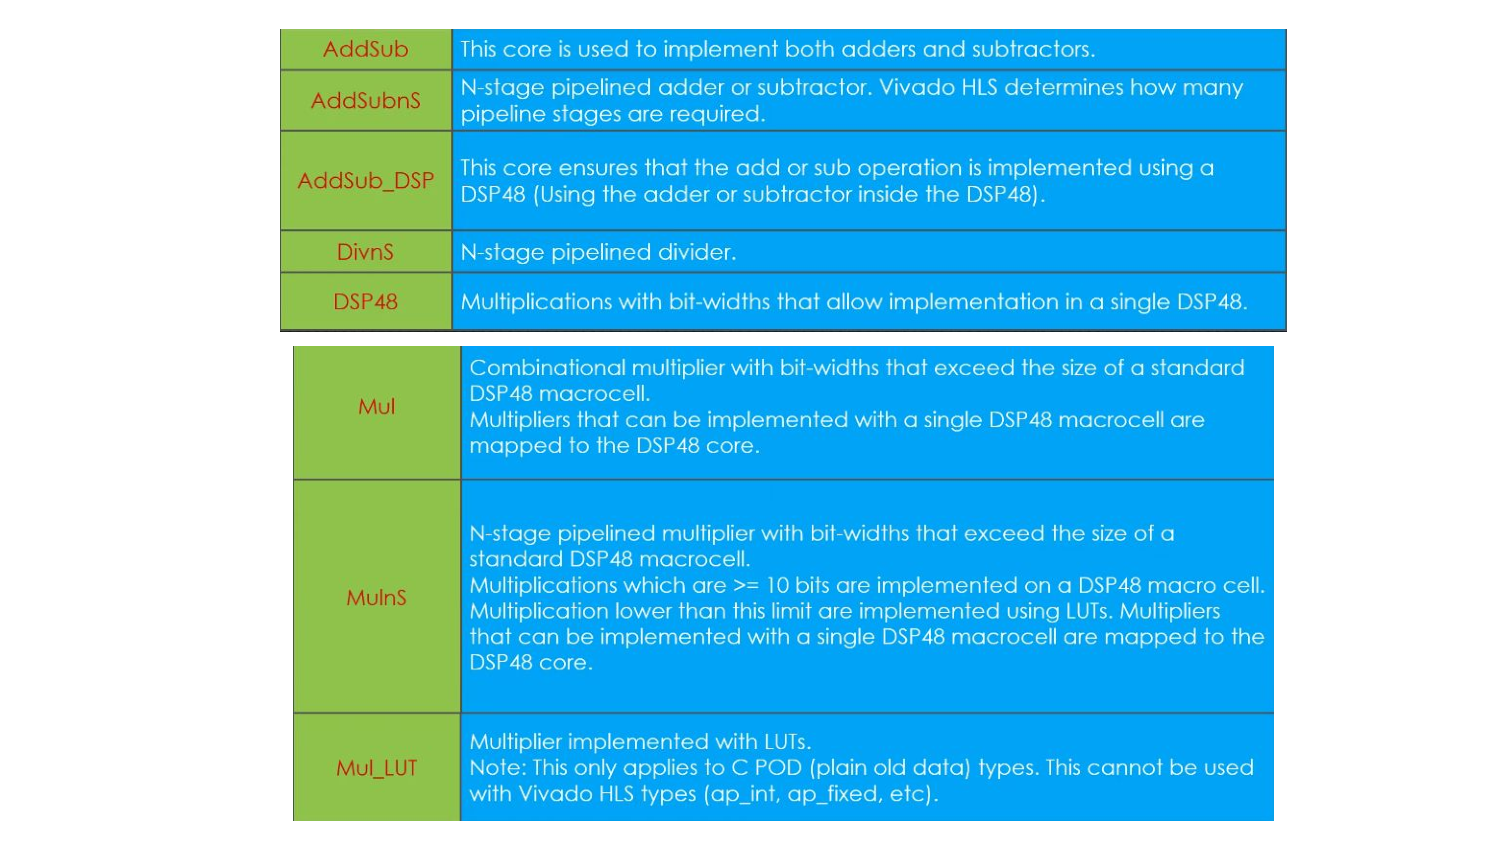
\includegraphics[scale=0.60,frame]{Figures/int_arithmetic/cores_example}
\caption{Hardware Cores Example}
\label{fig:int_arithmetic:cores_example}
\end{figure}


\subsection{Examples}

In \verb|HLS|, there are 2 pragma directive to use these core resources on operators: \verb|ALLOCATION| and \verb|RESOURCE|. 

\begin{figure}[h]
\centering
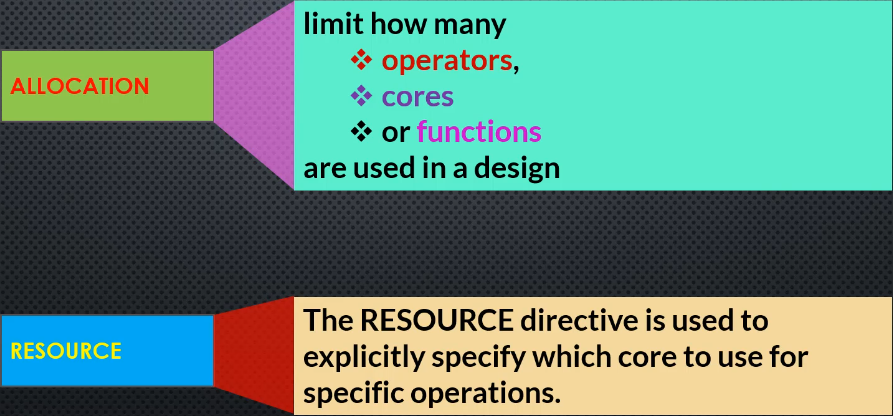
\includegraphics[scale=0.40,frame]{Figures/int_arithmetic/resrc_directive}
\caption{Resource directives}
\label{fig:int_arithmetic:resrc_directive}
\end{figure}

Let's take several examples to see how to use these directive.

\newpage
$\mathrm{1}^\mathrm{st}$ example is shown in \autoref{fig:int_arithmetic:resrc_ex1}, where \verb|f| is the output of the operator.

\begin{figure}[h]
\centering
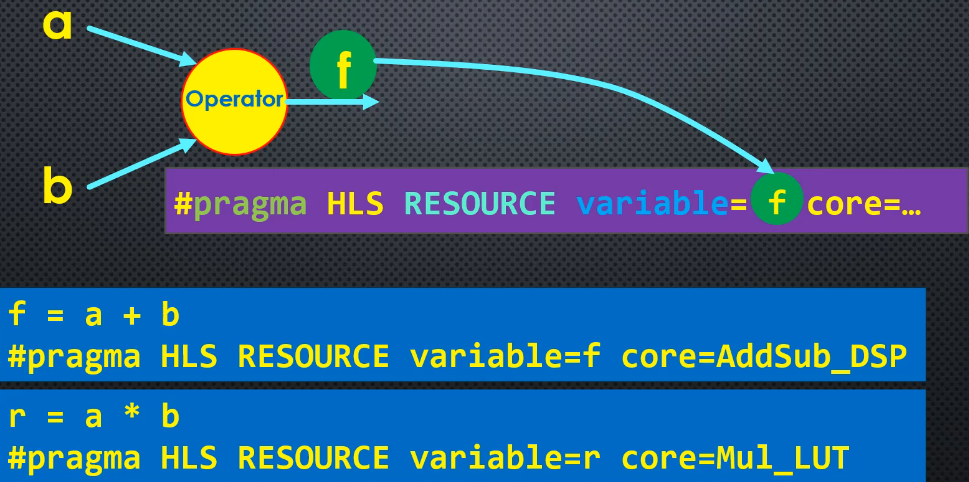
\includegraphics[scale=0.40,frame]{Figures/int_arithmetic/resrc_ex1}
\caption{Example 1 of resource usage: DSP and LUT}
\label{fig:int_arithmetic:resrc_ex1}
\end{figure}

\begin{itemize}

\item using \verb|#pragma HLS RESOURCE variable=f core=...|,  \verb|HLS| tool know which resource to use for the synthesis for the \verb|f| expression

\item 2 examples are used for the operator: \verb|+| and \verb|*|

	\begin{itemize}
	
	\item The addition is performed using DSP block through \verb|core=AddSub_DSP|

	\item The multiplication is perfomed using LUT through \verb|core=Mul_LUT|
	
	\end{itemize}

\end{itemize}

\autoref{fig:int_arithmetic:resrc_ex2} presents an expression with multiple operator. 

\begin{figure}[h]
\centering
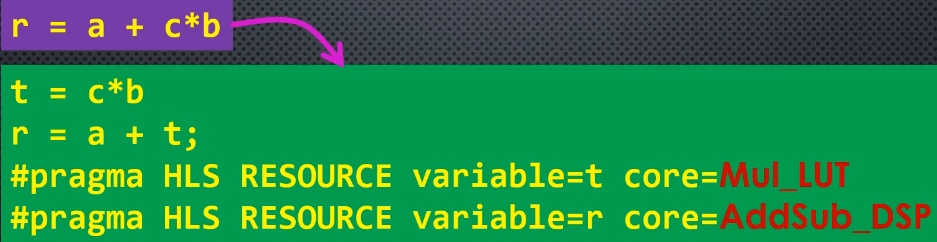
\includegraphics[scale=0.40,frame]{Figures/int_arithmetic/resrc_ex2}
\caption{Expression with multiple operators}
\label{fig:int_arithmetic:resrc_ex2}
\end{figure}

The key it to break down the expression into a set of expression of 1 opertors, then use the \verb|#pragma| on each expression.

\todo{$\mathrm{3}^\mathrm{rd}$ example} \uti{$\mathrm{3}^\mathrm{rd}$ example:}

\begin{itemize}

\item \textit{source: section 12, video 12, from time 4:22}

\item \textit{it is about implementing a complex arithmetic expression in Vitis, using LUT and DSP}

\item \textit{It uses the analysis perspective and change the clock rate}

	\begin{itemize}
	\item \textit{I didn't understand all the details yet, to redo when doing a complete revision about the $\mathrm{1}^\mathrm{st}$ part, and digital logic part also}
	\end{itemize}

\end{itemize}


\newpage
\section{Integer Division and Modulus}

Integer division and modulus need special attention when  when it comes to synthesizing them into combinational circuits.\\

As a reminder, integer division returns the quotient and modulus returns the reminder, as shown in the example of 
\autoref{fig:int_arithmetic:div_mod}.

\begin{figure}[h]
\centering
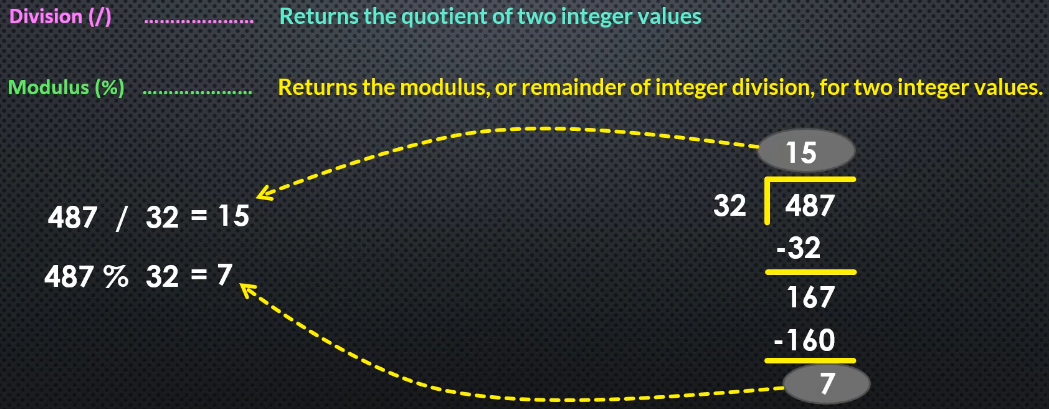
\includegraphics[scale=0.40,frame]{Figures/int_arithmetic/div_mod}
\caption{Division and Moudulus}
\label{fig:int_arithmetic:div_mod}
\end{figure}

Let's see different cases for \verb|/| and \verb|%| operations.

The pragma used: \verb|#pragma HLS RESOURCE variable=r core=Divns|.\\

\underline{Different cases:}

\begin{enumerate}

\item Division: \verb|r = a/n;|

	\begin{itemize}
	\item pipeline by default (with or no \verb|pragma| used)
	
	\item if \verb|const int n;|, then it synthesis combinational if clock period $> \, t_p$
	\end{itemize}

\item Modulus: \verb|r = a%n|

	\begin{itemize}
	\item pipeline also by default
	
	\item if \verb|const int n|, we can use the equivalent expression \verb|r = a - n*(a/n)|
	\end{itemize}

\end{enumerate}


\todo{division and moudlus demo} \uti{division and moudlus demo:}

\begin{itemize}

\item  \textit{source: section 12, video 103, t = 3:05}

\item \textit{Also various demo using Vitis, but to do later when reviweing the digital desing part, computer arithmetic,$\cdots$}

\item \textit{To see if his explanation and notes has some benifits or not, or just some theory applied}

\end{itemize}

\section{Quiz}

See the file IntegerArithmetic-Exercise-Solution in \verb|Other_Resources| directory.



\chapter{Case Study: Home Alarm System}

\section{Introduction}

We start by some projects to apply all the knowledge acquired in previous chapters concerning \verb|HLS|, combinational part. The project encountered in this chapter is about desinging an \textit{home alarm system}.\\


\subsection{System Description}
\label{sub:sys_descrip}

$\mathrm{1}^\mathrm{st}$ we start by the defintion of the system. \autoref{fig:home_alarm:proj_def} presents its description. 

\begin{figure}[h]
\centering
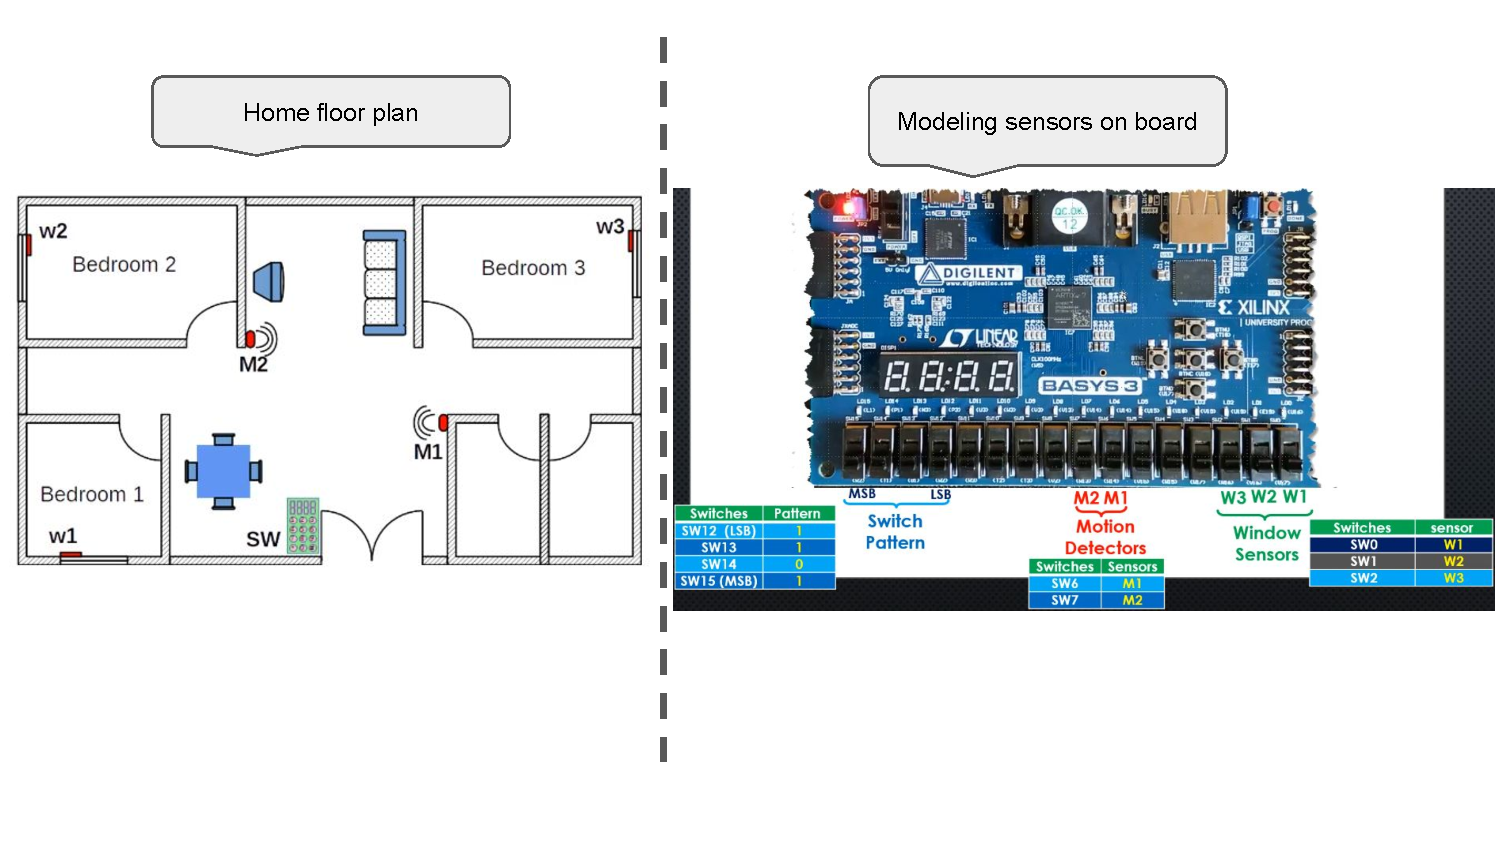
\includegraphics[scale=0.6,frame]{Figures/home_alarm/proj_def}
\caption{Home alarm system project definition}
\label{fig:home_alarm:proj_def}
\end{figure}

\begin{itemize}

\item We have 2 sets of sensors: motion and window

\item For the window: it detects the status of the window

	\begin{itemize}
	\item open window $\leftrightarrow$ logic value 1
	
	\item closed window $\leftrightarrow$ logic value 0

	\end{itemize}

\item For the motion: 1 for motion and 0 for absence of motion

\item The system (that is the set of sensors) is controlled by a control pannel

	\begin{itemize}
	\item It is activated by a pattern of 4 bit: 1101
	\end{itemize}

\item The right column of \autoref{fig:home_alarm:proj_def} contains the switch mapping to model the sensors(window and motion), and also switches for the control pannel

\end{itemize}


The different type of switches will be readed using a 16 bit variable.

\begin{figure}[h]
\centering
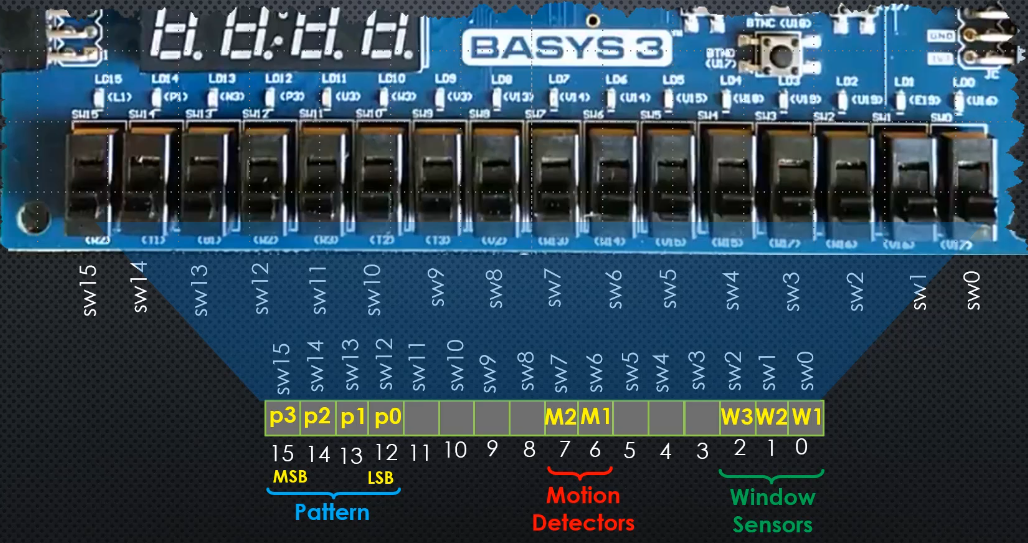
\includegraphics[scale=0.4,frame]{Figures/home_alarm/var_swtiches}
\caption{Switches Variable}
\label{fig:home_alarm:var_swtiches}
\end{figure}

\newpage
\subsection{System Status}
\label{sub:sys_stat}

To get a read for the status of the system, a 7-segement is used. The different cases for system are as follows:

\begin{itemize}

\item \autoref{tab:sys_status} contains 3 cases: system is OFF, ON and no problem is detected, and in case the sensor detects a malfunction.

\begin{table}[h]
\centering
\begin{tabular}{|c|c|}
\hline
System Status & 7-Seg Output \\
\hline
OFF & 0 \\
\hline
ON , no problem & A \\
\hline
Malfunction & E \\
\hline
\end{tabular}
\caption{System Status}
\label{tab:sys_status}
\end{table}

\item Other cases are shown in \autoref{fig:home_alarm:sys_stat_7_seg}.

\begin{figure}[h]
\centering
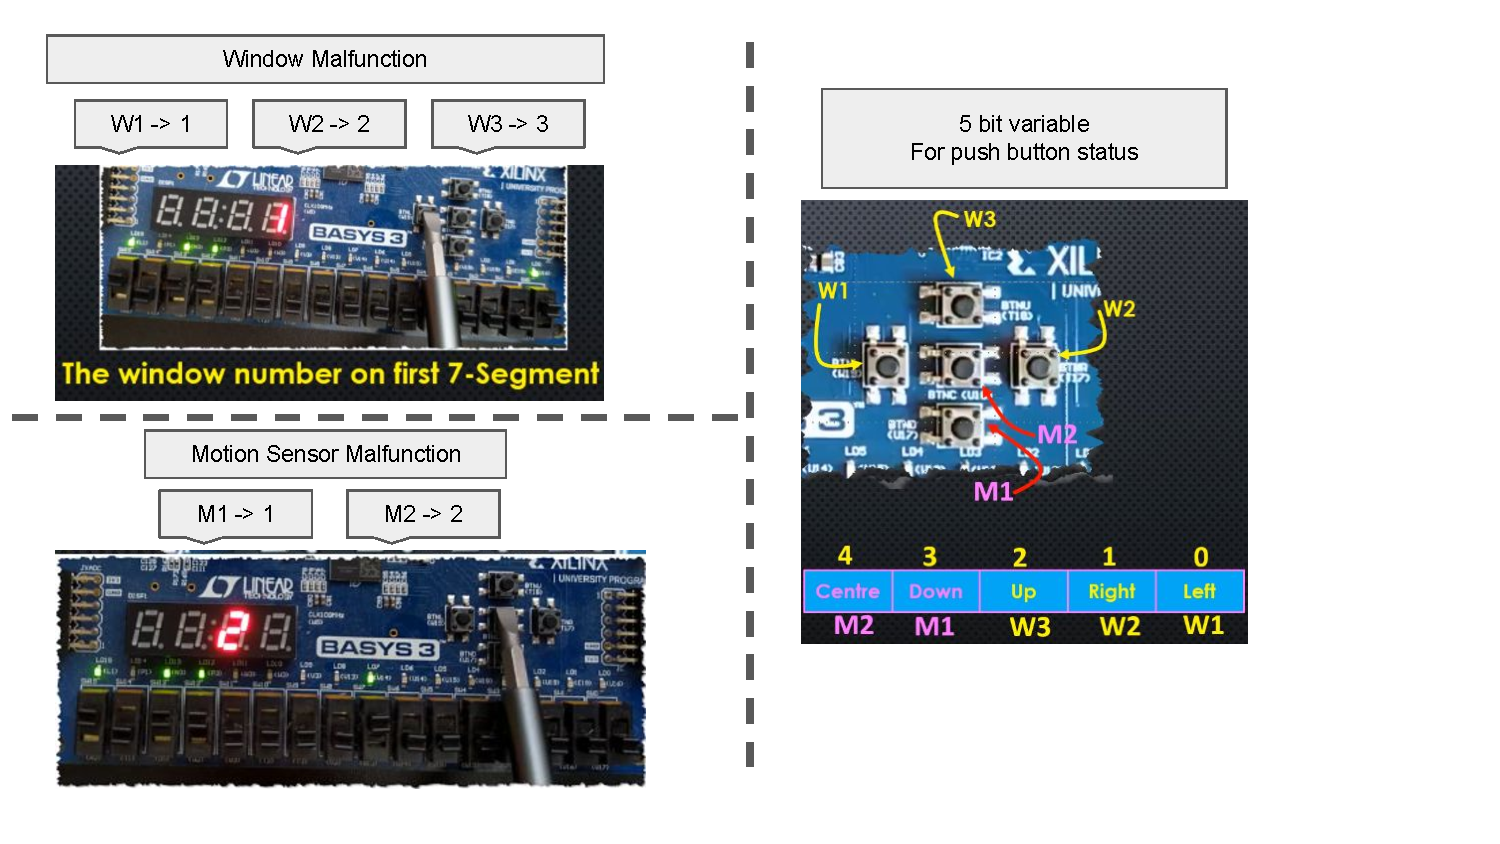
\includegraphics[scale=0.65,frame]{Figures/home_alarm/sys_stat_7_seg}
\caption{Other cases}
\label{fig:home_alarm:sys_stat_7_seg}
\end{figure}

\begin{itemize}
\item For window malfunction: $\mathrm{1}^\mathrm{st}$ digit of 7-seg is used, and motion sensor malfunction: $\mathrm{2}^\mathrm{nd}$ digit

\item Number of window or number of motion sensor is displayed  in each appropriate digit, using corresponding push button. 

\item Finally, a 5 bit variable is used to read the push button status

\end{itemize}


\end{itemize}


\newpage
\section{Code Structure}

\autoref{fig:home_alarm:code_struct} presents the code structure for the alarm system.

\begin{figure}[h]
\centering
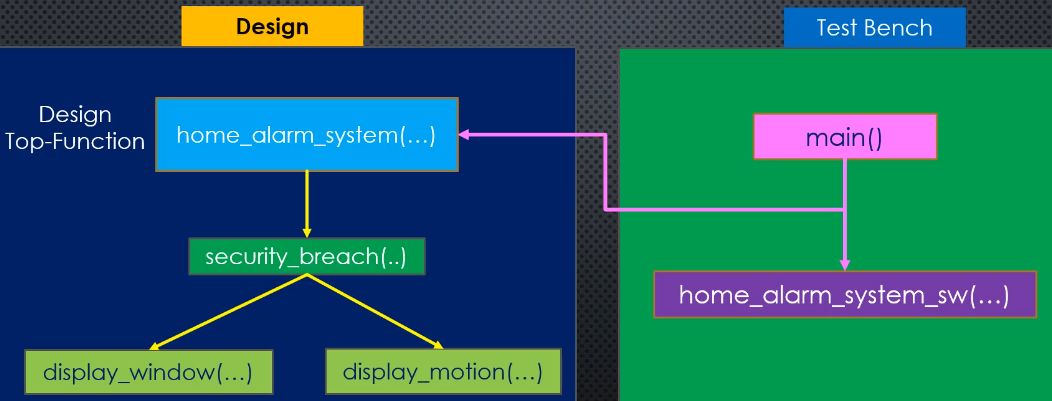
\includegraphics[scale=0.4,frame]{Figures/home_alarm/code_struct}
\caption{Code structure for alarm system}
\label{fig:home_alarm:code_struct}
\end{figure}

\begin{itemize}

\item \verb|home_alarm_system()| is the top function, where it checks all security breach, 
and send proper information for the display pannel.

\item 2 separate sub-function help to send window and motion information to the 7-segment display.

\item Finally a testbench to test the desing behaviour.	

\end{itemize}


\subsection{home-alarm-system()}

\underline{Input Output Arguments:}\\

It receives 2 group of inputs (\verb|silde_switches| and \verb|push_buttons|), and generate 3 group of outputs as shown in \autoref{fig:home_alarm:top_func}.

\begin{figure}[h]
\centering
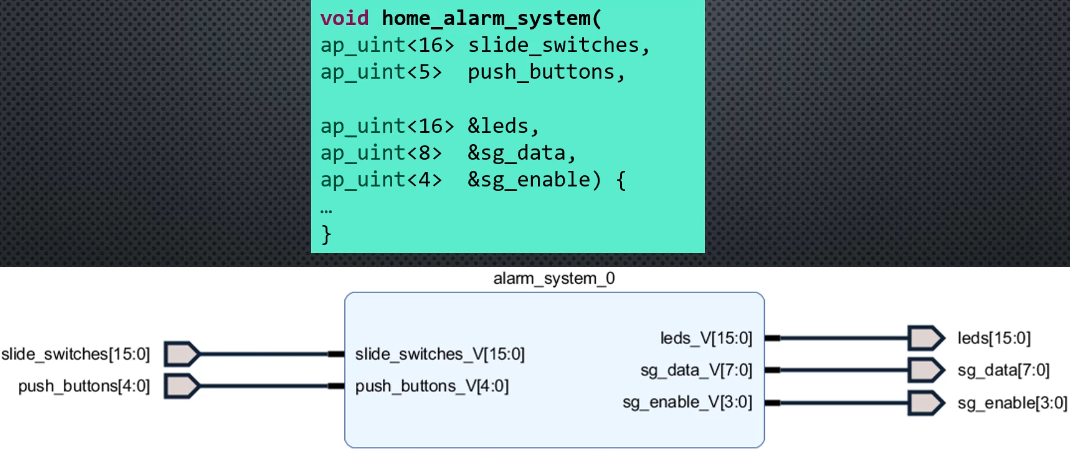
\includegraphics[scale=0.4,frame]{Figures/home_alarm/top_func}
\caption{home-alarm-system() arguments}
\label{fig:home_alarm:top_func}
\end{figure}

\newpage
As a note for the input part:

\begin{itemize}

\item \verb|silde_switches| are normal input as seen in \ref{sub:sys_descrip}.

\item \verb|push_buttons| are for fault detection, that is detect if there is some malfunction as seen in \ref{sub:sys_stat}.

\end{itemize}


The 7-segment code is defined in array as shown in \autoref{fig:home_alarm:7_seg_code_arr}, to extract the correct code and display the associated output at the 7 seg (see \autoref{sec:digit_codes}).

\begin{figure}[h]
\centering
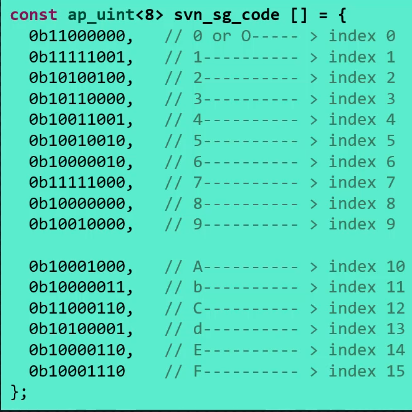
\includegraphics[scale=0.4,frame]{Figures/home_alarm/7_seg_code_arr}
\caption{7-segment code}
\label{fig:home_alarm:7_seg_code_arr}
\end{figure}

\underline{Variable Orgnisation:}\\

Recall from \ref{sub:sys_descrip} (see \autoref{fig:home_alarm:var_swtiches}) that variable switches are stored in a 16 bit variable. \autoref{fig:home_alarm:top_func_steps} contains some of the steps done in the top function:

\begin{figure}[h]
\centering
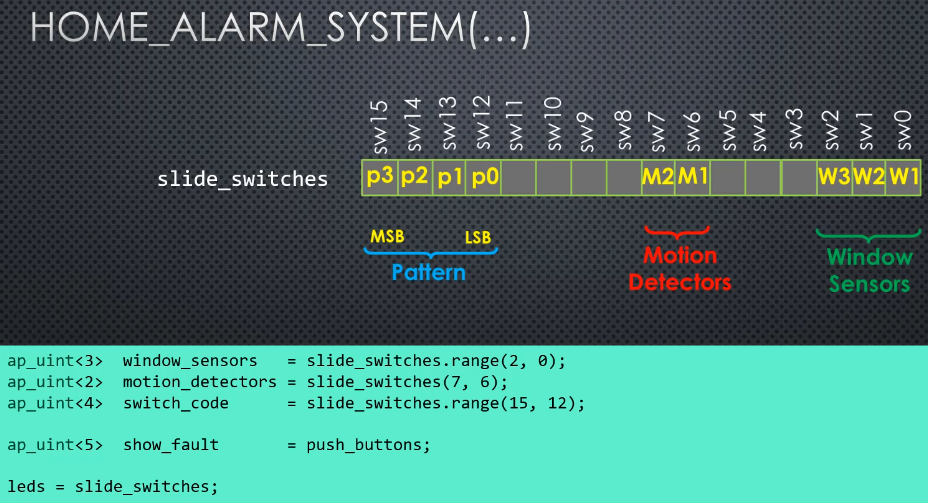
\includegraphics[scale=0.4,frame]{Figures/home_alarm/top_func_steps}
\caption{Top function steps}
\label{fig:home_alarm:top_func_steps}
\end{figure}

\begin{itemize}

\item split the 16 bit \verb|slide_switches| variable into a set of variables

\item stores the \verb|push_buttons| variable into a more descriptive name

\item connect the \verb|slide_switches| directly to the LED

\end{itemize}

\newpage

\underline{System Checking:}\\

\autoref{fig:home_alarm:top_func_checking} shows the checking done.

\begin{figure}[h]
\centering
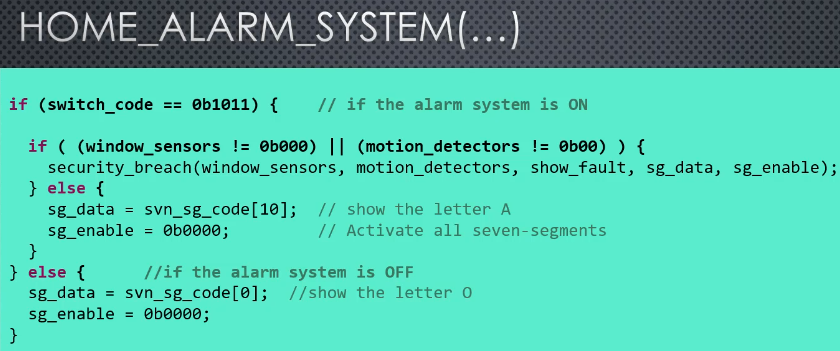
\includegraphics[scale=0.4,frame]{Figures/home_alarm/top_func_checking}
\caption{Top function checking}
\label{fig:home_alarm:top_func_checking}
\end{figure}

\begin{itemize}

\item We check $\mathrm{1}^\mathrm{st}$ the status of the system via the code of the control pannel 

$\leftrightarrow$ \verb|switch_code == 0b1011|

\item If the system is ON,we check for the window and motion sensors

\item if there is not problem, lettre \verb|A| is displayed at the 7 seg (as seen in \autoref{tab:sys_status})

\item If there is a problem, we call \verb|security_breach()| 

\end{itemize}

\subsection{security-breach()}

Now we start by the $\mathrm{2}^\mathrm{nd}$ function \verb|security_breach()|.

\begin{figure}[h]
\centering
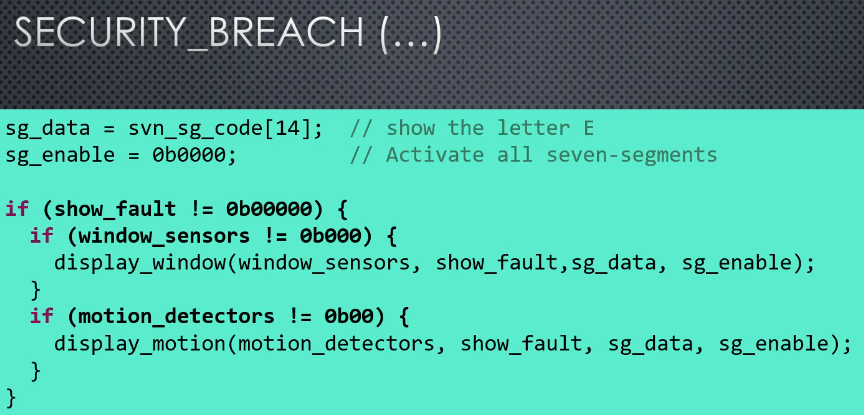
\includegraphics[scale=0.4,frame]{Figures/home_alarm/security_breach_fun}
\caption{security-breach() code}
\label{fig:home_alarm:security_breach_fun}
\end{figure}

\begin{itemize}

\item Initially, it sends the lettre \verb|E| to all 7-seg display.

\item If any of the push button is pressed, $\leftrightarrow$ \verb|show_fault != 0b00000|

it checks if we have an error on the window or motion sensor side.

\end{itemize}


\subsection{diplay-window() and display-motion()}

Functions \verb|diplay_window()| and \verb|display_motion()| are shown in \autoref{fig:home_alarm:disp_win_mot_fun}.


\begin{figure}[h]
\centering
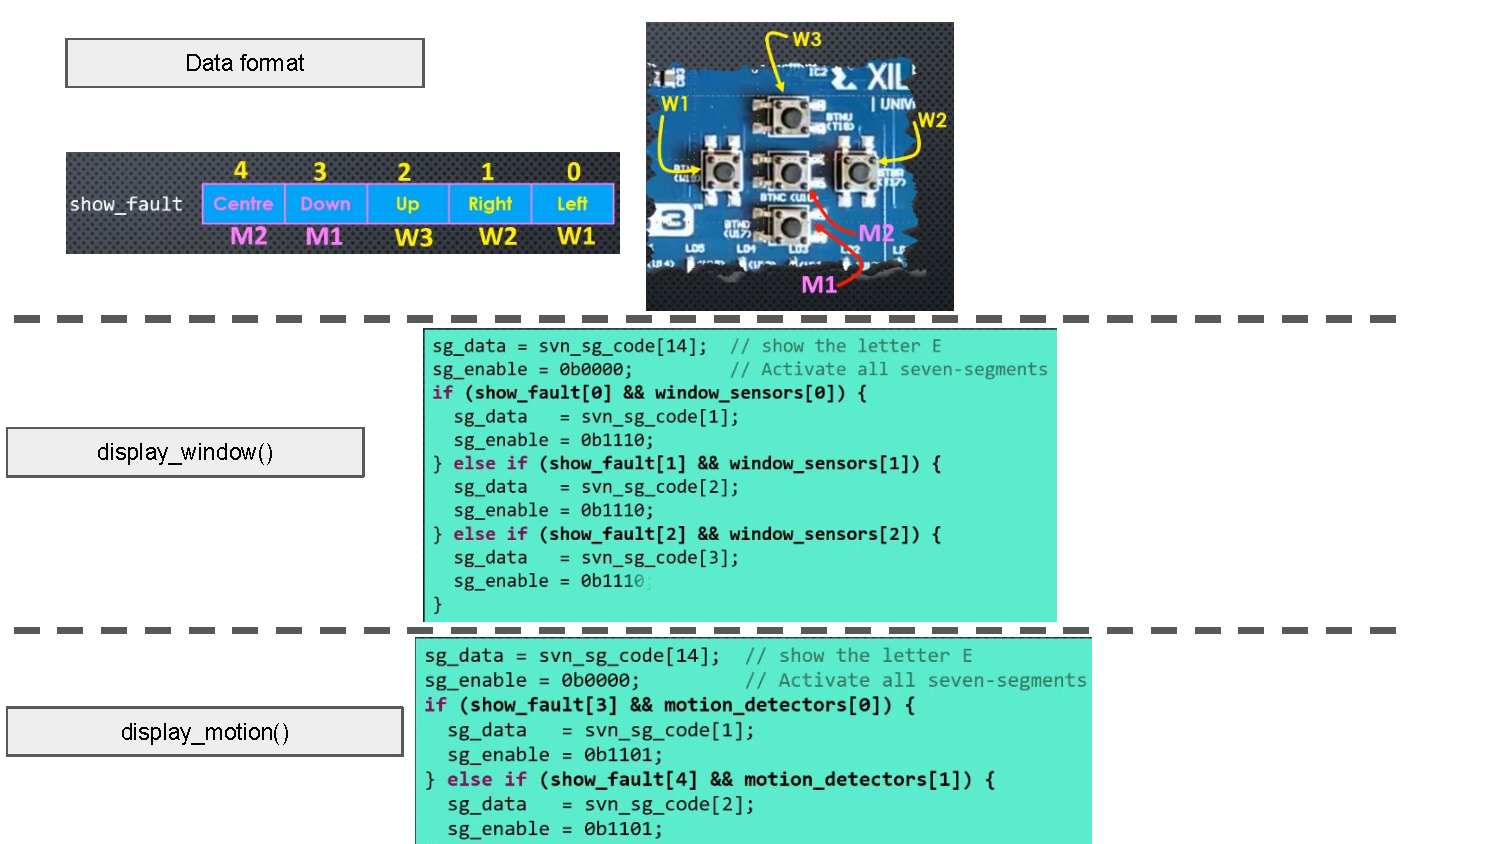
\includegraphics[scale=0.65,frame]{Figures/home_alarm/disp_win_mot_fun}
\caption{diplay-window() and display-motion() code}
\label{fig:home_alarm:disp_win_mot_fun}
\end{figure}

\begin{itemize}

\item In both function, lettre \verb|E| is again displayed into the 7 seg, so we can ensure that the data path is initialized correctly in all part of the \verb|HLS| code

	\begin{itemize}
	\item Otherwise, if we only initialize it using \verb|security_breach()|, the \verb|HLS| tool may use previous value and synthesis some flip flops elements, and the resulting circuit is no combinational anymore.
	\end{itemize}

	

\end{itemize}







\part{Sequential Circuit}
\label{part:sequential}



\end{document}
